%%%%%%%%%%%%%%%%%%%%%%%%%%%%%%%%%%%%%%%%%%%%%%%%%%%%%%%%%%%%%%%%%%%%%%%%%%%%%
%%%
%%% File: thesis.tex, version 1.7, March 2021
%%%
%%% =============================================
%%% This file contains a template that can be used with the package
%%% cs.sty and LaTeX2e to produce a thesis that meets the requirements
%%% of the Computer Science Department from the Technical University of Cluj-Napoca
%%%%%%%%%%%%%%%%%%%%%%%%%%%%%%%%%%%%%%%%%%%%%%%%%%%%%%%%%%%%%%%%%%%%%%%%%%%%%

\documentclass[12pt,a4paper,twoside]{report}

\usepackage{cs}
\usepackage[T1]{fontenc}
\usepackage[utf8]{inputenc}
\usepackage[romanian]{babel}
\usepackage{times}
\usepackage{graphicx}
\usepackage{latexsym}
\usepackage{amsmath,amsbsy}
\usepackage{amssymb}
\usepackage[matrix,arrow]{xy}
\usepackage{ae,aecompl}
\usepackage{amstext}
\usepackage{graphics}
\usepackage{ae,aecompl}
\usepackage{algorithm}
\usepackage{color}
\usepackage{titlesec}
\usepackage{fancyhdr}
\usepackage{hyperref}
%% decomentati linia urmatoare pentru e nu mai evidenția hiper legăturile pentru imprimare pe hârtie
\hypersetup{hidelinks}
\usepackage{geometry}
\usepackage{lipsum}
\usepackage{enumitem}

%%%%%%%%%%%%%%%%%%%%%%%%%%%%%%%%%%%%%%%%%%%%%%%%%%%%%%%%%%%%%
\setlist{noitemsep,nolistsep}


\diplomathesis
\centerchapter
\singlespace
\newenvironment{definition}[1][Definiție.]{\begin{trivlist}
\item[\hskip \labelsep {\bfseries #1}]}{\end{trivlist}}

%%% setari pagină
 \geometry{
	a4paper,
	total={159.2mm,246.2mm},
	left=25.4mm,
	top=25.4mm,
}


\begin{document}
%\frontmatter
%%%%%%%%%%% Stil pentru paginile de capăt
\pagestyle{fancy}
\setlength{\voffset}{-10pt}
\setlength\headheight{70.0pt}
%\addtolength{\textheight}{-80.0pt}
\renewcommand{\headrulewidth}{0pt}
\chead{%
	
\includegraphics[width=\textwidth]{figs/AntetUTCNRom.pdf}
}
\cfoot{}
\lfoot{}
\rfoot{}
%%%%%%%%%%%%%%%%%%%%%%%%%%%%%% Schimbați corespunzător ultimul element
\renewcommand{\thesisauthor}{Mihai-Octavian COPOSESCU}    %% Prenumele și numele dvs.
\renewcommand{\thesismonth}{Iulie}     %% Luna sesiunii de licență
\renewcommand{\thesisyear}{2024}      %% Anul sesiunii de licență
\renewcommand{\thesistitle}{Sistem de monitorizare a calitatii aerului} % Titlul luucrării de licență
\renewcommand{\thesissupervisor}{Prof. Dr. Ing. Zoltan Francisc BARUCH} %% Conducătorul științific
%%%%%%%%%%%%%%%%%%%%%%%%%%%%%%%%%%%%%
\newcommand{\makeThesisTitle}{\textbf{\thesistitletypesize \thesistitle}}
\newcommand{\makeThesisType}{\thesistypetypesize \thesistype}
\newcommand{\department}{\sffamily\bfseries\small FACULTATEA DE AUTOMATICĂ ȘI CALCULATOARE\\
	DEPARTAMENTUL CALCULATOARE} 
\renewcommand{\thesistype}{LUCRARE DE LICENȚĂ}
\newcommand{\uline}[1]{\rule[0pt]{#1}{0.4pt}}
% Headings pentru folie de capăt
%%%%% Pagina cu titlul tezei nu trebuie să schimbati nimic %%%%%%%%%%%%%%%%%%%%%%%%
\begin{center}
	{\department}
	
	\vspace{4cm}
	\makeThesisTitle
	~\\~\\
	
	\makeThesisType
	
	~\\\vspace{6.5cm}
	
	\begin{tabular}{p{.3\linewidth}p{.5\linewidth}}
		{\hfill Absolvent:} & {\bf \thesisauthor} \\
		&\\
		{\parbox[t]{\linewidth}{\qquad\qquad\qquad Coordonator\\\hspace*{3.2cm}științific:}}& {\bf \thesissupervisor}\\
	\end{tabular}
	
	\vspace{3cm}
	{\bf \thesisyear}
\end{center}
%%%%%%%%%%%%%%%%%%%%%%%%%%%%%%%%%%%%%%%%%%%%%%%%%%%%%
\newpage
%%%%%%% Pagina cu tema %%%%%%%%%%%%%%%%%%%%%%%%%%%%%%%
\begin{center}
	{\department}
\end{center}
\vspace{0.5cm}

%\begin{small}
\begin{tabular}{p{7cm}p{8cm}}
	%\hspace{-1cm}& VIZAT,\\
	\hspace{-1cm}DECAN, & DIRECTOR DEPARTAMENT,\\
	\hspace{-1cm}{\bf Prof. dr. ing. Mihaela DÎNȘOREANU} & {\bf Prof. dr. ing. Rodica POTOLEA}\\  
\end{tabular}

\vspace{2cm}

\begin{center}
	Absolvent: {\bf \thesisauthor}
	
	\vspace{1cm}
	
	{\bf \thesistitle}
\end{center}

\vspace{5mm}
%%%%%%%%%%%%%%%%%%%%%%% Aici modificați
\begin{enumerate}
	\item {\bf Enunțul temei:} {\it Proiectarea unui sistem de monitorizare a calitatii aerului unui mediu care include achizitia de date, gestiunea datelor 
	si prezentarea acestora utilizatorului final}
	\item {\bf Conținutul lucrării:} {\it Introducere, Obiectivele proiectului, Studiu bibliografic, Analiza si fundamentare teoretica, Proiectare de detaliu si 
	implementare, Testare si validare, Manual de instalare si utilizare, Concluzii, Bibliografie.}
	\item {\bf Locul documentării:} Universitatea Tehnică din Cluj-Napoca, Departamentul Calculatoare
	\item {\bf Consultanți:}
	\item {\bf Data emiterii temei:} 12 Martie 2024 %%%%%%%%%%%%% Modificați corespunzător
	\item {\bf Data predării:} 2 Septembrie 2024 %%%%%%%%%%%%%%% Modificați corespunzător
\end{enumerate}
\vspace{1.2cm}

\hspace{6cm} Absolvent: \uline{6cm} 

\vspace{0.5cm}
\hspace{6cm} Coordonator științific: \uline{5cm} 
\newpage
%%%%%%%%% Pagina cu declarația
\begin{center}
	{\department}
\end{center}
\vspace{0.5cm}

\begin{center}
	{\bf Declarație pe propria răspundere privind\\ 
		autenticitatea lucrării de licență}
\end{center}
\vspace{1cm}

\begin{minipage}{\linewidth}
	\indent Subsemnatul, Coposescu Mihai-Octavian %% locul pentru nume prenume
	legitimat cu CI %% locul pentru tipul documentului de identitate
	seria HD % seria documentului de identitate 
	nr. 944105 % numărul documentului de identitate 
	CNP 1970115203401, % CNP
	autorul lucrării "Sistem de monitorizare a calitatii aerului"
	elaborată în vederea susținerii examenului de finalizare a studiilor de licență la Facultatea de Automatică și Calculatoare, Specializarea Calculatoare % numele specializării
	din cadrul Universității Tehnice din Cluj-Napoca, sesiunea Septembrie % numele sesiunii de licență (luna)
	a anului universitar 2023-2024, % anul de început al anului universitar
	declar pe propria răspundere că această lucrare este rezultatul propriei activități intelectuale, pe baza cercetărilor mele și pe baza informațiilor obținute din surse care au fost citate, în textul lucrării și în bibliografie.\\
	\hspace*{8mm} Declar că această lucrare nu conține porțiuni plagiate, iar sursele bibliografice au fost folosite cu respectarea legislației române și a convențiilor internaționale privind drepturile de autor.\\
	\hspace*{8mm} Declar, de asemenea, că această lucrare nu a mai fost prezentată în fața unei alte comisii de examen de licență.\\
	\hspace*{8mm} În cazul constatării ulterioare a unor declarații false, voi suporta sancțiunile administrative, respectiv, \emph{anularea examenului de licență}.
\end{minipage}
\vspace{1.5cm}

Data \hspace{8cm} Nume, Prenume

\vspace{0.5cm}

02.09.2024 \hspace{5cm} Coposescu Mihai-Octavian

\vspace{1cm}
\hspace{9.4cm}Semnătura
\newpage
 % Primele 3 pagini
%%%%%%%%%%%%%%%%% Pagina cu instructiuni de eliminat
\thispagestyle{empty}
\thispagestyle{empty}
\begin{center}\large
	Instrucțiuni generale.
\end{center}
~\\

{\color{red}\large{\bf De citit înainte} (această pagină se va elimina din versiunea finală)}:\\
\begin{enumerate}
 \item Cele trei pagini anterioare (foaie de capăt, foaie sumar, declarație) se vor lista pe foi separate (nu față-verso), fiind incluse în lucrarea listată.
 Foaia de sumar (a doua) necesită semnătura absolventului, respectiv a coordonatorului.
 Pe declarație se trece data când se predă lucrarea la secretarii de comisie.
 \item Pe foaia de capăt, se va trece corect titulatura cadrului didactic îndrumător, în engleză (consultați pagina de unde ați descărcat acest document pentru lista cadrelor didactice cu titulaturile lor).
 \item Fiecare capitol începe pe pagină nouă.
 \item Marginile paginilor nu se modifică.
 \item Respectați restul instrucțiunilor din fiecare capitol.
 \item Am inclus pachetul \verb+hyperref+ pentru a genera legături de navigare atât în document cât și la link-uri de web. Pentru listarea pe hârtie a fișierului pdf decomentați linia care conține \verb+%\hypersetup{hidelinks}+
 aflată în partea de început a fișierului principal \verb+thesis_rom.tex+.
\end{enumerate}

\newpage
%%%%%%%%%%%%%%%%%% sf. pagina cu instructini
\pagestyle{fancy}
\setlength\headheight{16.0pt}
\renewcommand{\chaptermark}[1]{\markboth{\chaptername~\thechapter.~#1}{}}
\renewcommand{\sectionmark}[1]{\markright{\thesection\ #1}}
\renewcommand{\headrulewidth}{0.4pt}
\lhead{}
\chead{%
	\leftmark\rightmark
}
\chead{}
\cfoot{\thepage}
\lfoot{}
\rfoot{}

%%%%%%%%%%%% Cuprinsul %%%%%%%%%%%%%%%%%%%%%%%%%%%%%%%%%%%%%%%%
\pagenumbering{roman}
\setcounter{page}{1}

\newpage

\tableofcontents

\newpage

%\listoftables
%\listoffigures

%%%%%%%%%%%%%%%%%% de aici începe numerotarea paginilor
\pagenumbering{arabic}
\setcounter{page}{1}


\titleformat{\chapter}[hang]
{\normalfont\Large\bfseries}{\chaptertitlename\ \thechapter.}{1em}{}
\titleformat{\section}[hang]
{\normalfont\large\bfseries}{\thesection.}{1em}{}
\titleformat{\subsection}[hang]
{\normalfont}{\thesubsection.}{1em}{}
\titlespacing*{\section}{0pt}{12pt}{6pt}
\titlespacing*{\subsection}{0pt}{12pt}{6pt}
\titlespacing*{\chapter}{0pt}{30pt}{18pt}

\chapter{Introducere}\label{ch:intro}
\pagestyle{fancy}

{\color{blue}\noindent Capitolul va ocupa 2-3 pagini.\\}
\noindent Ce se scrie aici:

\begin{itemize}
	\item Contextul temei
	\item Conturarea domeniului exact al temei
\end{itemize}

 % \chapter{Introducere}

\chapter{Obiectivele proiectului}\label{ch:obiective}
\pagestyle{fancy}

{\noindent\color{blue}Se va întinde pe 2-3 pagini.\\}

În acest capitol se prezintă tema propriu-zisă (sub forma unei teme de proiectare sau cercetare, formulată exact, cu obiective clare și eventuale figuri explicative).

 % \chapter{Obiectivele Proiectului}

\chapter{Studiu bibliografic}\label{ch:studiubib}

\pagestyle{fancy}

In cadrul acestui capitol vor fi prezentate sisteme de monitorizare a calitatii aerului asemanatoare cu cel prezentat in lucrarea de fata.

Majoritatea sistemelor de monitorizare a calitatii aerului de pe piata in momentul redactarii acestei lucrari nu ofera suport pentru acesarea datelor de 
la distanta sau accesarea datelor istorice. Acestea sunt concepute cu un ecran mare pe care sunt afisate ultimele valori citite ale metricilor de calitate a 
aerului sau grafice pe intervale mici de timp. Aceste metrici sunt acompaniate de culori care codifica anumite intervale de valori de la calitatea aerului 
foarte buna pana la calitatea aerului foarte slaba si, uneori, de un sunet de alarma atunci cand calitatea aerului este considerata slaba.

In urmatoarele sectiuni sunt prezentate sisteme de monitorizare a calitatii aerului care au urmatoarele caracteristici: senzorul are capabilitatea de conectare 
la o retea Wi-Fi, datele sunt gestionate in cloud si aplicatie pe telefonul mobil sau web pentru vizualizarea metricilor colectate de sonzori.

\section{Solutia Airthings}\label{sec:airthingsWavePlus}
\subsection{Descriere}\label{subsec:airthings_descriere}
Solutia oferita de compania Airthings se concentreaza pe calitatea aerului in spatii inchise. Aceasta include senzori de calitate a aerului, un gateway si conexiune 
de la distanta prin intermediul unei aplicatii mobile si a unei pagini web. Informatiile continute in acest capitol au fost extrase de pe site-ul oficial de 
prezentare al companiei Airthings si din manualele de instalare si de depanare puse la dispozitie de acesta \cite{airthings}.

Aceasta solutie poate fi impartita in 2 categorii, conexiune bluetooth si conexiune prin gateway. Conexiunea bluetooth are ca tinta spatiile inchise mici, 
cum ar fi locuintele care necesita un numar mic de senzori, intre 1 si 3 senzori. Conexiunea prin gateway are ca tinta spatiile inchise mari, cum ar fi cladirile de 
birouri unde este necesar un numar mai mare de senzori, intre 3 si 10 senzori.

Figura \ref{fig:sb_airthingsNetwork} prezinta solutia oferita de Airthings. In paragrafele urmatoare sunt descrise modulele prezentate in aceasta figura.
\begin{figure}[H]
    \centering
    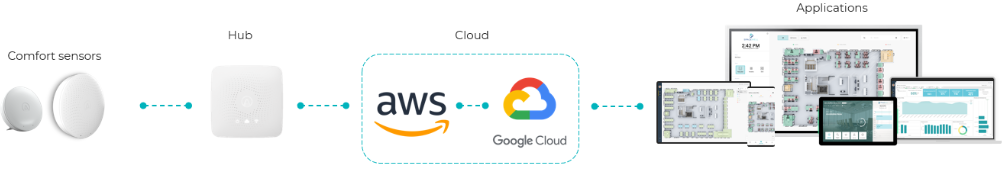
\includegraphics[scale=0.6]{figs/sb_airthingsNetwork.png}
    \caption{Reteaua Airthings}
    \label{fig:sb_airthingsNetwork}
\end{figure}

Modulul senzor are rolul de a achizitiona metrici de calitate a aerului si de a le transmite catre modulul Hub. Acesta functioneaza pe baterii si are o durata de 
viata de pana la 15 luni. Protocolul de comunicatie utilizat in reteaua interna compusa din senzori si gateway se numeste SmartLink si este un protocol proprietar 
dezvoltat de compania Airthings. Banda de frecventa in care senzorii comunica cu gatewayul este 868 MHz pentru Europa si 915 MHz pentru Statele Unite. Utilizarea 
acestei benzi de frecventa ofera o raza de acoperire a comunicatiei mai mare decat banda 2.4 GHz, mai ales in spatii inchise care contin multe obstacole.

Modulul Hub reprezinta gatewayul sistemului. Acesta are rolul de interfata intre senzori si internet, centralizand datele receptionate de la senzori si tranferandule 
mai departe in cloud. Conexiunea la internet se poate realiza prin cablu ethernet sau printr-o cartela SIM preinstalata de producator. Numarul maxim de senzori care 
pot fi conectati la modulul Hub este 10.

Modulul Cloud are rolul de a salva datele intr-o baza de date si de a oferi date istorice si date in timp real modulului Aplications.

Modulul Aplications ofera o interfata web sau pe telefonul mobil care afiseaza utilizatorului datele colectate de la senzori intr-un mod intuitiv.

Senzorii au capacitatea de a comunica si prin standarul Bluetooth direct cu aplicatia de pe telefonul mobil. In cazul acesta datele colectate de senzori sunt 
mentinute in memoria acestuia si transferate catre aplicatie atunci cand exista conexiune Bluetooth. Aplicatia are capacitatea de a monitoriza mai multi senzori 
in acelasi timp daca exista conexiune.

Airthings ofera mai multe tipuri de senzori care se deosebesc prin metricile de calitate a aerului colectate. Cel mai complex dintre acestea este Airthings Wave 
Plus care colecteaza urmatoarele metrici:
\begin{itemize}
	\item Gazul radioactiv Radon.
	\item Dioxid de Carbon (CO2).
	\item Concentratia Compusilor Organici Volatili Totala (TVOC)
	\item Umiditate.
	\item Temperatura.
	\item Presiunea Aerului.
\end{itemize}

\subsection{Avantaje}\label{subsec:airthings_avantaje}
\begin{itemize}
	\item Colectarea metricii radon.
	\item Functionarea pe baterii pana la 15 luni.
\end{itemize}

\subsection{Dezavantaje}\label{subsec:airthings_dezavantaje}
\begin{itemize}
	\item Numarul maxim de 10 senzori suportati de gateway este mic in cazul cladiririlor de birouri.
	\item Fara achizitionarea unui gateway, datele istorice care pot fi accesate sunt pe o perioada foarte scurta, limitata de memoria interna a senzorilor.
\end{itemize}

\section{Solutia Awair}\label{sec:awair}
\subsection{Descriere}\label{subsec:awair_descriere}
Solutia oferita de compania Awair este asemanatoare cu cea oferita de compania Airthings. Aceasta se concentreaza pe spatii inchise si include senzori de calitate 
a aerului, un gateway in anumite configuratii de retea, un server in cloud si aplicatie web sau pe telefon pentru gestiunea datelor. Ofera doua tipuri de senzori, 
unul pentru locuinte si unul pentru cladiri mari, cum ar fi scoli sau cladiri de birouri. Informatiile continute in acest capitol au fost extrase de pe site-ul oficial de 
prezentare al companiei Awair si din manualele de instalare si de depanare puse la dispozitie de acesta \cite{awair}.

Solutia oferita de Awair pentru locuinte este senzorul Awair Element. Acesta este un senzor de sine statator capabil de crearea unei conexiuni prin protocolul 
Bluetooth sau prin protocolul Wi-Fi. Acesta este destinat pentru utilizarea impreuna cu un router uzual. Conexiunea Bluetooth este utilizata la instalarea senzorului 
unde, prin aplicatia pentru telefon Awair Home se realizeaza conexiunea Bluetooth si se transmit catre senzor informatii despre routerul la care acesta urmeaza sa 
se conecteze. La finalul procesului de instalare senzorul opreste conexiunea Bluetooth cu telefonul si se conecteaza la routerul despre care a primit informatii 
prin protocolul Wi-Fi. Din acest moment senzorul transmite periodic date catre serverul cloud. Aceasta solutie este foarte asemanatoare cu lucrarea de fata, cu 
exceptia capabilitatii de conectare prin Bluetooth pentru procesul de instalare.

Pentru spatii inchise mari Awair ofera o alta solutie care contine unul sau mai multi senzori numiti Awair Omni si un gateway numit Await Net. Senzorul Awair 
Omni este capabil de realizarea a trei tipuri de conexiuni:
\begin{itemize}
	\item Bluetooth - pentru procesul de instalare al senzorului.
	\item Wi-Fi - pentru utilizarea senzorului Awair Omni in acelasi mod in care este utilizat Awair Element.
	\item LoRa - pentru comunicatia dintre senzori si gateway.
\end{itemize}
Gatewayul Await Net poate fi conectat la internet utilizand un cablu ethernet sau o cartela SIM. Acesta comunica cu senzorii utilizand un protocol de comunicatie 
proprietar la baza caruia, in nivelul fizic al stivei de comunicatie, se afla tehnica LoRa. Banda de frecventa in care acesta comunica este 868 MHz pentru Europa 
si 915 MHz pentru Statele Unite. Senzorii au capabilitatea de repetor, ceea ce ofera posibilitatea crearii unei retele mesh. Distanta la care senzorii comunica 
in linie dreapta fara obstacole este de aproape un kilometru, iar prin capacitatea crearii unei retele mesh aceasta poate fi extinsa. In reteaua mesh fiecare 
senzor are un nod principal prin care comunica si o lista de cai secundare utilizate in cazul deteriorarii comunicatiei sau a caderii conexiunii cu nodul principal.

Senzorii sunt alimentati de la o sursa de 5V printr-un cablu USB type-C si achizitioneaza urmatoarele metrici de calitate a aerului:
\begin{itemize}
	\item Particulele in suspensie PM2.5 si PM10.
	\item Dioxid de Carbon (CO2).
	\item Concentratia Compusilor Organici Volatili Totala (TVOC).
	\item Umiditate.
	\item Temperatura.
	\item Lumina ambientala.
	\item Zgomotul ambiental.
\end{itemize}

Un al treilea tip de senzor oferit de awair se numeste Glow C, iar scopul acestuia este de integrare cu sistemele existente in locuinte sau in cladirile de birouri 
care nu suporta o conexiune Wi-Fi. Acest senzor este o extensie de stecher cu o priza care are capabilitatea de conectare Wi-Fi. In priza oferita de senzor poate fi 
conectat un sistem care nu suporta conexiune Wi-Fi, iar acesta va fi controlat de catre senzor prin pornirea si oprirea alimentarii bazat pe datele de calitate a 
aerului colectate de acesta. Exemple de astfel de sisteme sunt: un ventilator, un calorifer electric etc. De asemenea, acesta ofera o sursa de lumina LED care isi 
schima culoarea in functie de calitatea aerului detectat: Verde insemnand o calitatea a aerului buna, portocaliu insemnand o calitate a aerului acceptabila si rosu 
insemnand o calitate a aerului slaba.

Majoritatea senzorilor oferiti de Awair pot fi integrati cu asistentii virtuali Alexa, Google Home sau IFTTT.

\subsection{Avantaje}\label{subsec:awair_avantaje}
\begin{itemize}
	\item Capacitatea de acoperire a unei arii foarte mari datorata utilizarii protocolului LoRa si al capacitatii de creeare a unei retele mesh.
	\item Integrarea cu sisteme care nu suporta conexiune fara fir.
\end{itemize}

\section{Solutia Air Quality Egg}\label{sec:airqualityegg}
\subsection{Descriere}\label{subsec:airqualityegg_descriere}
Solutia oferita de compania Air Quality Egg este o platforma de dezvoltare destinata persoanelor pasionate de domeniul calitatii aerului. Datele colectate de catre 
senzorii din intreaga lume sunt disponibile intr-o platforma web oricarei persoane interesate in analiza acestora. Informatiile continute in acest capitol au fost 
extrase de pe site-ul oficial de prezentare al companiei Air Quality Egg si din manualele de instalare si de depanare puse la dispozitie de acesta \cite{airqualityegg}.

Senzorul, numit The Egg, este format dintr-o platforma hardware ale carei detalii sunt publice si utilizeaza un software care, la randul lui, este public. Aceste 
informatii sunt publice in scopul dezvoltarii rapide, orice persoana poate oferi solutii la probleme curente sau poate aduce imbunatatiri sistemului. Toti senzorii 
Egg colecteaza urmatoarele metrici de calitate a aerului: temperatura, umiditate si presiune. Pe langa acestea, la comandarea unui senzor nou este oferita o 
lista cu metrici suplimentare de calitate a aerului din care pot fi selectate cele dorite de cumparator. Acest lucru inseamna ca Air Quality Egg incepe productia 
unui senzor doar dupa plasarea unei comenzi, ceea ce face ca durata de receptie a senzorului sa fie mai lunga, aproximativ 4 saptamani.

Figura \ref{fig:sb_airqualityeggmap} prezinta senzorii Egg din intreaga lume. Afiseaza numarul de senzori instalati in fiecare locatie si un cod de culoare care 
prezinta calitatea aerului raportata de senzorii din locatia respectiva de la foarte buna la foarte slaba. Senzorii Egg care apar gri si transparenti reprezinta 
senzori care au pierdut conexiunea.
\begin{figure}[H]
    \centering
    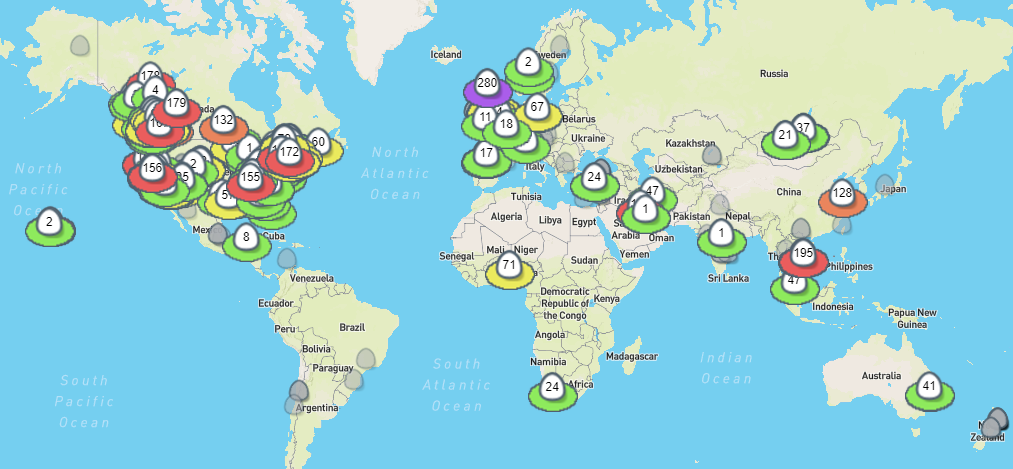
\includegraphics[scale=0.58]{figs/sb_airqualityeggmap.png}
    \caption{Harta senzorilor Egg}
    \label{fig:sb_airqualityeggmap}
\end{figure}

Aplicatiile web si pentru telefon smart ofera posibilitatea de vizualizare a datelor in timp real si a datelor istorice sub forma grafica sau ca valori de sine 
statatoare. De asemenea, aceste date sunt acompaniate de un cod de culori. Fiecare culoare corespunde unui interval de valori al indicelui de calitate al 
aerului (AQI):
\begin{itemize}
	\item Intervalul [0, 50] semnifica o calitate a aerului buna si este reprezentata prin culoarea verde.
	\item Intervalul [51, 100] semnifica o calitate a aerului moderata si este reprezentata prin culoarea galbena.
	\item Intervalul [101, 150] semnifica o calitate a aerului nesanatoasa pentru persoane sensibile si este reprezentata prin culoarea portocaliu.
	\item Intervalul [151, 200] semnifica o calitate a aerului nesanatoasa si este reprezentata prin culoarea rosie.
	\item Intervalul [201, 300] semnifica o calitate a aerului foarte nesanatoasa si este reprezentata prin culoarea mov.
	\item Intervalul [301, 500] semnifica o calitate a aerului riscanta si este reprezentata prin culoarea maro.
\end{itemize}

Procesul de instalare si configurare al unui senzor Egg este realizat prin conectarea acestuia la un calculator si utilizarea unei aplicatii oferita de Air 
Quality Egg. Cu ajutorul acestei aplicatii sunt transmise senzorului informatiile necesare pentru ca acesta sa se conecteze la un router (SSID, parola). De 
asemenea, aplicatia aceasta poate fi utilizata si pentru colectarea metricilor de calitate a aerului prin portul serial in cazul in care nu se doreste conectarea 
acestuia la un router. Senzorul este alimentat de la o sursa de 5V prin cablu USB.

Dupa procesul de instalare senzorul va incepe sa transmita datele colectate in serverul cloud si vor fi disponibile in aplicatiile web si de pe telefonul smart.

Platforma hardware a senzorului utilizeaza controlerul de retea CC3000 de la Texax Instruments pentru realizarea conexiunii Wi-Fi si poate contine senzori pentru 
colectarea metricilor de calitate a aerului prezentate mai jos. Un singur senzor nu poate contine toate aceste metrici, toti senzorii colecteaza metricile pentru 
temperatura, umiditate si presiune barometrica, iar in functie de urmatoarele metrici alease se poate ca altele sa nu mai poate fi integrate in senzor. De exemplu, 
daca se alege colectarea metricilor aditionale CO2, SO2 si NO2, nu mai este permisa adaugarea in senzor si a metricilor O3, H2S sau CO.
\begin{itemize}
	\item Particulele in suspensie OM1.0, PM2.5 si PM10.
	\item Dioxid de Carbon (CO2).
	\item Concentratia Compusilor Organici Volatili Totala (TVOC).
	\item Umiditate.
	\item Temperatura.
	\item Dioxid de sulf (SO2). 
	\item Ozon (O3).
	\item Dioxid de Nitrogen (NO2).
	\item Monoxid de carbon (CO).
	\item Sulfat de Hidrogen (H2S).
\end{itemize}

\subsection{Avantaje}\label{subsec:airqualityegg_avantaje}
\begin{itemize}
	\item Platforma hardware care poate fi personalizata.
	\item Vizualizarea si capabilitatea de analizare a datelor raportate de senzorii Egg din intreaga lume.
	\item Posibilitatea de inlocuire a componentelor senzorului.
\end{itemize}

\section{Solutia PurpleAir}\label{sec:sb_purpleair}
\subsection{Descriere}\label{subsec:sb_purpleair_descriere}
Solutia oferita de compania PurpleAir se concentreaza pe impartasirea datelor colectate cu intreaga lume prin platforma oferita de acestia. Ofera patru variante 
de senzori de calitate a aerului care au capabilitatea de conectare la un server cloud. Trei dintre aceesti senzori sunt destinati pentru spatii inchise, spatii 
deschise sau domeniul industrial, iar al patrulea este destinat doar pentru spatii inchise. Informatiile continute in acest capitol au fost extrase de pe site-ul oficial de 
prezentare al companiei PurpleAir si din manualele de instalare si de depanare puse la dispozitie de acesta \cite{purpleair}.

Senzorii destinati pentru spatii deschise sau domeniul industrial sunt incapsulati intr-o cutie rezistenta la conditiile meteo din spatiile deschise si la 
conditiile extreme din domeniul industrial cum ar fi, temperaturi extreme sau umiditate crescuta. Acestia au capabilitatea de functionare fara conexiune Wi-Fi 
utilizand un card de memorie de maxim 64 GB de pe care datele pot fi extrase prin portul Micro USB. Tot prin portul Micro USB se realizeaza si alimentarea 
acestora cu 5V.

Pentru instalarea senzorului in cazul in care se doreste adaugarea acestuia intr-o retea Wi-Fi este necesara utilizarea unui computer sau a unui telefon smart 
cu capabilitatea de conectare la o retea Wi-Fi. La prima utilizare sau dupa o resetare a senzorului acesta intra in modul AP in care se comporta ca un router cu 
capabilitatea de conectare a unui singur device. Senzorul va aparea in lista de retele Wi-Fi cu denumirea "PurpleAir\_[numele senzorului]". Informatiile despre 
reteaua locala la care se doreste conectarea senzorului, SSID, parola etc, sunt transmise prin conectarea la reteaua creata de senzor si accesara unei pagini 
web de configurare. La finalul procesului de instalare, senzorul va opri reteaua locala creata, se va conecta la routerul despre care a primit informatii 
si va incepe sa transmita date periodic catre serverul din cloud.

Figura \ref{fig:sb_purpleairmap} prezinta harta snezorilor pusa la dispozitie de PurpleAir pentru vizualizarea calitatii aerului din intreaga lume. Pentru 
ca un senzor sa apara pe aceasta harta si pentru ca datele colectate de acesta sa poata fi accesate de orice persoana, senzorul trebuie inregistrat de catre 
utilizator in platforma PurpleAir. 
\begin{figure}[H]
    \centering
    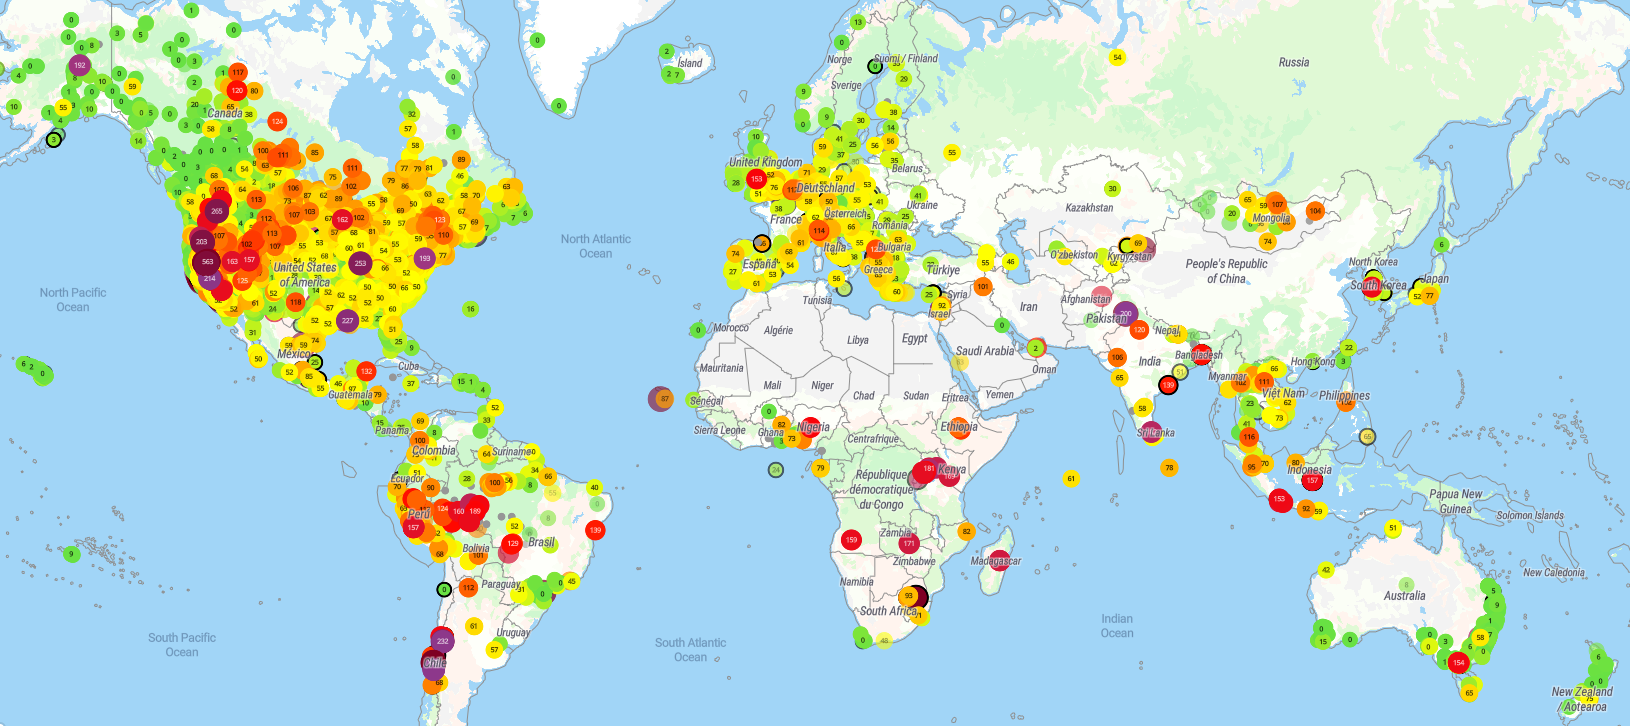
\includegraphics[scale=0.35]{figs/sb_purpleairmap.png}
    \caption{Harta senzorilor PurpleAir}
    \label{fig:sb_purpleairmap}
\end{figure}

In cazul conectarii senzorului la o retea locala fara access la internet, datele colectate de acesta pot fi accesate prin introducerea manuala a unei adrese 
URL in browserul web. Primul pas in aceasta procedura este identificarea IP-ului pe care senzorul la primit la conecarea in reteaua locala. Pentru acest lucru 
este necesara accesarea paginii de configurare a routerului si identificarea manuala, dintr-o lista de IP-uri, a IP-ului specific senzorului. Adresa URL 
introdusa in browserul web reprezinta o cerere HTTP de tip GET al carei raspuns este afisat in pagina web in format JSON.

Metricile de calitate a aerului colectate de senzori sunt:
\begin{itemize}
	\item Particulele in suspensie PM1.0, PM2.5, PM10.
	\item Presiune.
	\item Umiditate.
	\item Temperatura.
	\item Gaze.
\end{itemize}
Pentru colectarea metricilor PM1.0, PM2.5 si PM10 este utilizat senzorul PMS-x0003 de la Plantowner. Fiecare senzor detinut de AirPurple contine doua 
unitati PMS-x0003 pentru redundanta, iar pentru colectarea metricilor de presiune, temperatura, umiditate si gaze este utilizat senzorul BME688 de la BOSH. Pentru 
conexiunea Wi-Fi, snezorii utilizeaza controlerul de retea ESP-WROOM-02D de la Espressif Systems. Toti senzorii utilizati in acest paragraf sunt destinati pentru 
utilizarea in domeniul industrial avand intervalul de temperatura de functionare [-40, +85] grade celsius.

Metricile de presiune, umiditate, temperatura si gaze sunt utilizate pentru calcularea indicelui de calitate al aerului (AQI) dupa standardul creat de Agentia de 
Protectie a Mediului din Statele Unite.

PurpleAir este integrat cu platforma guvernamentala AirNow care ofera o harta, asemanatoare cu cea oferita de PurpleAir, unde pot fi observate datele colectate 
de senzori de la mai multe companii printre care si PurpleAir.

\subsection{Avantaje}\label{subsec:sb_purpleair_avantaje}
\begin{itemize}
	\item Platforma software pentru vizualizarea senzorilor si a calitatii aerului din intreaga lume.
	\item Posibilitatea de inlocuire a componentelor senzorilor.
\end{itemize}
\subsection{Dezavantaje}\label{subsec:sb_purpleair_dezavantaje}
\begin{itemize}
	\item Afisarea datelor catre utilizator in format JSON in anumite moduri de functionare, un format greu de citit de catre utilizator.
\end{itemize} % \chapter{Studiu Bibliografic}

\chapter{Analiză și fundamentare teoretică}
\label{ch:analysis}
\pagestyle{fancy}

\section{Protocoale de comunicatie}\label{sec:protocols}
\subsection{TCP/IP}\label{subsec:tcpip}
TCP/IP este o stiva de comunicatie, un protocol, care sta la baza internetului si a interconectivitatii dispozitivelor. Majoritatea dispozitivelor 
care suporta conexiunea la interent, de exemplu, telefoane, calculatoare personale etc, gestioneaza aceasta stiva de comunicatie. Implementeaza o arhitectura 
pe 5 nivele unde fiecare nivel poate implementa diferite protocoale specifice si este constient doar de nivelele care il inconjoara, nivelul superior 
si cel inferior lui. 

Figura \ref{fig:TCPIP_Layers} prezinta nivelele stivei de comunicatie TCP/IP in contextul a doua dispozitive conectate la un router.
\begin{figure}[H]
    \centering
    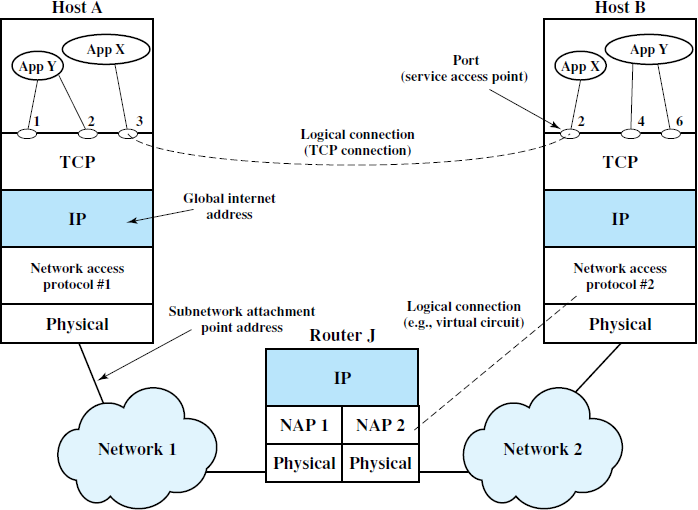
\includegraphics[scale=0.8]{figs/TCPIP_Layers.png}
    \caption{Stiva de comunicare TCP/IP \cite{williamStallings}}
    \label{fig:TCPIP_Layers}
\end{figure}

Host A si Host B reprezinta doua dispozitive conectate la un router care implementeaza stiva TCP/IP. De exemplu, un calculator personal si un telefon.

Nivelul aplicatiei, reprezentat in figura prin App X si App Y, contine protocoale de comunicatie de nivel inalt, cum ar fi protocolul HTTP, FTP, MQTT etc. 
Acest nivel trimite catre nivelul TCP informatii precum, adresa ip si portul dispozitivului destinatie.

Nivelul transport, reprezentat in figura prin TCP, Are rolul de a se asigura ca mesajele trimise de aplicatiile de la nivelul precedent ajung la destinatie 
fara erori si in ordinea in care au fost trimise. De asemenea, la acest nivel se gestioneaza si porturile aplicatiilor. 

Nivelul internet protocol, reprezentat in figura prin IP, se ocupa de transmisia datelor prin mai multe retele pana la destinatia finala. La acest nivel 
mesajului i se ataseaza adresa IP a destinatiei primita de la nivelul TCP. Astfel mesajul poate fi transmis prin mai multe retele pana atinge dispozitivul 
destinatie.

Nivelul de acces retea, reprezentat in figura prin Network access protocol \#1, se ocupa de transmisia datelor catre urmatorul dispozitiv din sub-reteaua.
lui. In cazul schemei, urmatorul dispozitiv din retea este router-ul. Nu este responsabil de destinatia finala a mesajului.

Nivelul fizic, reprezentat in figura prin Physical, se ocupa de transformarea mesajului primit de la nivelul precedent in unde radio, in cazul 
comunicatiei fara fir, sau in semnal electric sau luminos, in cazul comunicatiei pe fir si de transmisia acestuia prin retea. 

Routerul, reprezentat in figura prin Router J, implementeaza nivelele de jos ale stivei, IP, Network Access protocol, si Physical. Implementeaza doar aceste 
trei nivele din stiva, deoarece rolul lui este de a crea o legatura intre doua retele. Un mesaj primit de la un dispozitiv din reteaua 1 va fi decodat pana 
la nivelul IP, apoi recodificat cu urmatoarea destinatie si transmis.

Fiecare nivel adauga la mesajul original trimis de nivelul aplicatiei un antet si in unele cazuri si un subsol. Subsolul reprezinta un cod de verificare a 
erorilor, cum ar fi CRC, iar antetul reprezinta informatii specifice rolului nivelului de care este adaugat. La raceptia unui mesaj calea acestuia este inversa, 
de la nivelul Physical catre nivelul Application.

Termenul Socket reprezinta o pereche (Host, Port) care identifica unic un dispozitiv in tot internetul. Perechea (Host, Port) este formata din adresa globala
a unui dispozitiv si portul pe care acesta comunica. De exemplu, la crearea unei conexiuni intre doua dispozitive, initiatorul conexiunii trebuie sa cunoasca si 
sa adauge in mesajul trimis adresa globala in internet a dispozitivului destinatie si portul pe care acesta asculta. Socket-ul este utilizat la crearea unei 
conexiuni intre doua aplicatii.

\subsection{HTTP}\label{sec:http}
Protocolul de comunicatie HTTP reprezinta standardul pentru comunicarea documentelor prin internet. Acesta este utilizat cu preponderenta pentru obinerea paginilor 
web de la un server web. Este un model de comunicatie client-server, unu la unu, care defineste cum sunt formatate informatiile si trimise de catre client si 
cum trebuie sa raspuna server-ul la acestea.

Modelul de comunicatie este de tipul cerere-raspuns. Clientul trimite o adresa URL catre server, apoi asteapta un raspuns. Serverul primeste adresa, 
identifica unic un set de date, de exemplu, o pagina web sau o imagine, pe baza adresei URL, apoi returneaza un raspuns care contine informatiile cerute 
de client. Este un protocol de comunicatie sincron, deoarece se asteapta raspunsul la crerere, spre deosebire de alte protocoale de comunicatie, 
de exemplu, MQTT, unde se trimit date catre server fara a se astepta un raspuns la acestea.

HTTP este utilizat pentru tranzactionarile de date mari, neavand o limita superioara de dimensiune a pachetului. Totusi dimensiunile utilizate in mod 
uzual sun relativ mici din cauza timpului de raspuns care creste odata cu dimensiunea resursei.

In stiva de comunicare a protocolului TCP/IP, HTTP se afla in nivelul cel mai inatlt, si anume, nivelul aplicatiei. Acest lucru inseamna ca HTTP nu se 
ocupa de transportul efectiv al mesajelor printr-o retea, ci doar defineste un limbaj comun pentru arhitectura de comunicatie client-server.  

Antetul unui mesaj este bazat pe text, insemnand ca particularitatile mesajelor sunt reprezentate prin cuvinte intuitive spre deosebire de MQTT unde 
particularitatile sunt reprezentate prin biti sau set de biti. Mai jos sunt prezentate cele mai uzuale astfel de proprietati:
\begin{itemize}
	\item Content-Type - specifica in ce format sunt codate datele cuprinse in corpul mesajului. Valoarea acestuia poate fi JSON, XML etc.
	\item Content-Length - specifica dimensiunea corpului mesajului. Cum s-a precizat si mai sus, nu exista o valoare maxima petru acest camp, dar 
	in mod uzual nu depaseste 256MB.
    \item Accept - formate ale datelor care sunt acceptate de catre client ca raspuns. De exemplu, un client poate cere unui server un set de imagini si 
    prin acest camp informeaza server-ul sa-i ofere doar imagini in format jpeg.
    \item User-Agent - utilizat de client pentru a specifica informtii despre el insusi, de exemplu, tipul aplicatiei, versiunea etc.
    \item Connection - poate lua doua valori, "keep-alive" si "close". Este utilizat de client pentru a specifica daca doreste sa fie incheiata conexiunea 
    dupa returnarea raspunsului. "keep-alive" va informa serverul ca actuala conexiune va ramane deschisa pentru un nou request, iar "close" il va 
    informa ca va fi incheata conexiunea.
\end{itemize}

\

O metoda HTTP reprezinta o actiune pe care un client o trimite unui server pentru a fi executata. Cele mai comune metode HTTP sunt:
\begin{itemize}
	\item GET - prin aceasta metoda clientul cere o resursa server-ului
	\item POST - prin aceasta metoda clientul trimite un set de date catre server pentru a modifica o resursa sau pentru a salva o resursa noua. Daca 
	adresa URL contine o resursa care nu exista deja, cererea va returna codul de eroare 404.
	\item PUT -  prin aceasta metoda clientul trimite un set de date catre server pentru a suprascrie o resursa sau pentru a crea o resursa noua. Daca 
    este trimis un URL cu o resursa care nu exista, aceasta va fi creata.
	\item DELETE - prin aceasta metoda clientul sterge o resursa de pe server.
\end{itemize}

\

O adresa URL este compusa din trei parti principale:
\begin{itemize}
	\item Protocolul utilizat pentru extragerea resursei. In general acesta este HTTP si este de forma "http://".
	\item Adresa serverului sau locatia serverului. De exempu, www.universitatea\_tehnica.ro.
	\item Identificatorul unic al resursei. De exemplu, /clientID/1 sau /index.html.
\end{itemize}

\

Codul de status este un cod returnat de server in raspuns care instiinteaza clientul de statusul executiei cererii. Sunt foarte multe coduri de eroare 
impartite pe categorii de erori, fiecare reprezentand o eroare diferita. Mai jos sunt enumerate cele mai utilizate coduri de eroare:
\begin{itemize}
	\item 200 - Success. Serverul instiinteaza clientul ca actiunea a fost executata cu success.
	\item 400 - Bad Request. Serverul nu accepta cererea clientului, deoarece aceasta este eronata. 
	\item 403 - Forbidden. Este trimisa de server atunci cand clientul nu are autoritatea sa acceseze o anumita resursa.
	\item 404 - Not found. Resursa ceruta de client nu poate fi gasita. 
\end{itemize}

\

\subsection{MQTT}\label{sec:mqtt}
Standardul MQTT defineste un set de reguli, un limbaj, pe care doua sau mai multe entitati trebuie sa il respecte pentru a putea schimba mesaje intre 
ele. Entitatile acestuia sunt clientii si un server, numit Broker. Este un protocol pentru transmiterea mesajelor prin internet care necesita resurse reduse si 
utilizeaza un model de comunicatie de tip publica/aboneaza. In mod uzual opereaza impreuna cu stiva de comunicatie TCP/IP, dar poate fi integrat si cu alte 
standarde, cum ar fi ZigBee sau LoRa. Acest protocol este foarte utilizat in domeniul Internetul Lucrurilor fiind potrivit pentru 
senzorii cu capacitati de procesare reduse si oferind un grad inalt de scalabilitate prin structura de functionare a acestuia. In urmatoarele paragrafe 
din acest capitol vom analiza caracteristicile cheie ale acestui protocol.

Broker-ul este un server, o unitate centrala, specializat pe receptia mesajelor de la clienti si retransmisia acestora catre clientii interesati de 
tipul de mesaj respectiv. Acesta poate fi vizualizat ca o unitate de decuplare, deoarece clientii nu comunica direct intre ei, ci prin acest manager de 
mesaje. Comunicarea este de tip asincrona, calea unei tranzactii porneste de la client si se opreste la Broker, deci o tranzactie nu implica doi clienti 
in acelasi timp. 

Modelul de comunicatie publica/aboneaza imparte clientii in doua categorii, clienti care publica, transmit, mesaje catre Broker si clienti care se aboneaza
la Broker pentru a receptiona mesajele publicate. Clientii pot avea ambele roluri, si de publicatori si de abonati, pastrand rolurile disjuncte. Astfel ca 
un client care are ambele roluri va publica periodic un set de date si in acelasi timp va fi abonat la Broker pentru receptia de mesaje de la unul sau mai 
multi clienti. In mod uzual aceste roluri pot fi impartite in doua categorii, rol principal si rol secundar. In cazul uni senzor, rolul principal este 
de a publica date despre mediul inconjurator, iar rolul secundar este de abonare pentru a receptiona modificari ale configuratiilor acestuia, de exemplu, 
perioada la care se face publicarea. In cazul unui client smartphone sau pagina web, rolul principal este de abonat pentru a receptiona metricile de la senzori, 
iar rolul secundar este de publicator pentru transmisia de configuratii catre senzor.

Figura \ref{fig:MQTTBrokerArchitecture} prezinta arhitectura publica/aboneaza a protocolului de comunicatie MQTT. Fiecare modul prezentat in figura este 
descris in paragrafele de mai sus.
\begin{figure}[H]
    \centering
    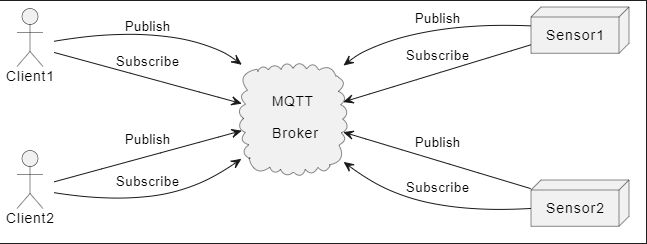
\includegraphics[scale=0.8]{figs/MQTTBrokerArchitecture.png}
    \caption{Arhitectura publica/aboneaza a protocolului MQTT}
    \label{fig:MQTTBrokerArchitecture}
\end{figure}

Subeictul mesajelor, denumit topic in standard \cite{mqttstandard}, reprezinta o serie de cuvinte structurate pe nivele care descriu intr-un mod succint datele mesajului. 
Aceste cuvinte sunt separate prin caracterul special "/", denumit si separator de nivel, si au rolul de a filtra mesajele trimise catre clienti. 
De exemplu, Un senzor transmite un mesaj care contine date de temperatura catre Broker sub subiectul "IDsenzor/citiri/temperatura". 
Broker-ul va redirectiona acest mesaj doar catre clientii care sunt abonati pentru receptia de mesaje care au subiectul "IDsenzor/citiri/temperatura".

Structura unui mesaj MQTT este de tip binar, fiecare bit sau grupare de biti indentifica un tip de mesaj sau diferite proprietati, in comparatie cu alte 
protocoale de comunicatie care utilizeaza un format bazat pe text, unde tipurile de mesaje sau proprietatile sunt identificate prin text, de exemplu,
protocolul de comunicatie HTTP. Principalul avantaj al formatului de tip binar este dimensiunea scazuta a pachetului. Tabelul \ref{tab:StructuraMesajMQTT} 
contine o prezentare generala a acestui pachet unde:
\begin{itemize}
	\item Control Field - reprezinta octetul de control al pachetului si este impartit in doua zone:
    \begin{itemize}
        \item Tipul pachetului in primii 4 biti
        \item Semnale pentru activarea sau dezactivarea unor proprietati
    \end{itemize}
	\item Remaining Length - poate avea o lungime cuprinsa intre 1 si 4 octeti si reprezinta lungimea ramasa in pachet, adica lungimea campurilor Variable Header 
    si Payload
	\item Variable Header - are o lungime variabila care este cuprinsa in campul precedent. Acest camp difera in functie de tipul mesajului, de exemplu, in 
	cazul mesajului de publicare a datelor acest camp contine subiectul.
	\item Payload - are o lungime variabila care este cuprinsa in campul Remaining Length si reprezinta partea utila a mesajului, de exemplu, datele citite de 
	la senzor.
\end{itemize}

\begin{table}[ht]
    \caption{Structura mesaj MQTT}
    \centering                          % tabel centrat
    \begin{tabular}{|c|c|c|c|}          % 4 coloane centrate
        \hline
        1 B & 1-4 B & x B & x B \\ [0.5ex]   % inserare tabel
        %heading
        \hline                              % linie orizontal simpla
        Control Field & Remaining Length & Variable Header & Payload \\               % corpul tabelului
        \hline
    \end{tabular}
    % titlul tabelului
    \label{tab:StructuraMesajMQTT}                % eticheta folosita pentru referirea tabelului in text; referirea in text se va face cu \ref{table:nonlin}
\end{table}

Tranzactia reprezinta un schimb de mesaje intre un client si Broker si are o structura de tip cerere si confirmare. Cererea este un mesaj care contine informatii 
utile, de exemplu, datele unui senzor sau datele necesare conectarii la Broker, iar confirmarea este un mesaj prin care Borker-ul instiinteaza clientul ca cererea 
lui a fost inregistrata. Acestea din urma sunt transmise si in caz de eroare si in caz de success, iar acest lucru este semnalat in campul "Variable Header" 
prezentat in tabelul \ref{tab:StructuraMesajMQTT}. Protocolul MQTT contine mai multe tipuri de mesaje impartite pe cele doua categorii prezentate mai sus dintre 
care cele mai importante sunt prezentate in cele ce urmeaza:
\begin{itemize}
    \item CONNECT - acest pachet este trimis de catre client pentru a realiza o conexiune cu Broker-ul.
    \item CONNACK - acest pachet este trimis de catre Broker si reprezinta raspunsul pentru mesajul CONNECT si are rolul de a confirma realizarea conexiunii.
    \item PUBLISH - acest pachet este trimis de catre client si contine subiectul si datele utile.
    \item PUBACK - acest pachet este trimis de catre Broker ca raspuns la mesajul PUBLISH.
    \item SUBSCRIBE - acest pachet este trimis de catre client si reprezinta cererea de abonare la un anumit subiect. Subiectul este continut in pachet.
    \item SUBACK - acest pachet este trimis de catre Broker si reprezinta confirmarea subscriptiei clientului.
\end{itemize}

Conexiunea dintre client si Broker se realizeaza la cererea clientului print trimiterea unui mesaj specific. Acest tip de mesaj contine un camp special 
denumit "keep alive" prin care clientul informeaza Broker-ul de durata de viata a conexiunii dintre acestia. Clientul poate alege inchiderea conexiunii 
cu Broker-ul dupa fiecare mesaj de publicare a datelor cu scopul de a intra intr-un mod de consum de putere redus pana la urmatoarea perioada de 
publicare. Salvarea energiei aduce cu sine cresterea numarului de mesaje interschimbate intre client si Broker, dar aduce avantaje in durata de viata 
a bateriei. 

\subsection{Wi-Fi}\label{sec:wifi}
Wi-Fi reprezinta un set de protocoale de comunicatie fara fir bazate pe standardul IEEE 802.11. In stiva TCP/IP acesta este implementat in ultimele 2 nivele, 
Network Addressing (MAC) si Physical. Acesta permite crearea unei retele locale de dispozitive interconectate fara cabluri fizice.

O retea Wi-Fi uzuala este formata din doua tipuri de dispozitive, statii de baza si statii client. Statiile de baza reprezinta punctul central al unei retele Wi-Fi 
si gestioneaza conexiunea si distribuirea mesajelor intre statiile client connectate la aceasta. Statiile client nu pot comunica direct intre ele, ci prin 
intermediul statiei de baza. Acest tip de retea este utilizat cu preponderenta pentru a oferi statiilor client conexiune la internet. Pentru acest lucru 
statia de baza este connectata la un modem care la randul lui este conectat la reteaua furnizorului de internet.

Un alt tip de retea Wi-Fi, mai putin utilizata, este reteaua punct la punct si este formata doar din statii client interconectate intre ele in mod direct. 
Acest tip de retea utilizeaza un protocol numit Wi-Fi Direct si este utilizata pentru conexiuni si tranzactii de date intre doua statii client.

Nivelul Physical are rolul de a codifica si decodifica semnalele digitale in semnale radio in benzile de frecventa 2.4GHz si 5GHz. Aceste benzi fac parte din 
din benzile de frecventa ISM alocate pentru utilizarea in domeniile industrial, stiintific si medical. Petru codificarea si decodificarea datelor 
sunt utilizate mai multe scheme de modulatie, din care, schema de modulatie OFDM este utilizata cu preponderenta. 

Banda de frecventa 2.4GHz reprezinta intervarul de frecvente cuprins intre 2.4GHz si 2.5GHz. Acest interval de 100 MHz este impartit in 14 canale partial 
suprapuse. Fiecare canal are o latime de banda de 22 MHz. Majoritatea dispozitivelor ofera utilizatorului posibilitatea de a schimba canalul de comunicatie 
cu scopul imbunatatirii vitezei. O viteza mai buna este obtinuta prin scaderea interferentei dintre dispozitivele dintr-o retea, acest lucru fiind obtinut 
prin imprastierea dispozitivelor pe cele 14 canale. 

Figura \ref{fig:2400MHz_channels} prezinta modul in care banda de frecventa 2.4GHz este impartita in cele 14 canale. Fiecare canal are notat deasupra lui 
numarul si centrul frecventei acestuia.
\begin{figure}[H]
    \centering
    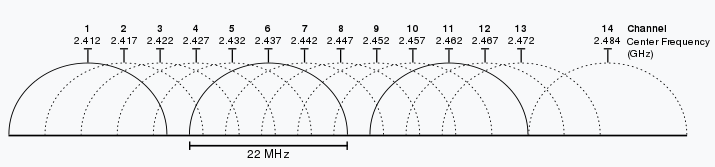
\includegraphics[scale=0.8]{figs/2400MHz_channels.png}
    \caption{Canalele de comunicatie in banda de frecventa 2.4GHz \cite{wifichannels}}
    \label{fig:2400MHz_channels}
\end{figure}

Nivelul MAC are rolul de a gestiona si mentine comunicatia intre o statie client si o statie de baza dintr-o retea locala. Acesta este responsabil de 
transmiterea pachetului de la statia client catre statia de baza, de retransmiterea pachetului in cazul in care acesta nu a fost receptionat de catre 
statia de baza, de evitare a coliziunilor cu alte dispozitive din retea etc.

Conexiunea dintre o statie client si o statie de baza se poate realiza in doua moduri, activ sau pasiv. In modul activ, statia client transmite pachete 
care contin informatii despre capabilitatile lui, iar statiile de baza raspund la aceste pachete cu numele retelei si alte informatii legate de retea. 
In modul pasiv, statia de baza transmite periodic pachete prin care isi anunta prezenta, iar statiile client intra in receptie pe fiecare canal cu scopul 
de a receptiona un astfel de frame. Dupa acest prim pas, urmeaza un schimb de pachete prin care se realizeaza conexiunea dintre statia client si statia de baza.

Acest protocol, in comparatie cu un protocol pe fir, faciliteaza instalarea unei retele locale prin inlaturarea necesitatii cablurilor si a rutarii acestora 
si mobilitatea dispozitivelor din retea fiind permisa deplasarea dispozitivelor in raza de acoperire a statiei de baza. De asemenea, principalele dezavantaje 
ale acestuia sunt interferenta dintre dispozitivele din retea si raza de acoperire a statiei de baza.

\subsection{SPI}\label{sec:spi}
SPI, Serial Peripheral Interface, este un protocol de comunicatie seriala si sincrona. Arhitectura acestuia este formata din dispozitive care pot avea 2 
roluri, master sau slave. Intr-o arhitectura SPI poate exista un singur dispozitiv master si unul sau mai multe dispozitive slave. Acest protocol a fost 
proiectat pentru communicatia dintre un microcontroller, dispozitivul master, si perifericele acestuia, dispozitivele slave. 

Liniile de semnal utilizate in protocolul SPI sunt:
\begin{itemize}
    \item SS (Slave Select) este un semnal controlat de dispozitivul master prin care activeaza dispozitivul slave pentru o transmisie de date.
    \item SCLK (Serial Clock) este un semnal generat de dispozitivul master pentru sincronizarea cu dispozitivul slave in timpul unei transmisii de date.
    \item MOSI (Master Out Slave In) este semnalul de date prin care dispozitivul master transmite date dispozitivului slave. Aceasta linie de semnal 
    poate sa lipseasca in anumite moduri de comunicatie.
    \item MISO (Master In Salve Out) este semnalul de date prin care dispozitivul slave transmite date dispozitivului master. Aceasta linie de semnal 
    poate sa lipseasca in anumite moduri de comunicatie.
\end{itemize}

\

Comunucatia dintre doua dispozitive, master si slave, se poate realizeaza prin 3 sau 4 linii de semnal. Modul de communicatie cu 3 linii de semnal se poate 
numi Simplex sau Half-Duplex, iar cel cu 4 linii de semnal Full-Duplex:
\begin{itemize}
    \item Simplex reprezinta modul de comunicatie in care doar dispozitivul master poate transmite date catre unul sau mai multe dispozitive slave. Liniile 
    de semnal utilizate sunt SS, SCLK si MOSI.
    \item Half-Duplex reprezinta modul de comunicatie in care este utilizata o singura linie de date, comuna intre un dispozitiv master si unul sau mai multe 
    dispozitive slave, pentru transmisia de date de la master catre slave sau de la slave catre master. Un singur dispozitiv poate transmite la un moment dat. 
    Liniile de semnal utilizate sunt SS, SCLK si MOSI/MISO.
    \item Full-Duplex reprezinta modul de comunicatie cel mai utilizat. Acesta utilizeaza 2 linii de date pentru tranzactionarea intre un dispozitiv master 
    si unul sau mai multe dispozitive slave. O linie este utilizata pentru transmisia de date de la master catre slave si una pentru transmisia datelor de 
    la slave catre master. Dispozitivela master si slave pot transmite date simultan. Liniile de semnal utilizate sunt SS, SCLK, MOSI si MISO.    
\end{itemize}

Figura \ref{fig:SPIMasterSlave} prezinta modul de comunicatie Full-Duplex al protocolului SPI dintre un dispozitiv master si doua dispozitive Slave.
\begin{figure}[H]
    \centering
    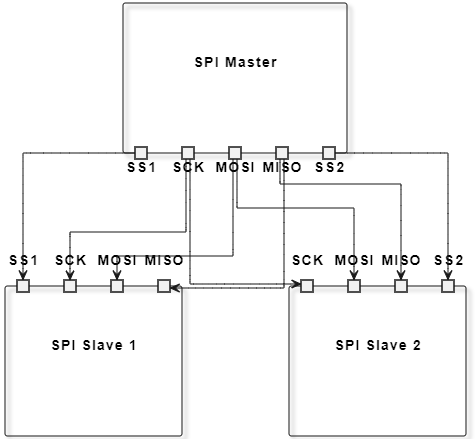
\includegraphics[scale=0.8]{figs/SPIMasterSlave.png}
    \caption{Arhitectura protocolului SPI Full-Duplex}
    \label{fig:SPIMasterSlave}
\end{figure}

Intr-o arhitectura SPI in care exista mai multe dispozitive slave, dispozitivul master are o line de semnal SS specifica fiecarui dispozitiv slave, iar liniile 
de semnal SCK, MOSI si MISO sunt comune. Astfel, atunci cand dispozitivul master initiaza o tranzactie cu un dispozitiv slave, activeaza linia de semnal SS 
legata la acel slave, celelalte dispozitive slave ramanand inactive.

Un alt mod, mai putin utilizat, in care liniile de semnal pot fi legate intre un dispozitiv master si mai multe dispozitive slave este prin inlantuirea 
dispozitivelor slave. Astfel, dispozitivul master are o singura linie de semnal SS comuna pentru toate dispozitivele slave, linia de semnal MOSI este legata 
la primul dispozitiv slave din lant, iar linia MISO este legta la ultimul dispozitiv slave din lant. La initierea unei tranzactii, dispozitivul master activeaza 
toate dispozitivele slave, transmite date catre primul dispozitiv slave din lant, iar fiecare slave din lant redirectioneaza datele catre urmatorul. Atunci cand 
datele transmise de master ajung la dispozitivul slave cu care se doreste comunicarea, acesta proceseaza datele si redirectioneaza un mesaj nou catre urmatorul 
slave. Acest mod de comunicare este utilizat doar in cazul in care nu este posibila rutarea unui semnal SS catre fiecare dispozitiv slave.

Protocolul SPI permite gestionarea polaritatii si a fazei semnalului de ceas pentru prelevarea datelor. Dispozitivul master este responsabil de utilizarea 
polaritatii si a fazei suportate de dispozitivul slave. Tabelul \ref{tab:spiPolPhase} prezinta cele 4 moduri in care datele pot fi prelevate.
\begin{table}[ht]
    \caption{Polaritateaa si faza semnalului de ceas}
    \centering   % tabel centrat
    \renewcommand{\arraystretch}{2.2}
    \begin{tabular}{|c|c|c|}          % 4 coloane centrate
        \hline
        Polaritate & Faza & Descriere \\ [0.5ex]   % inserare tabel
        %heading
        \hline                          % linie orizontal simpla
        0 & 0 & \parbox{280pt}{SCLK are valoarea 0 logic cand este inactiva, iar datele sunt prelevate pe frontul crescator}\\ 
        0 & 1 & \parbox{280pt}{SCLK are valoarea 0 logic cand este inactiva, iar datele sunt prelevate pe frontul descrescator}\\ 
        1 & 0 & \parbox{280pt}{SCLK are valoarea 1 logic cand este inactiva, iar datele sunt prelevate pe frontul descrescator}\\ 
        1 & 1 & \parbox{280pt}{SCLK are valoarea 1 logic cand este inactiva, iar datele sunt prelevate pe frontul crescator}\\ 
        \hline
    \end{tabular}
    % titlul tabelului
    \label{tab:spiPolPhase}                % eticheta folosita pentru referirea tabelului in text; referirea in text se va face cu \ref{table:nonlin}
\end{table}

Figura \ref{fig:SPITimingDiagram} prezinta in detaliu modul in care sunt tranzactionate date intre un dispozitiv master si unul slave. Este prezentat modul de 
comunicatie Full-Duplex cu semnalul de ceas avand caracteristicile de polaritate si faza 0 si 0, adica semnalul SCLK are valoare 0 in modul inactiv, iar datele 
sunt prelevate pe frontul crescator.
\begin{figure}[H]
    \centering
    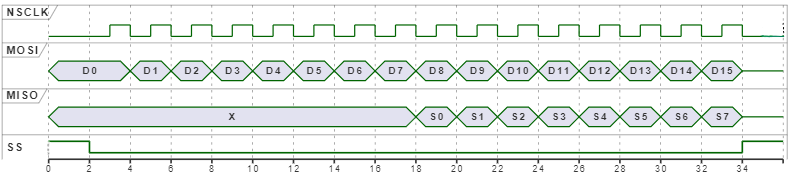
\includegraphics[scale=0.75]{figs/SPITimingDiagram.png}
    \caption{Diagrama de timp a comunicatiei SPI}
    \label{fig:SPITimingDiagram}
\end{figure}

Datele sunt transmise intre un dispozitiv master si unul slave bit cu bit. Dispozitivul master activeaza linia SS prin tranzitia din 1 logic in 0 logic, 
apoi seteaza linia MOSI in conformitate cu primul bit din secventa de biti care urmeaza a fi tranzactionata si genereaza semnalul de ceas. Dupa ce ultimul 
bit a fost transmis, dispozitivul master mentine semnalul de ceas in 1 logic sau in 0 logic in functie de setarea polaritatii, iar apoi dezactiveaza linia 
SS prin tranzitia din 0 logic in 1 logic. De exemplu, in cazul in care semnalul de ceas are caracteristicile de polaritate si faza 0 si 0, pe frontul 
crescator al semnalului de ceas dispozitivul slave citeste starea liniei de semnal MOSI, 1 logic sau 0 logic, iar pe frontul descrescator dispozitivul master 
schimba sau mentine starea liniei conform cu urmatorul bit care urmeaza a fi transmis. In acelasi timp, dispozitivul slave poate tranzitiona linia de date MISO 
in conformitate cu secventa de biti pe care acesta doreste sa o trimita dispozitivului master.

Viteaza de transmisie a acestui protocol este foarte mare in comparatie cu alte protocoale de comunicatie asemanatoare, cum ar fi I2C. Nu ofera un mechanism 
de verificare a erorilor sau de instiintare ca datele au fost receptionate cu success de cealalta parte. Aceste doua dezavantaje pot fi intampinate prin 
utilizarea unui algoritm de verificare a integritatii datelor si a unui mecanism de tip cerere raspuns.

\subsection{I2C}\label{sec:i2c}
I2C este un protocol de comunicatie seriala creat pentru comunicatia dintre un microcontroler si unul sau mai multe periferice ale acestuia. Este un 
protocol sincron, are o arhitectura de tip master slave si necesita doar doua linii de semnal pentru tranzactionarea de date. 

Acest protocol identifica fiecare dispozitiv conectat la magistrala printr-o adresa unica, spre deosebire de alte protocoale precum SPI care necesita cate o 
linie de semnal pentru fiecare dispozitiv sau o inlantuire a dispozitivelor. De asemenea, utilizeaza doar 2 linii de semnal indiferent de numarul de dispozitive 
conectate la magistrala.

Liniile de semnal utilizate sunt numite SDA si SCL, linia de date si respectiv linia de ceas. Acestea sunt bidirectionale, insemnand ca ambele dispozitive 
care participa intr-o tranzactie au control asupra lor. Semnalul de ceas este generat de dispozitivul master, dar dispozitivul slave are capacitatea de a 
forta linia in stare inactiva in cazul in care nu este pregatit pentru a receptiona sau transmite date. De exemplu, dispozitivul slave nu a terminat de 
procesat o sarcina si forteaza linia de ceas in stare inactiva pentru a anunta dispozitivul master sa nu trimita urmatoarele date. Cand sarcina este finalizata, 
dispozitivul slave elibereaza linia de ceas, iar tranzactia datelor isi reia cursul.

Ofera capabilitatea mai multor dispozitive master conectate la aceeasi magistrala. Doar un dispozitiv master poate controla magistrala la un moment dat. 
Decizia de control este luata prin verificarea liniilor magistralei, daca acestea sunt inactive, au valoarea 1 logic, magistrala este libera pentru un transfer,
iar daca acestea sunt ocupate inseamna ca exista o tranzactie in curs de procesare initiata de un alt dispozitiv master de pe magistrala. Pentru a detecta 
corect daca magistrala este libera sau nu, verificarea liniilor trebuie efectuata pentru cel putin o perioada de ceas, deoarece liniile SCL si SDA pot avea 
valoarea 1 logic simultan pentru o jumatate din perioada de ceas.

Figura \ref{fig:I2CBus} prezinta un exemplu de magistrala I2C cu 6 dispozitive conectate. Microcontroller A si Microcontroller B reprezinta dispozitivele master, 
iar celelalte reprezinta dispozitive slave, ecran LCD, convertor din semnal analogic in semnal digital etc.
\begin{figure}[H]
    \centering
    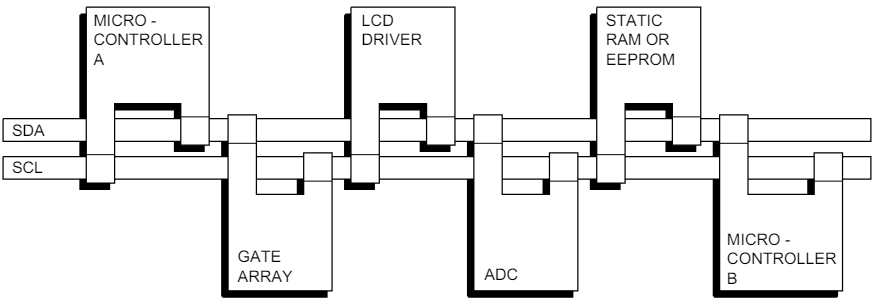
\includegraphics[scale=0.68]{figs/I2CBus.png}
    \caption{Exemplu de magistrala I2C \cite{i2ctutorial}}
    \label{fig:I2CBus}
\end{figure}

Un transfer de date pe magistrala I2C este efectuat in mai multe etape, prima etapa dupa verificarea disponibilitatii magistralei este transmisia unei conditii 
de start. Aceasta conditie este reprezentata de tranzitia din 1 logic in 0 logic a liniei SDA in timp ce linia SCL este in 1 logic si informeaza dispozitivele 
legate la magistrala ca o noua tranzactie este initiata.

A doua etapa este reprezentata de transmisia primului octet care contine adresa dispozitivului slave cu care se va efectua transferul de date pe primii 7 biti si 
a bitului care indica o citire sau o scriere. Toate dispozitivele conectate la magistrala I2C vor receptiona acest octet si il vor compara cu adresa proprie. 
Dispozitivul care este identificat de adresa transmisa va confirma receptia acesteia.

Fiecare octet transmis de un dispozitiv este confirmat sau negat de catre dispozitivul care l-a receptionat. Dispozitivul master ofera un al 9-lea semnal de ceas 
dispozitivului receptor pentru aceasta confirmare. In cazul receptionarii cu success, dispozitivul receptor va mentine linia de date SDA in 0 logic pentru cea de-a 
9-a perioada de ceas (ACK), iar in cazul receptionarii eronate, acesta va mentine linia in 1 logic (NACK).

A treia etapa este reprezentata de transmisia datelor octet cu octet. In cazul unei citiri, dispozitivul master va genera semnalul de ceas, iar dispozitivul slave 
va pune primul octet de date pe linia SDA, urmand apoi al 9-lea puls de ceas prin care dispozitivul master va confirma receptia. In cazul unei scrieri, dispozitivul 
master va genera semnalul de ceas si va pune primul octet de date pe linia SDA, iar dispozitivul slave va confirma receptia acestora.

A patra etapa este transmisia conditiei de stop. Aceasta conditie este reprezentata prin tranzitia liniei de date din o logic in 1 logic  in timp ce linia 
de ceas este in 1 logic. Aceasta conditie reprezinta finalul unei tranzactii intre un dispozitiv master si unul slave.

Pentru cresterea numarului de dispozitive care pot fi conectate la o magistrala si pentru a evita coliziunea de adrese, protocolul I2C ofera capabilitatea 
de a utiliza adrese pe 10 biti. Acest lucru inseamna ca adresarea se va face in primii doi octeti transmisi de dispozitivul master pe magistrala. Primul octet 
contine biti de identificare a tipului de adresare si partea mai semnificativa din adresa, iar al doilea octet contine partea mai putin semnificativa a adresei.

Figura \ref{fig:I2CCompleteDataTransfer} prezinta etapele unei tranzactionari de date intre un dispozitiv master si unul slave.
\begin{figure}[H]
    \centering
    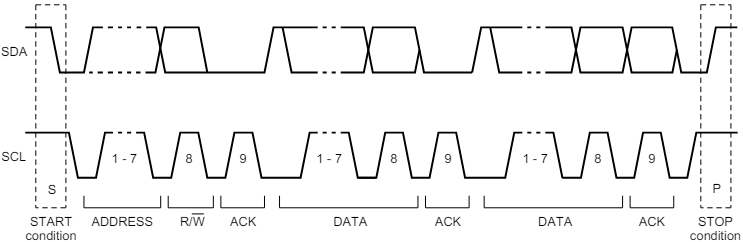
\includegraphics[scale=0.75]{figs/I2CCompleteDataTransfer.png}
    \caption{Exemplu de tranzactie I2C intre un dispozitiv master si unul slave \cite{i2ctutorial}}
    \label{fig:I2CCompleteDataTransfer}
\end{figure}

Pe durata unei transmisii, dispozitivul master sau cel slave poate in orice moment, chiar si in mijlocul transferului unui octet, sa forteze linia de ceas SCL in 
0 logic pentru a opri temporar tranzactia de date. Un exemplu de moment in care un dispozitiv efectueaza aceasta operatie este cand in mijlocul unui transfer 
de date acesta este intrerupt de o rutina interna sau de un alt periferic cu prioritate mai mare. In acest caz linia de ceas SCL va fi mentinuta in 0 logic pana 
la finalizarea executiei rutinei mai prioritare, iar apoi executia transferului I2C va fi reluat. 

Dezavantajele acestui protocol sunt viteza de maximum 3 MHz, mai mica decat cea a protocolulul SPI, si ofera doar modul Half-Duplex, un singur dispozitiv master 
sau slave poate transmite sau receptiona la un moment dat. Are ca avataje capabilitatea de conectare a mai multor dispozitive la magistrala fara a creste numarul 
de linii de semnal, bitul de confirmare al receptiei fiecarui pachet si capabilitatea de a avea mai multe dispozitive master conectate la aceeasi magistrala.

\section{Modele abstracte}\label{sec:modele}
\subsection{RESTful API}\label{sec:restapi}
RESTful semnifica Representational State Transfer Application Programmin Interface si reprezinta un set de reguli care trebuie respectate in construirea 
unei arhitecturi web pentru a beneficia de cerinte non-functionale precum, un grad mare de scalabilitate, reliabilitate si adaptabilitate. Acest set de 
reguli are ca scop decuplarea in grad cat mai mare a clientului de sarcinile serverului. In paragrafele urmatoare se vor detalia caracteristicile cheie 
ale stilului arhitectural RESTful.

API semnifica Application Programming Interface si reprezinta o interfata intre client si server in care atributiile serverului sunt de a oferi 
clientului servicii prin care acesta poate obtine si stoca date intr-o baza de date. Alte functionalitati care se doresc a fi implementate trebuie 
sa fie in sarcina clientului, deci clientul trebuie sa se asigure ca cererea pe care o trimite catre server contine toate informatiile necesare. 
De exemplu, serverul nu retine informatii de securitate, ci aceste informatii trebuie continute in pachetul trimis de catre cient.

Figura \ref{fig:RESTfulStructure} prezinta structura unei arhitecturi RESTful. Fiecare modul va fi descris in paragrafele urmatoare.
\begin{figure}[H]
    \centering
    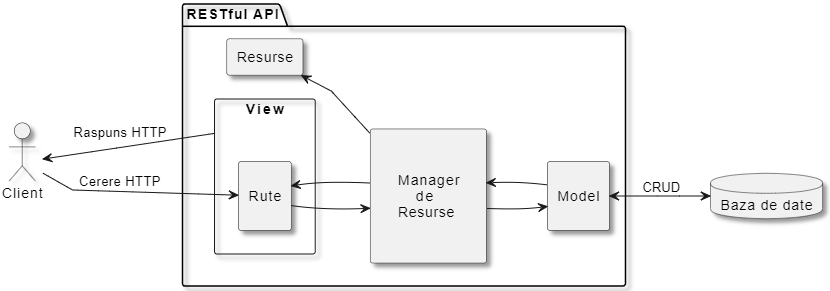
\includegraphics[scale=0.7]{figs/RESTfulStructure.png}
    \caption{Structura arhitecturii RESTful}
    \label{fig:RESTfulStructure}
\end{figure}

Principalul modul din arhitectura RESTful este modulul Resources, care semnifica resursa. O resursa reprezinta un set de date pe care un client il poate 
cere serverului prin transmiterea unui URL. Detalii despre URL se gasesc in capitolul \ref{sec:http}. Acesta reprezinta un identificator unic pentru 
fiecare resursa. Nu este necesar ca o resursa sa implementeze toate metodele HTTP, daca o metoda nu este implementata va fi returnat raspunsul de eroare 
405 semificand ca metoda nu este permisa. Exemplu de tranzactie intre client si server cu accentul pe resurse:
\begin{enumerate}
	\item clientul trimite un URL catre server
	\item serverul identifica resursa asociata URL-ului
	\item serverul interogheaza baza de date pentru resursa specificata
	\item serverul trimite un raspun care contine resursa ceruta si un status al tranzactiei
\end{enumerate}

Modulul Routes se ocupa de partea de rutare a cererilor primite de la client. Acest modul identifica pe baza adresei URL resursa de care clientul are nevoie, 
iar apoi informeaza modulul Resource Manager in legatura cu aceasta resursa.

Modulul Model se ocupa de operatiile cu baza de date, operatiile CRUD. Aceste operatii sunt creare, citire, modificare si stergere a unei intrari din 
baza de date. Rezultatul operatiei cu baza de date este returnat modulului Resource Manager.

Modulul Resource Manager este modulul central al acestei structuri si se ocupa cu extragerea resursei primita de la modulul Routes si a metodelor specifice 
acesteia, de exemplu, metodele HTTP GET si POST. Bazat pe aceste metode, modulul Resource Manager interogheaza baza de date. Raspunsul primit de la baza de date 
este validat si trimis catre modulul View.

Modulul View are sarcina de a formata datele primite de la modulul Resource Maganer in structura la care clientul se asteapta, apoi trimitand raspunsul catre 
client. 

Arhitectura RESTful API este asemanatoare cu modelul de design MVC, care semnifica Model View Controller si reprezinta o structurare a software-ului intern 
in trei module separate, Model si View care sunt identice cu modelele Model si View din RESTful API si Controller care inlocuieste modulul resource Manager 
din RESTful API.

Setul de reguli ce trebuie respectate pentru implementarea unei arhitecturi RESTful cuprind:
\begin{enumerate}
	\item Arhitectura aplicatiei trebuie sa fie de tipul client-server. Clientul trebuie separat de srever si de operatiile cu baza de date. Fiecare 
    participant al unei tranzactii trebuie sa fie independent de ceilalti.
	\item Lipsa starii inseamna ca o cerere trimisa de client trebuie sa contina toate informatiile necesare pentu ca aceasta sa fie onorata. Serverul 
	nu are voie sa retina informatii legate de client.
    \item Interfata uniforma specifica ca structura adreselor URL trebuie sa fie definita foarte clar, deoarece acestea reprezinta identificatorii unici 
    ai resurselor si implicit indentificarea corecta a resursei dorite.
    \item Clientul sau o alta componenta din retea poate sa retina raspunsurile de la server care sunt semnalate ca fiind memorabile cu scopul 
    optimizarii. 
    \item System pe nivele inseamna ca fiecare nivel este constient doar de nivelele din imediata apropiere a lui si ca intre server si client mai pot fi 
    adaugate nivele precum un server proxy.
\end{enumerate}

O metoda de versionare a software-ului unui server este prin adaugarea in adresa URL a unui numar care sa identifice unic o versiune, de exemplu, v1.1. 
Astfel se elimina problemele in care dupa o imbunatatire a software-ului, clientii care nu au aplicat modificarea nu mai pot accesa anumite resurse. 
Dezavantajul acestei metode este complexitatea software-ului din server care creste cu fiecare imbunatatire. Cu toate acestea, este considerata metoda 
cea mai avantajoasa.

\subsection{Flask framework}\label{sec:flask}
Framework-ul Flask este o biblioteca software de module reutilizabile care are scopul de a automatiza si standardiza modul in care sunt scrise aplicatiile 
web. Acesta este scris in limbajul de programare Python si este denumit micro-framework, deoarece are o complexitate redusa. Acesta contine doar module 
cu functionalitati de baza necesare in creearea unei aplicatii web, alte functionalitati care se doresc in aplicatie, cum ar fi utilizarea unei baze de 
date, fiind la latitudinea utilizatorului. In paragrafele urmatoare se vor detalia caracteristicile cheie ale ale framework-ului Flask.

Figura \ref{fig:FlaskProjectStructure} prezinta structura unui proiect Python utilizand framework-ul Flask.
\begin{figure}[H]
    \centering
    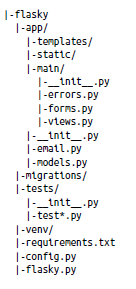
\includegraphics[scale=0.75]{figs/FlaskProjectStructure.png}
    \caption{Structura unui proiect Python utilizand Flask \cite{flaskweb}}
    \label{fig:FlaskProjectStructure}
\end{figure}

Structura de proiect prezentata in figura \ref{fig:FlaskProjectStructure} este detaliata in cele ce urmeaza:
\begin{enumerate}
	\item Fisierul flasky.py contine apelul prin care obiectul Flask este pornit, metoda run(). Aceasta metoda primeste ca parametrii adresa si 
    portul prin care serverul poate fi accesat. Este punctul principal, sau punctul de intrare in aplicatie si reprezinta o bucla infinita 
    in care sunt deservite cererile de la client.
	\item Fisierul requirements.txt contine numele bibliotecilor utilizate in proiect si versiunile acestora. Este un fisier foarte util atunci 
	cand o persoana preia proiectul pe o masina diferita si are nevoie sa creeze un mediu de lucru. Continutul acestui fisier poate fi usor generat 
    de comanda "pip freeze".
    \item Directorul venv/ contine toate bibliotecile instalate, cele continute in fisierul requirements.txt, si o referinta catre versiunea de python 
    utilizata. Astfel se creeaza un mediu de lucru separat fata de ceea ce este instalat global pe computer sau de alte proiecte. Acest director 
    trebuie creeat in faza de initiere a proiectului si atunci cand este preluat pe o alta masina de lucru.
    \item Directorul app contine fisierele aplicatiei, toate fisierele necesare ca aplicatia sa ruleze. Directoarele pentru testare si migrari sunt 
    separate.
    \item Fisierul view.py contine partea de rutare a cerintelor primite de la client catre resurse prin decoratori sau prin metode statice si 
    partea de formatare a raspunsului in structura asteptata de client. Acest fisier poate fi impartit in doua modula separate, routes.py si 
    view.py, fiecare avand o sarcina bine definita.
    \item Fisierul \_\_init\_\_.py din directorul app contine instantierea clasei Flask. Acest obiect se ocupa de toate cererile care vin de la client. 
    Pe langa instantiere mai poate contine metode de initializare a diferite module sau biblioteci pe care aplicatia le utilizeaza, cum ar fi conexiunea 
    la baza de date sau un sistem de versionare. Orice director care contine acest fisier este considerat un packet reutilizabil care poate fi inclus si 
    utilizat intr-o alta aplicatie. Atunci can directorul app este inclus in aplicatie, continutul fisierului \_\_init\_\_.py este prima portine de 
    cod care se ruleaza din acel pachet. 
\end{enumerate}

Decoratorii in python reprezinta o metoda prin care se seteaza o portiune de cod care sa fie executata atunci cand anumite evenimente au loc. De exemplu, 
la primirea unei cereri de la client decoratorul spune care portiune de cod, metoda, trebuie executata. In general aceasta metoda poarta denumirea de 
Handler. Decoratorii de tip route fac legatura intre adresa URL primita de la client si metodele resursei indentificata unic de adresa URL. Modul in  
care aceasta legatura este realizata de Flask, este prin creearea unei mapari a adreselor URL pe resurse.

Argumentele dinamice in adresa URL sunt adrese URL de baza care identifica o resursa, dar care au in plus un argument ce poate lua orice valoare. Acest 
argument este preluat de catre resursa si pe baza lui raspunsul care s-ar fi trimis in mod normal este personalizat generand un raspuns diferit.

Flask ofera un serviciu numit Request Hooks care ofera posibilitatea de a executa portiuni de cod inainte ca fiecare cerere de la client sa fie procesata, 
inainte doar de prima cerere de la client sau dupa ce cererea a fost procesata. Acest serviciu este util pentru cazurile in care se doreste realizarea 
conexiunii la baza de date sau autentificarea clientului de fiecare data cand o cerere este receptionata. Avantajul utilizarii acestui serviciu este 
cantitatea redusa de cod duplicat. Il loc sa se realizeze autentificarea in fiecare rutina specifica unei resurse, se realizeaza in mod generic inainte ca 
resursa sa fie accesata.

Cazurile de eroare, in Flask, pot fi personalizate. La primirea unei cereri de la client, daca aceasta este eronata, se poate transmite ca raspuns, pe langa 
codul de eroare, o pagina HTML sau un text care sa explice de ce a fost respinsa cererea.

Unele framework-uri din Python contin setul de instructiuni pentru integrara cu Flask, dar, dupa cum am prezentat si mai sus, Flask a fost creat pentru a fi 
integrat cu module externe, deci instructiunile necesare pentru integrarea cu acesta pot fi scrise de utilizator. Un exemplu de framework pentru baze de date 
care este integrat cu Flask este Flask-SQLAlchemy.

Micro-framework-ul Flask are un grad de flexibilitate foarte inalt comparat cu un full-framework. Flask a fost creat pentru a automatiza doar functionalitatile 
de baza necesare unei apicatii web, ceea ce inseamna ca nu are integrate componente pentru autentificare sau operatii pe baze de date, dar este 
compatibil cu componente externe. Acest lucru ofera posibilitatea de a utiliza framework-ul impreuna cu orice fel de baza de date sau orice tip de 
autentificare. Pe cealalta parte, un framework full, ca Django, ofera o gama de componente care pot fi utilizate pentru functionalitati precum 
operatiile pe baze de date si autentificare, deci utilizatorul este restrans in ceea ce priveste functionalitatile proiectului lui.

\subsection{Retrofit framework}\label{sec:retrofit}
Retrofit este o biblioteca scrisa in limbajul de programare Java care are scopul de a simplifica tranzactionarea cu un server RESTful. Intr-o arhitetura 
client-server aceasta biblioteca este implementata in partea clientului si este o interfata API care respecta constrangerile arhitecturii REST. Este o 
biblioteca utilizata cu preponderenta in aplicatiile pentru sistemul de operare Android. In urmatoarele paragrafe sunt descrise caracteristicile cheie 
ale acestei biblioteci.

Figura \ref{fig:RetrofitStructure} prezinta functionalitatea bibliotecii retrofit. Aceasta va fi detaliata in paragrafele urmatoare.
\begin{figure}[H]
    \centering
    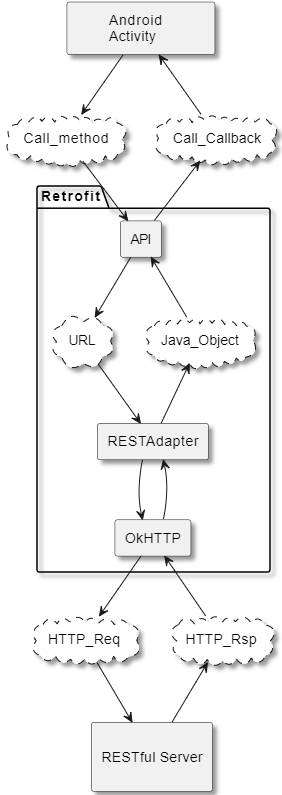
\includegraphics[scale=0.55]{figs/RetrofitStructure.png}
    \caption{Structura bibliotecii Retrofit}
    \label{fig:RetrofitStructure}
\end{figure}

Modulul Android Activity reprezinta interfata cu utilizatorul in sistemul de operare android. In urma unui eveniment, de exemplu, apasare buton sau 
o rutina periodica, se trimite o cerere catre modulul API, care la finalul tranzactiei va returna informatia care va fi afisata utilizatorului.

Modulul API contine mai multe modele si o interfata. In interfata sunt declarate metodele utilizate pentru a obine date de la server, de exemplu, metoda 
GetAllClients care va informa serverul sa puna in raspuns o lista cu toti clientii din baza de date. Utilizand adnotari aceste metode sunt mapate pe adrese URL. 
Metode returneaza un model, acesta fiind o clasa care contine toate campurile primite de la server in raspuns. De exemplu, campurile nume, adresa, 
varsta. La construirea obiectului Retrofit se realizeaza maparea dintre adresa URL, metode, si modele. API trimite catre modulul RESTAdapter un obiect 
al clasei Call. Acest obiect este initializat cu metoda care se doreste a fi executata utilizand obiectul Retrofit. Acesteia i se mai ataseaza 
doua rutine, una care este executata in cazul in care tranzactia a fost efectuata cu success si una care se executa in caz 
contrar.

Modulul RESTAdapter primeste de la modulul API obiectul de tip Call care contine toate informatiile necesare pentru a executa cererea catre server. Obiectul Call 
este transpus in format OkHTPP si trimis catre modulul OkHTTP. La finalul tranzactiei acesta primeste un raspuns de tipul OkHTTP pe care il mapeaza, 
pe baza informatiilor din obiectul retrofit, intr-un obiect al clasei model specifice. Acest obiect este returnat modulului API.

Modulul OkHTTP se ocupa de tranzactionarea efectiva prin retea. Primeste si returneaza obiecte specifice acestei biblioteci.

Aceasta biblioteca nu are implementat propriul mechanism petru tranzactionarea pachetelor HTTP, ci este integrata cu biblioteca OkHTTP. Aceasta din 
urma este o biblioteca complexa care implementeaza protocolul HTTP si toate mecanismele necesare de mitigare si rezolvare a erorilor in tranzactionarea 
prin retea. Are scopul de a automatiza complexitatea tranzactionarii prin retea pentru a usura utilizatorul de aceasta sarcina.

Biblioteca Retrofit este construita peste OkHTTP si rolul ei este de a automatiza parsarea si formatarea cererilor si raspunsurilor HTTP. Aceasta creeaza 
adresa URL si o trimite bibliotecii OkHTTP de unde este trimisa in retea. La primirea raspunsului, OkHTTP il trimite catre Retrofit care se ocupa de formatarea 
lui pentru a-l prezenta utilizatorului sub structura dorita, de exemplu, un obiect.

Fiecare metoda din Retrofit este identifica unic de o adresa URL si identifica unic un set de date cerut de la un server. Fiecare set de date este 
reprezentat printr-o clasa model. Acest lucru face posibila maparea dintre URL, metoda si model. Metodele sunt mapate la adrese URL prin adnotari. 
In aceste adnotari se specifica metoda HTTP si adresa URL. Cele mai utilizate adnotari sunt prezentate mai jos:
\begin{enumerate}
	\item @Path - aceasta adnotare permite utilizarea de campuri variabile in adresa URL. Aceasta adnotare este un parametru al functiei, iar valoarea 
	pe care o primeste la apelul metodei este pusa in adresa URL.
    \item @Body - aceasta adnotare permite inserarea in adresa URL a unei clase model. Aceasta adnotare se utilizeaza la metodele HTTP de salvare 
    in baza de date, cum ar fi metoda POST.
    \item @FormUrlEncoded - aceasta adnotare permite inserarea in adresa URL a unor campuri dintr-un model cu scopul de a-l modifica in baza de date.
\end{enumerate}

Metodele in Retrofit sunt doar declarate intr-o interfata, nu si implementate, iar instructiunile necesare pentru a converti o cerere HTTP intr-o clasa java 
sunt generate automat de catre acesta. Retrofit suporta conversia automata a multor tipuri de format a datelor, cum ar fi GSON sau SimpleXML, dar acopera si 
cazul in care serverul returneaza un format de date care nu este suportat, prin crearea unui convertor particular. Acest lucru presupune scrierea 
manuala a instructiunilor necesare convertirii raspunsului de la server in obiect Java. Acest lucru nu trebuie facut petru fiecare resursa in parte, ci 
in mod general, o singura data.

GSON este o biblioteca in Java care are rolul de a serializa un obiect Java intr-un format JSON, respectiv de a deserializa un obbiect in format JSON intr-un 
obiect java.   

Clasa Call suporta executarea cererii HTTP in mod sincron sau asincron. Este de preferat modul asincron, deoarece executia are loc pe un fir separat lasand 
firu de executie creator sa execute alte sarcini. Aceasta clasa este dedicata pentru fiecare tranzactie, o instanta a acesteia poate fi utilizata pentru 
o singura transmisie a unei cereri HTTP si receptie a unui raspuns HTTP. La finalul unei tranzactii obiectul este distrus.

\section{Baza de date MongoDB}\label{sec:mongodb}
MongoDB este o baza de date orientata pe documente fiind printre putinele baze de date diferita de cele uzuale care sunt relationale, adica stocheaza datele in tabele 
grupate intre ele prin relatii. Aceasta baza de date stocheaza datele in colectii de documente, de aici si denumirea de baza de date orientata pe documente. 
Structura acestui tip de baze de date permite un grad inalt de scalabilitate prin impartirea si distribuirea unei baze de date foarte mari pe mai multe 
servere. In paragrafele care urmeaza vor fi descrise caracteristicile cheie ale bazei de date.

Documentul reprezinta un singur set de date si poate fi asociat cu un inlocuitor al unui rand dintr-o baza de date relationala. Setul de date este stocat intr-un 
format numit BSON, Binary-JSON, care este o reprezentare in binar a formatului de fisiere JSON. Acesta din urma este un format de fisiere bazat pe text,
are o structura de tipul cheie-valoare si este usor de interpretat de catre om.

Figura \ref{fig:MongoDBDocument} prezinta structura unui document dintr-o baza de date MongoDB si, de asementea, formatul JSON.
\begin{figure}[H]
    \centering
    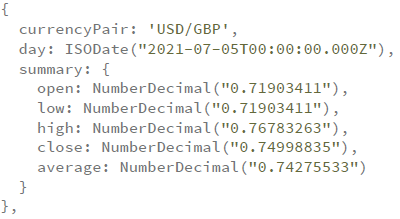
\includegraphics[scale=0.8]{figs/mongoDBDocument.png}
    \caption{Exemplu de document intr-o baza de date MongoDB \cite{mongoDB}}
    \label{fig:MongoDBDocument}
\end{figure}

Colectiile de tip serii in timp reprezinta un tip de colectii optimizate pentru a stoca si interoga documentele ordonate in timp. Aceste documente au in 
componenta un camp obligatoriu care reprezinta momentul de timp la care datele au fost achizitionate. In documentul prezentat in figura \ref{fig:MongoDBDocument} 
se poate observa perechea de valori "day" si data si ora in format ISO. Acest tip de colectii este utilizat cu preponderenta in IoT datorita faptului ca sunt 
optimizate pentru structura de date uzuala unui senzor. O astfel de structura contine, in general, un moment de timp la care achizitia de date a fost efectuata, 
un identificator unic al senzorului, in mod uzual adresa MAC, si valoarea metricii sau a metricilor achizitionate.

MongoDB creeaza automat un indice, o cheie primara, pentru fiecare document pentru a se asigura ca nu exista doua documente cu acelasi indice. In acelasi timp 
permite creearea unui indice secundar care poate contine unul sau mai multe campuri din setul de date si care are ca scop plierea pe structura fiecarui set de date 
si pe tipul de interogari cel mai des efectuate. In cazul seriilor in timp cele mai uzuale interogari sunt bazate pe timp, deci indicele ar trebui sa contina campul 
de timp la care trebuie specificata si ordonarea elementelor, de exemplu, intr-un sistem in care interogarea cea mai des intalnita este retragerea documentelor 
din ultimele 24 de ore ordonarea trebuie efectuata in ordine descrescatoare a timpului. Pe langa campul de timp, indicele mai poate contine inca un camp pentru 
a acoperi cazurile in care interogarea se face nu doar pe o perioada de timp, ci si pe o alta valoare continuta in setul de date, de exemplu, campul care contine 
adresa MAC a senzorului. MongoDB va stoca datele in functie de acest indice obtinand astfel interogari foarte eficiente. Totodata un indice prea complex sau 
scris incorect va creste complexitatea scrierii in baza de date si automat va scadea eficienta.

\section{Componente Hardware}\label{sec:af_hw_components}
\subsection{Platforma de dezvoltare Arty Z7}\label{subsec:af_artyz7}
Arty Z7 este o platforma de dezvoltare creata de compania Digilent care are ca nucleu sistemul integrat Zynq-7000 de la Xilinx si o multitudine de porturi si 
componente periferice pentru adaptarea la diferite proiecte embedded. Arhitectura interna a sistemului integrat Zynq-7000 este formata dintr-un procesor de tip 
ARM Cortex-A9 cu doua nuclee si partea logica FPGA 7-series. Aceasta combinatie ofera capabilitatea de a paraleliza executia unui software prin mutarea anumitor 
rutine intensive, cum ar fi procesarea de semnale, din acesta in partea logica a sistemului integrat oferind un nivel de performanta mai inalt.

Platforma de dezvoltare Arty Z7 ofera ca sursa de ceas un crystal cu frecventa de 50 MHz care este conectat ca intrare in procesorul ARM Cortex-A9. Procesorul 
multiplica semnalul de ceas printr-un circuit PLL, iar apoi il distribuie componentelor periferice.

Pentru crearea unui design hardware, compania AMD Xilinx pune la dispozitie mediul de dezvoltare Vivado Design Suite. Acesta contine toate uneltele necesare pentru 
crearea unui design hardware de la zero, unelte precum blocuri IP uzuale care pot fi adaugate direct intr-o schema de desing, sintetizarea si analiza schemei de 
design si depanarea problemelor. De asemenea, acest mediu de programare ofera posibilitatea de utilizare a sistemului integrat Zynq-7000 ca pe un microcontroller. 
Acest lucru este realizat automat de catre mediul de dezvoltare Vivado prin adaugarea in design a blocului IP "Zynq7 Processing System". Prin accesarea acestui block 
este deschisa o interfata din care se pot alege sursa si frecventa semnalului de ceas, perifericele care se doresc a fi utilizate (I2C, SPI, GPIO), intreruperi etc.

Design-ul placii de dezvoltare Arty Z7 leaga o parte din perifericele de pe placa la partea logica a sistemului integrat Zynq-7000 si o parte la partea de procesare. 
De exemplu, conectorii MicroUSB, USB, Ethernet sunt conectati la partea de procesare a sistemului integrat, iar porturile Pmod, butoanele si o parte din GPIO-uri sunt 
legate la partea logica.

Pentru dezvoltarea codului sursa al unei aplicatii, compania Xilinx pune la dispozitie mediul de dezvoltare Xilinx SDK care este bazat pe platforma Eclipse. Pentru 
integrarea codului sursa cu design-ul hardware acesta pune la dispozitie un mecanism automat care pe baza unui fisier ".hdf" generat de Vivado creeaza o biblioteca sub 
forma unui proiect nou.

Mediul de dezvoltare Vitis oferit de compania AMD Xilinx este mai nou si a fost creeat special pentru sistemele integrate care includ FPGA si procesor ARM. Acesta combina 
mediul de dezvoltare Vivado Design Suite cu mediul de dezvoltare Xilinx SDK intr-un singur mediu de dezvoltare care ofera un nivel mai inalt de abstractizare.

\subsection{Controlerul de retea ATWINC1500}\label{subsec:af_atwinc}
ATWINC1500 este un sistem integrat intr-un singur cip care a fost creat pentru a simplifica procesul de adaugare a unei conexiuni wireless la o aplicatie embedded. 
Acesta contine stiva de comunicare TCP/IP integrata in cip, ceea ce elibereaza microcontroller-ul gazda de gestionarea retelei si reduce timpul necesar pentru integrarea 
acestuia intr-un poriect. Suporta standardele de comunicatie Wi-Fi IEEE 802.11 b/g/n si opereaza in banda de frecventa 2.4 GHz.

WINC1500-XPRO reprezinta placa de extensie pentru modulul ATWINC1500 care ofera un conector de 20 de pini pentru a facilita integrarea acestuia cu un microcontroler 
gazda. Prin acest conector se realizeaza alimentarea intregii placi de extensie si legarea acesteia la interfata de comunicare SPI si la pinii de control.

Interfata API care defineste setul de reguli si tipul de mesaje acceptate de modulul ATWINC1500 este implementata in driverul oferit de compania Microchip. Aceasta 
implementare trebuie adaptata la platforma utilizata, iar pentru acest lucru in fisierul antet "winc1500\_api.h" exista declaratii ale rutinelor care sunt specifice 
fiecarei platforme si care trebuie implementate de catre integratorul driverului. Acestea sunt numite functii stub si implementarea corecta a acestora este necesara 
pentru functionarea rutinelor driverului:
\begin{enumerate}
	\item m2mStub\_PinSet\_CE - implementeaza managementul pinului CHIP\_EN. Valoarea 1 logic activeaza modulul ATWINC1500, iar valoarea 0 logic il dezactiveaza.
	\item m2mStub\_PinSet\_RESET - implementeaza managementul pinului RESET. Acesta este utilizat pentru resetarea modulului si este activ in 0 logic.
	\item m2mStub\_PinSet\_SPI\_SS - implementeaza managementul pinului SS al interfetei SPI. 
	\item m2mStub\_EintEnable - activeaza intreruperile pe pinul IRQN al modulului.
	\item m2mStub\_EintDisable - dezactiveaza intreruperile pe pinul IRQN al modulului.
	\item m2mStub\_SpiTxRx - implementeaza functionalitatea de transfer de date prin interfata SPI.
	\item m2mStub\_GetOneMsTimer - accesseaza registrul Counter al timerului dedicat pentru modulul ATWINC1500 si returneaza valoarea acestuia.
\end{enumerate}

\

Principalele functionalitati ale acestui controller de retea sunt prezentate in urmatoarele puncte din perspectiva rutinelor oferite de driver:
\begin{itemize}
	\item m2m\_wifi\_connect - implementeaza conectarea la un router. Primeste ca parametrii numele retelei, tipul de securitate utilizat de catre retea si parola acesteia.
	\item m2m\_wifi\_p2p - implementeaza conectarea punct la punct cu un alt dispozitiv utilizand protocolul Wi-Fi Direct. In fisa de date a modulului ATWINC1500 
    \cite{atwinc1500} este precizat ca versiunile de microprogram de pe modulul ATWINC1500 mai noi de versiunea din data de 10/2018 nu mai suporta acest protocol.
    \item m2m\_enable\_ap - aceasta functie pune modulul ATWINC1500 in modul AP, in care acesta se comporta ca un punct de access care suporta o singura conexiune.
    \item socket, connect, bind, listen, recv, send - aceste functii sunt utilizate pentru crearea si gestionarea conexiunilor prin intermediul unui Socket. 
    Functia "connect" este utilizata pentru conectarea la un Socket, iar functiile "bind" si "listen" sunt utilizate pentru asteptarea unei conexiuni din exterior. Prima 
    functionalitate este specifica unui dispozitiv cu rol de Client, iar cea de-a doua este specifica unui dispozitiv cu rol de Server.
\end{itemize}

\subsection{Senzorul HDC1080}\label{subsec:af_hdc1080}
Acesta este un senzor digital creeat de compania Texas Instruments care masoara temperatura si umiditatea mediului in care se afla cu un consum de energie foarte mic. 
Pentru masurarea umiditatii acesta utilieaza un senzor capacitiv a carei variatie a capacitantei este transformata intr-un semnal digital, iar pentru masurarea 
temperaturii acesta utilizeaza un material semiconductor ale carei variatii in tensiune sunt transformate in semnal digital.

PmodHYGRO reprezinta platforma, placa de circuite integrate, pe care se afla senzorul HDC1080. Aceasta ofera circuitele pasive necesare functionarii senzorului si 
un conector pmod care face usoara conectarea acestuia la o platforma gazda.

Protocolul de comunicare al senzorului este I2C. Acesta are rolul de slave, iar microprocesorul gazda are rolul de master pe magistrala I2C. Modulul HDC1080 are un 
registru indicator care mentine ultima adresa de la care s-a efectuat o citire sau o scriere. Pentru realizarea unei scrieri sau citiri a unui registru, mai intai 
trebuie scris registrul indicator, iar apoi efectuata scrierea sau citirea efectiva a registrului dorit. Primul octet transmis contine adresa I2C pe 7 biti a 
modulului HDC1080 si bitul care indica o scriere sau o citire. Al doilea octet contine adresa registrului cu care se efectueaza operatia de citire sau scriere. 
In cazul unei scrieri, dispozitivul master transmite al doile si al treilea octet care contin date fara a intrerupe comunicatia. In cazul unei citiri, dupa scrierea 
registrului indicator se initiaza tranzactia I2C de citire in care se transmite din nou adresa I2C si bitul de citire, iar apoi se receptioneaza un numar de octeti. 
Registrul indicator al senzorului se incrementeaza automat dupa citirea unei adrese, ceea ce face posibila citirea temperaturii si umiditatii, care sunt doi registri 
diferiti, intr-o singura tranzactie I2C de citire.

Figura \ref{fig:PI_HDC1080ReadOperation} prezinta o captura a unei tranzactii I2C pentru citirea metricilor senzorului efectuata cu un analizor logic. Figura contine 
inceputul tranzactiei in partea de sus si finalul tranzactiei in partea de jos, mijlocul tranzactiei fiind omis deoarece este format din incercari de initiere a unei 
tranzactii la care senzorul raspunde cu NACK. In paragraful urmator figurii este descrisa in detaliu tranzactia.
\begin{figure}[H]
    \centering
    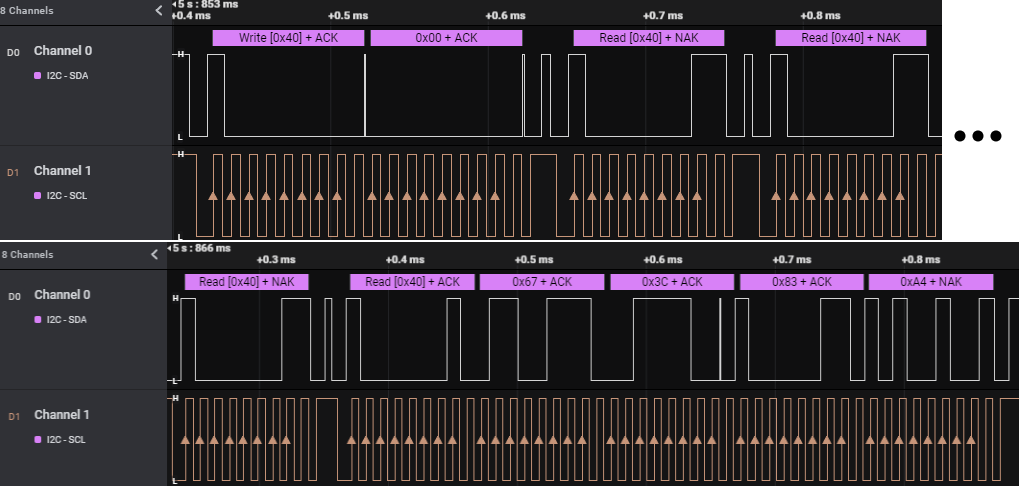
\includegraphics[scale=0.40]{figs/PI_HDC1080ReadOperation.png}
    \caption{Operatia de citire a temperaturii si a umiditatii}
    \label{fig:PI_HDC1080ReadOperation}
\end{figure}

Pentru a incepe o achizitie de temperatura si umiditate trebuie executata o operatie de scriere a registrului pointer in care adresa scrisa in registrul pointer este 
0x00, adica adresa registrului de temperatura. Acest lucru este reprezentat de primii 2 octeti din partea de sus a figurii la care senzorul raspunde cu ACK. Al treilea 
si al patrulea octet din partea de sus a figurii reprezinta initieri a unei tranzactii de citire la care senzorul raspunde cu NACK, deoarece continutul acestuia nu a 
fost actualizat. Primul octet din partea de jos a figurii reprezinta tot o initiere a operatiei de citire la care senzorul raspunde cu NACK. La al doilea octet, in schimb, 
senzorul raspunde cu ACK, ceea ce inseamna ca achizitia s-a incheiat si valorile temperaturii si a umiditatii pot fi citite. Octetii 3 si 4 reprezinta valoarea 
temperaturii, iar octetii 5 si 6 reprezinta valoarea umiditatii. Ambele valori sunt reprezentate pe 16 biti avand cel mai putin semnificativi 2 biti mereu 0x00, 
deoarece rezolutia convertorului din analog in digital este de maximum 14 biti. Pentru a obtine temperatura in grade celsius si umiditatea in procent, valorile 
obtinute la finalul achizitiei trebuie trecute prin doua formule, una specifica temperaturii si una specifica umiditatii. Aceste formule sunt oferite de catre 
fisa de date a senzorului \cite{hdc1080}.

\subsection{Senzorul SGP40}\label{subsec:af_sgp40}
SGP40 \cite{sgp40} este un senzor digital creat de compania Sensirion care masoara concentratia compusilor organici volatili (VOC) din aer. Tehnologia de masurare este compusa 
dintr-un element care incalzeste un strat semiconductor cu oxid metalic care cauzeaza o reactie chimica atunci cand compusii organici volatili sunt prezenti in aer. 
Aceasta reactie produce schimbari in rezistivitatea semiconductorului care este transformata in semnal digital.

Interfata de comunicare dintre senzor si un microcontroller gazda este I2C, senzorul avand rolul de slave, iar microcontroller-ul rolul de master.

Senzorul SGP40 include algoritmi pentru compensarea temperaturii si a umiditatii, asigurand astfel acuratetea si stabilitatea datelor in diferite conditii.

Compusii organici volatili (VOC) reprezinta poluatori uzuali ai aerului si sunt emisi de produse precum vopsele, materiale de constructii sau produse de curatenie.

Pentru integrarea acestui senzor cu un microcontroller gazda Sensirion ofera un driver sub licenta deschisa. Acesta contine rutinele necesare utilizarii senzorului 
intr-o aplicatie.

Sensirion ofera un algoritm pentru interpretarea datelor citite de la senzorul SGP40 sub licenta libera. Acest algoritm primeste ca intrare valorile brute citite de 
senzor in unitatea de masura micrometru sau parti pe milion si returneaza un indince al compusilor organici volatili. Sensirion ofera un cod de culori care corespunde 
cu valorile indicelui returnat de algoritm pentru interpretarea acestuia din punct de vedere al calitatii aerului. Algoritmul compenseaza variatia valorilor care exista 
intre senzorii SGP40, iar semnalul brut de intrare trebuie oferit la un interval constant de o secunda.

\subsection{Senzorul SPS30}\label{subsec:af_sps30}
SPS30 \cite{sps30} este un senzor digital creat de compania Sensirion care masoara concentratia particulelor in suspensie (PM) din aer. Tehnologia de masurare este numita 
"Laser Scattering" si presupune o sursa de lumina laser care lumineaza particulele care trec printr-o camera de detectie si un fotodetector care detecteaza 
dispersia luminii cauzata de aceste particule. Intensitatea cu care este dispersata lumina ofera informatii legate de marimea si concentratia particulelor care 
este transformata in semnal digital.

Particulele in suspensie reprezinta poluatori uzuali ai aerului care sunt generati de praf, polen, fum etc. Senzorul are capacitatea de a masura 4 dimensiuni ale 
acestor particule:
\begin{itemize}
	\item PM1.0 - particule in suspensie cu un diamentru de 1.0 micrometri sau mai mic.
	\item PM2.5 - particule in suspensie cu un diamentru de 2.5 micrometri sau mai mic.
	\item PM4.0 - particule in suspensie cu un diamentru de 4.0 micrometri sau mai mic.
	\item PM10.0 - particule in suspensie cu un diamentru de 10.0 micrometri sau mai mic.
\end{itemize}

Senzorul este incapsulat intr-o unitate metalica pentru a diminua contaminarea componentelor optice cu praf sau alte particule. Unitatea metalica contine pe o latura 
fante pentru accesul aerului. Pentru a controla fluxul aerului care intra in senzor, acesta contine in spatele fantelor un ventilator care functioneaza atunci cand este 
realizata o masuratoare sau in procesul de curatare automata.

SPS30 suporta doua interfete de comunicare pentru integrarea cu un microcontroler gazda, UART sau I2C. Acesta contine un conector de tip mama cu 5 pini pentru realizarea 
conexiunii cu un modul extern. 2 dintre acesti pini sunt utilizati pentru alimentarea cu 5V a senzorului, unul dintre pini are rolul de selectare a interfetei de comunicare, 
iar cei 2 pini ramasi pot fi utilizati ca SDA si SCL sau ca RXD si TXD pentru comunicarea utilizand protocolul I2C respectiv UART.

Sensirion ofera un driver sub licenta deschisa pentru interfatarea cu acest senzor care contine rutinele necesare controlului senzorului.

 % \chapter{Analiză și Fundamentare Teoretică}

\chapter{Proiectare de detaliu și implementare}
\pagestyle{fancy}

Acest capitol prezinta in detaliu solutia propusa pentru un sistem de monitorizare a temperaturii si a umiditatii. Aceasta include protocoalele de 
comunicatie utilizate, limbajele de programare si arhitecturi de abstractizare.

Arhitectura generala a sistemului este compusa din 5 componente pricipale interconectate pentru a crea o retea bine definita si cu o flexibilitate
ridicata:
\begin{enumerate}
	\item Aplicatie Android
	\item MQTT Broker
	\item Server
	\item Baza de date
	\item Senzor
\end{enumerate}

\

Figura \ref{fig:ArhitecturaGenerala} prezinta arhitectura generala a sistemului continand modulele principale ale acestuia si protocoalele de comunicatie 
dintre acestea.
\begin{figure}[H]
    \centering
    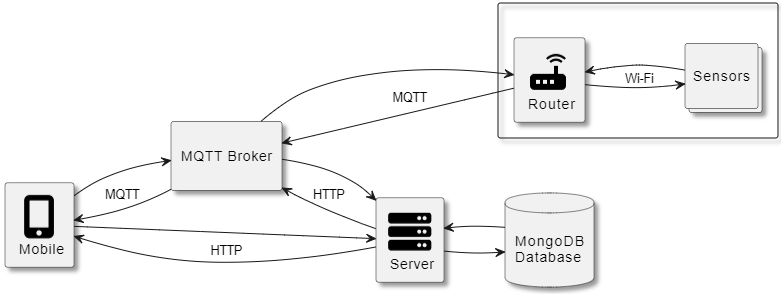
\includegraphics[scale=0.72]{figs/ArhitecturaGenerala.png}
    \caption{Arhitectura generala a proiectului}
    \label{fig:ArhitecturaGenerala}
\end{figure}

In subcapitolele urmatoare va fi descris in mod detaliat fiecare modul al sistemului si protocoalele de comunicatie utilizate pentru comunicarea dintre 
acestea.

\section{Aplicatia Android}\label{sec:pi_appandroid}
Aplicatia Android reprezinta interfata cu utilizatorul oferindui acestuia un mod usor de a gestiona mai multi senzori si de a monitoriza datele venite de la
acestia. Este scrisa in limbajul de programare Java si ruleaza pe sistemul de operare Android. Proiectul este scris in mediul de dezvoltare integrat Android 
Studio IDE.

In sistemul de operare Android clasele care definesc o interfata grafica sunt denumite activitati. La deschiderea aplicatiei este deschis firul de executie principal 
care are sarcina de a afisa interfetele grafice si de a gestiona actiunile utilizatorului, de exemplu, apasare de buton. Fiecare clasa de tip activitate extinde 
clasa AppCompatActivity care ofera componente pentru afisarea grafica si metode callback pentru gestionarea navigarii intre mai multe activitati. 

Aplicatia este compusa din 2 activitati principale si cateva secundare:
\begin{enumerate}
	\item ActivityWelcome - reprezinta activitatea care este afisata la deschiderea aplicatiei.
	\item ActivitySensor - reprezinta activitatea care este afisata atunci cand utilizatorul selecteaza un senzor din lista.
	\item ActivityInstall - reprezinta un grup de activitati secundare afisate atunci cand utilizatorul instaleaza un senzor nou. Fiecare dintre aceste 
	activitati reprezinta un pas din procesul de instalare.
\end{enumerate}

\

Figura \ref{fig:AndroidClassDiagram} prezinta diagrama de clase a aplicatiei Android.
\begin{figure}[H]
    \centering
    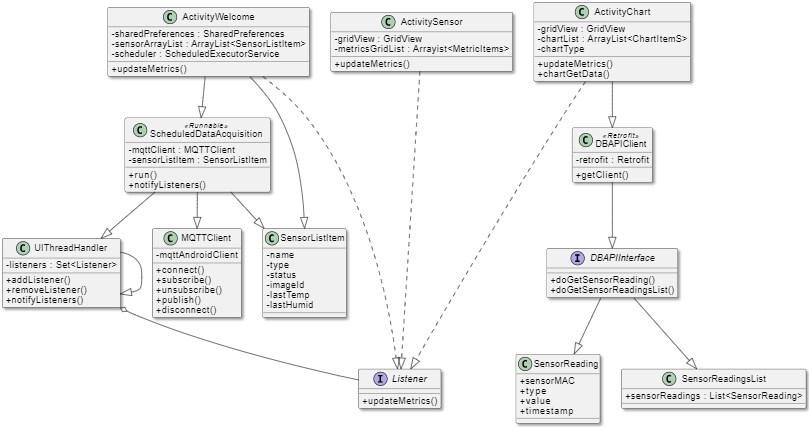
\includegraphics[scale=0.64]{figs/AndroidClassDiagram.png}
    \caption{Arhitectura generala a proiectului}
    \label{fig:AndroidClassDiagram}
\end{figure}

La incarcarea primei activitati care este afisata pe ecranul dispozitivului mobil, numita ActivityWelcome, se extrage din memorie o lista de senzori care au fost 
instalati in prealabil. Daca nu exista senzori instalati, aceasta lista nu va contine elemente. Lista este parcursa si pentru fiecare senzor este pornit un nou 
fir de executie periodic. Acest fir de executie are rolul de a gestiona conexiunea cu modulul MQTT Broker pentru senzorul respectiv, iar periodicitatea 
acestuia perimite verificarea si reincercarea conexiunii la un interval fix de timp. Apoi aceasta lista este afisata in interfata grafica. Fiecare element din lista 
contine: denumirea senzorului, tipul de senzor, statusul conexiunii si o imagine reprezentativa a senzorului.

Pentru memorarea senzorilor installati este utilizata biblioteca SharedPreferences. Aceasta contine rutine pentru salvarea datelor intr-un fisier din memoria 
dispozitivului mobil intr-un format de forma (cheie, valoare). Primul camp din acest fisier reprezinta numarul de senzori salvati, iar campurile ce urmeaza 
reprezinta senzorii instalati. Aceasta biblioteca este potrivita pentru memorarea datelor sub forma (cheie, valoare) si pentru compatibilitatea cu versiuni mai 
vechi de Android, spre deosebire de alte biblioteci precum DataStore care sunt potrivite pe seturi de date complexe si functioneaza doar in versiunile mai noi de 
Android.

Pentru firele de executie periodice este utilizata biblioteca ScheduledThreadPoolExecutor. Acesasta permite crearea unui grup de fire de executie care se executa
in paralel, spre deosebire de biblioteca Timer care are un singur fir de executie, iar o sarcina de durata mai lunga poate intarzia alte sarcini care asteapta 
executia. De asemenea, in cazul unei erori, doar sarcina in care a aparut eroarea va fi oprita, celelalte sarcini fiind executate in mod obisnuit. Aceasta 
biblioteca ofera siguranta continuarii executiei aplicatiei in cazul unei erori izolate.

La selectarea de catre utilizator a unui senzor din lista afisata este deschisa o noua activitate, numita ActivitySensor, iar la atingerea butonului de adaugare a unui 
nou senzor este deschisa prima activitate din grupul de activitati specifice instalarii. Pentru navigarea la o noua activitate si pentru transferarea de informatii intre 
activitati este utilizata clasa Intent. Aceasta clasa reprezinta o descriere abstracta a unei operatii. Cea mai semnificativa utilizare a acesteia este pentru operatia de 
deschidere a unei noi activitati. Pentru aceasta operatie se apeleaza functia startActivity() care primeste ca parametru o instanta a clasei Intent care contine informatiile 
necesare pentru ca operatia sa fie executata. Informatii precum activitatea parinte si activitatea care urmeaza a fi executata sunt necesare, iar in plus pot fi adaugate 
informatii care sa fie transferate catre activitatea copil utilizant functia putExtra() care primeste ca parametru o structura de tipul (cheie, valoare).

Pentru fiecare fir de executie specific unui senzor se creaza o instanta a clasei ScheduledDataAcquisition care implementeaza interfata runnable si executa periodic o rutina 
in care se verifica daca senzorul este conectat la modulul MQTT Broker. La prima executie senzorul este considerat deconectat si se executa rutina de conectare. 
Aceasta rutina utilizeaza clasa MQTTClient care ofera metodele necesare realizarii si gestionarii conexiunii cu modulul MQTT Broker. Pentru realizarea conexiunii se 
executa metoda connect a clasei MQTTClient care primeste ca paramterii 2 rutine callback. Aceste rutine definesc actiuni ce sunt executate atunci cand au loc 
diferite evenimente in tranzactionarea cu modulul MQTT Broker. Mai jos sunt enumerate cele mai importante astfel de evenimente:
\begin{itemize}
	\item Connectarea cu success la modulul MQTT Broker - cand are loc acest eveniment se executa rutina de subscriere pentru receptionarea in timp real a datelor de la 
	senzor.
	\item Pierderea conexiunii - acest eveniment va modifica statusul conexiunii din lista de senzori a-i activitatii ActivityWelcome si din ActivitySensor.
	\item Receptia unui mesaj - acest eveniment va apela metoda notifyListeners() a obiectului UIThreadHandler care va actualiza ultima valoare de temperatura si 
	umiditate afisata in activitatile ActivityWelcome si ActivitySensor. De asemenea, acest eveniment va verifica si statusul conexiunii senzorului si il va schimba 
	daca este cazul.
\end{itemize}

Clasa MQTTClient utilizeaza o instanta a clasei MqttAndroidClient oferita de biblioteca eclipse.paho.mqttv3 care reprezinta o implementare asincrona a 
al unui client al protocolului MQTT si are rolul de a gestiona impachetarea messajelor in formatul protocolului MQTT si tranzactionarea acestora cu un server MQTT. De asemenea, 
clasa MQTTClient defineste rutine de gestionare a exceptilor ridicate de obiectul MqttAndroidClient in cazul unei erori. 

Clasa UIThreadHandler are rolul de a efectua modificari in interfetele grafice de pe un fir de executie extern. Clasele de tip activitate sunt executate pe un fir de executie 
care are rolul strict de a raspunde la actiunile utilizatorului si doar acest fir de executie poate face modificari in interfata grafica, iar interogarea bazei de date sau 
receptionarea de date de la modulul MQTT sunt executate pe fire de executie diferite. Aceasta clasa realizeaza transferul de date sau evenimente care necesita modificarea 
interfetei grafice si care au fost primite pe un fir de executie extern catre firul de executie al interfetei grafice. Pentru a realiza acest transfer, instanta clasei  
UIThreadHandler mentine o lista de clase de tip Listener. Activitatile AvtivityWelcome si ActivitySensor sunt clase de tip Listener, deoarece implementeaza interfata 
Listener si metoda updateMetrics() a acesteia, iar la creare se inregistreaza in lista de obiecte Listener mentinuta de instanta UIThreadHandler. Fiecare activitate 
defineste in metoda updateMetrics() ce anume va fi modificat in interfata grafica. Atunci cand sunt receptionate date de la modulul MQTT Broker, se executa metoda 
notifyListeners() a obiectului UIThreadHander. Aceasta metoda parcurge lista de clase de tip Listener si pentru fiecare apeleaza metoda updateMetrics(). Aceasta metoda nu este 
apelata direct, ci prin obiectul Handler care primeste ca parametru o rutina de tip Runnable si care este pus intr-o coada de executie a interfetei grafice.

La selectarea unui element din lista de senzori afisata in activitatea ActivityWelcome este creata activitatea ActivitySensor. Rolul acesteia este de a prezenta informatiile 
senzorului selectat si datele de temperatura si umiditate ale acestuia sub forma grafica si sub forma a 2 campuri care contin doar ultima valoare receptionata. La creare 
se citeste din obiectul Intent primit de la activitatea ActivityWelcome informatiile senzorului intr-un obiect SensorListItem, se afiseaza informatiile senzorului in 
interfata grafica, se initializeaza graficele de temperatura si umiditate si se interogheaza baza de date pentru valorile din ultimele 10 minute. La primirea valorilor 
citite din baza de date, acestea sunt scrise in graficul de temperatura, respectiv umiditate. Daca nu exista date in ultimele 10 minute inseamna ca senzorul nu este conectat, iar 
statusul acestuia este modificat corespunzator. 

Pentru interogarea bazei de date este utilizata biblioteca Retrofit a carei functionalitate teoretica este descrisa in sectiunea \ref{sec:retrofit}. Pentru implementarea 
rutinelor de interogare a bazei de date utilizand aceasta biblioteca sunt utilizate urmatoarele clase din figura \ref{fig:AndroidClassDiagram}:
\begin{itemize}
	\item Clasa DBAPIClient - are rolul de a crea un obiect de tip Retrofit. Pentru crearea acestuia sunt necesare: adresa URL a server-ului, un obiect GsonConverterFactory 
	pentru convertirea automata a datelor si o instanta a clasei OkHttpClient.
	\item Interfata DBAPIInterface - declara metodele pentru interogarea bazei de date utilizand adnotari.
	\item Clasa SensorReading - este o clasa model care contine campurile receptionate in raspunsul metodei doGetSensorReading().
	\item Clasa SensorReadingsList - este o clasa model care contine o lista de obiecte de tip SensorReading. Aceasta lista reprezinta raspunsul metodei doGetSensorReadingsList().
\end{itemize}

La initierea unei interogari a bazei de date se obtine obiectul Retrofit utilizand metoda getClient() a clasei DBAPIClient. Se apeleaza metoda create() a obiectului Retrofit care 
primeste ca parametru interfata DBAPIInterface, iar pe baza acestei interfete, Retrofit va genera automat o clasa care contine implementarea metodelor declarate in aceasta. 
Utilizand instanta clasei creata automat se acceseaza una din metodele acesteia si se pune intr-o coada de transmisie impreuna cu o metoda callback care va fi executata cand 
este receptionat raspunsul de la server sau cand expira timpul de asteptare. La receptionarea raspunsului, biblioteca Retrofit va interpreta datele receptionate in format GSON 
bazat pe clasa model specifica metodei care s-a executat si va crea un obiect de acest tip. In metoda callback se citeste obiectul si se adauga valorile de temperatura si 
umiditate in graficul respectiv fiecareia. Pentru interpretare, a fost utilizat obiectul GsonConverterFactory care a fost instantiat la crearea obiectului Retrofit.

Pentru instalarea unui nou senzor, la apasarea butonului de adaugare din activitatea ActivityWelcome se deschide prima activitate din setul de activitati pentru instalare. 
Aceasta activitate cere utilizatorului inserarea datelor de conectare la senzor oferite in manualul de instalare. La apasarea butonului Next se deschide a activitatea de 
instalare specifica pasului doi in care se cere introducerea informatiilor router-ului prin care i se ofera senzorului access la internet. Al treila pas este reprezentat 
printr-o activitate care afiseaza durata si progresul procesului de instalare. La acest pas se realizeaza conexiunea completa a senzorului. La finalizeara conexiunii apare 
in activitate un buton care va redeschide activitatea ActivityWelcome, iar noul senzor adaugat va fi afisat in lista acesteia. 

\section{MQTT Broker}\label{sec:pi_mqttbroker}
Aici nu am diagrama.
Am folosit mosquito.
Mosquito ruleaza intr-o masina virtuala din google.
Configurarea si startarea mosquito.
Utilizarea fisierului care executa task-uri automat in linux.
Configurarea IP-ului pe care mosquito asculta.
Ce topic-uri exista. Formatul topic-urilor.

\section{RESTful Server}\label{sec:pi_restserver}
Scris in python.
Diagrama care prezinta subscriber-ul for all.
Am utilizat Flask detaliere functionalitate Flask.
Diagrama care prezinta RESTful API.
Problema cu timpul din python.

\section{Baza de date}\label{sec:pi_bazadedate}
Formatul datelor.
Avantaje ale time database si a indicilor de cautare.
Prezentare operatie de agregare. Aici sau la Restful server?

\section{Senzor}\label{sec:pi_senzor}


{\color{blue}Împreună cu capitolul \textbf{precedent} și cel \textbf{următor} trebuie să reprezinte aproximativ 70\% din total.\\}

Scopul acestui capitol este de a documenta aplicația dezvoltată în așa fel încât dezvoltarea și întreținerea ulterioară să fie posibile.
Cititorul trebuie să identifice funcțiile principale ale aplicației din ceea ce este scris aici.
Capitolul ar trebui sa conțină (nu se rezumă neapărat la):
\begin{itemize}
	\item schema generală a aplicației
	\item descrierea fiecărei componente implementate, la nivel de modul
	\item diagrame de clase, clase importante și metode ale claselor importante.
    \item diagrame de baze de date
\end{itemize}
 % \chapter{Proiectare de Detaliu și Implementare}

\chapter{Testare și validare}
\pagestyle{fancy}

In acest capitol sunt descrise testele efectuate asupra sistemului de monitorizare a calitatii aerului si rezultatele obtinute in urma acestora. In cadrul fiecarui 
test vor fi prezentate capturi de ecran ale aplicatiei Android continand valorile raportate de senzor si grafice. In capturile de ecran se va observa ca fiecare 
valoare prezentata are o culoare care se modifica pe parcursul testului. Aceasta culoare reprezinta gradul de calitate al aerului:
\begin{itemize}
	\item Verde - Calitatea aerului este foarte buna.
	\item Galben - Calitatea aerului este moderata.
	\item Portocaliu - Calitatea aerului este slaba. 
	\item Rosu - Calitatea aerului este foarte slaba.
	\item Mov - Calitatea aerului este periculoasa.
	\item Maro - Calitatea aerului este extrem de periculoasa.
\end{itemize}

\section{Testare raspuns senzori la schimbarile mediului}\label{sec:tv_environmental_variation}
\subsection{Variatia temperaturii}\label{subsec:tv_temperature_variation}
In acest test temperatura a fost variata de la cea a camerei pana la 55 de grade celsius utilizand o camera termica. S-a ales limita de 55 de grade celsius deoarece 
senzorul de particule in suspensie SPS30 are specificata in fisa de date ca temperatura de functionare maxima 60 de grade celsius.

Pentru compararea valorilor raportate de senzorul HDC1080 a fost utilizat senzorul de temperatura al camerei termice. Acest senzor utilizeaza 3 termocuple de tip T 
pentru raportarea la fiecare minut a temperaturii din camera termica. Valorile raportate sunt reprezentate grafic.

In prima captura de ecran din figura \ref{fig:tv_temp_var_sensor_view}, starea initiala, se observa ca toate valorile prezinta o calitate a aerului buna, exceptand umiditatea care prezinta o calitate a aerului 
moderata. 

In a doua captura de ecran din figura \ref{fig:tv_temp_var_sensor_view}, starea intermediara, se observa cresterea temperaturii la 38.193 grade celsius care prezinta o calitate a aerului periculoasa si scaderea umiditatii 
la 37.615 \% care prezinta o calitate a aerului moderata. Indicii particulelor in suspensie (PM1.0, PM2.5, PM4.0 si PM10.0) si Indicele Compusilor Organici Volatili 
nu au suferit modificari notabile prezentand in continuare o calitate a aerului buna.

In a treia captura de ecran din figura \ref{fig:tv_temp_var_sensor_view}, momentul opririi incalzitorului camerei termice, se observa ca valoarea temperaturii a crescut la 54.115 grade celsius reprezentand un mediu foarte 
periculos. Umiditatea a scazut la valoarea 27.331 \% reprezentand o calitate a aerului slaba. Particulele in suspensie au crescut la valori foarte mari reprezentand un 
mediu foarte periculos, acest lucru poate fi cauzat de elementele camerei termice care incalzite la 55 de grade celsius pot sa degaje particule in aer. Indicele Compusilor 
Organici Volatili (VOCIndex) nu a fost afectat pe intreaga durata a testului.

In graficul de temperatura din figura \ref{fig:tv_temp_var_chart_view} se poate oserva curba de crestere a temperaturii, mentinerea temperaturii de aproximativ 55 de 
grade celsius pentru o perioada de timp si curba abrupta de coborare a temperaturii in momentul in care camera termica a fost deschisa. O comparatie intre graficul de 
temperatura al senzorului de calitate a aerului, figura \ref{fig:tv_temp_var_chart_view}, si graficul senzorului etalon, figura \ref{fig:tv_temp_var_waist_chart} ne 
arata modul in care fiecare senzor a urmarit cresterea si scaderea temperaturii din camera termica. Deoarece temperatura in camera termica a crescut foarte repede senzorul 
etalon a ajuns la un maxim de 62.5 grade celsius in timp ce senzorul de calitate a aerului la 54.115 grade celsius. Dupa o perioada de stabilizare a temperaturii din 
camera termica ambii senzori au raportat temperaturi foarte apropiate in jurul valorii de 54.115 grade celsius. La deschiderea camerei termice, senzorul etalon a detectat 
scaderea brusca a temperaturii mult mai repede decat senzorul de calitate a aerului. Acest lucru este datorat faptului ca senzorul etalon utilizeaza termocuple care sunt 
detasate de placa de circuite integrate, iar temperatura acesteia nu afecteaza temperatura reala. Dupa o perioada de stabilizare in care senzorul de calitate a aerului s-a 
racit, ambii senzori raportau valori foarte apropiate in jurul valorii de 26.6 grade celsius.

Pe perioada testului umiditatea din camera termica a scazut, iar momentul deschiderii camerei termice poate fi observat in graficul de umiditate din figura 
\ref{fig:tv_temp_var_chart_view} prin caderea brusca a umiditatii si imediata crestere a acesteia. Din graficele particulelor in suspensie (PM1.0, PM2.5, PM4.0 si PM10.0) 
se observa ca la trecerea peste 47 de grade celsius senzorul SPS30 a avut o perioada de zgomot in care a raportat valori consecutive foarte mari sau foarte mici, iar apoi 
s-a stabilizat la valori foarte mari care au scazut treptat. Acest lucru poate semnala o eroare a senzorului la temperatura respectiva. In graficul indicelui de 
calitate a aerului (VOCIndex), de asemenea, se poate observa deschiderea camerei termice prin scaderea brusca a acestuia si apoi urcarea catre valorile corecte ale 
mediului ambiental. 

Figura \ref{fig:tv_temp_var_sensor_view} prezinta 3 capturi de ecran din timpul testului reprezentand starea initiala, o stare intermediara si starea din momentul 
opririi incalzitorului camerei termice. 
\begin{figure}[H]
    \centering
    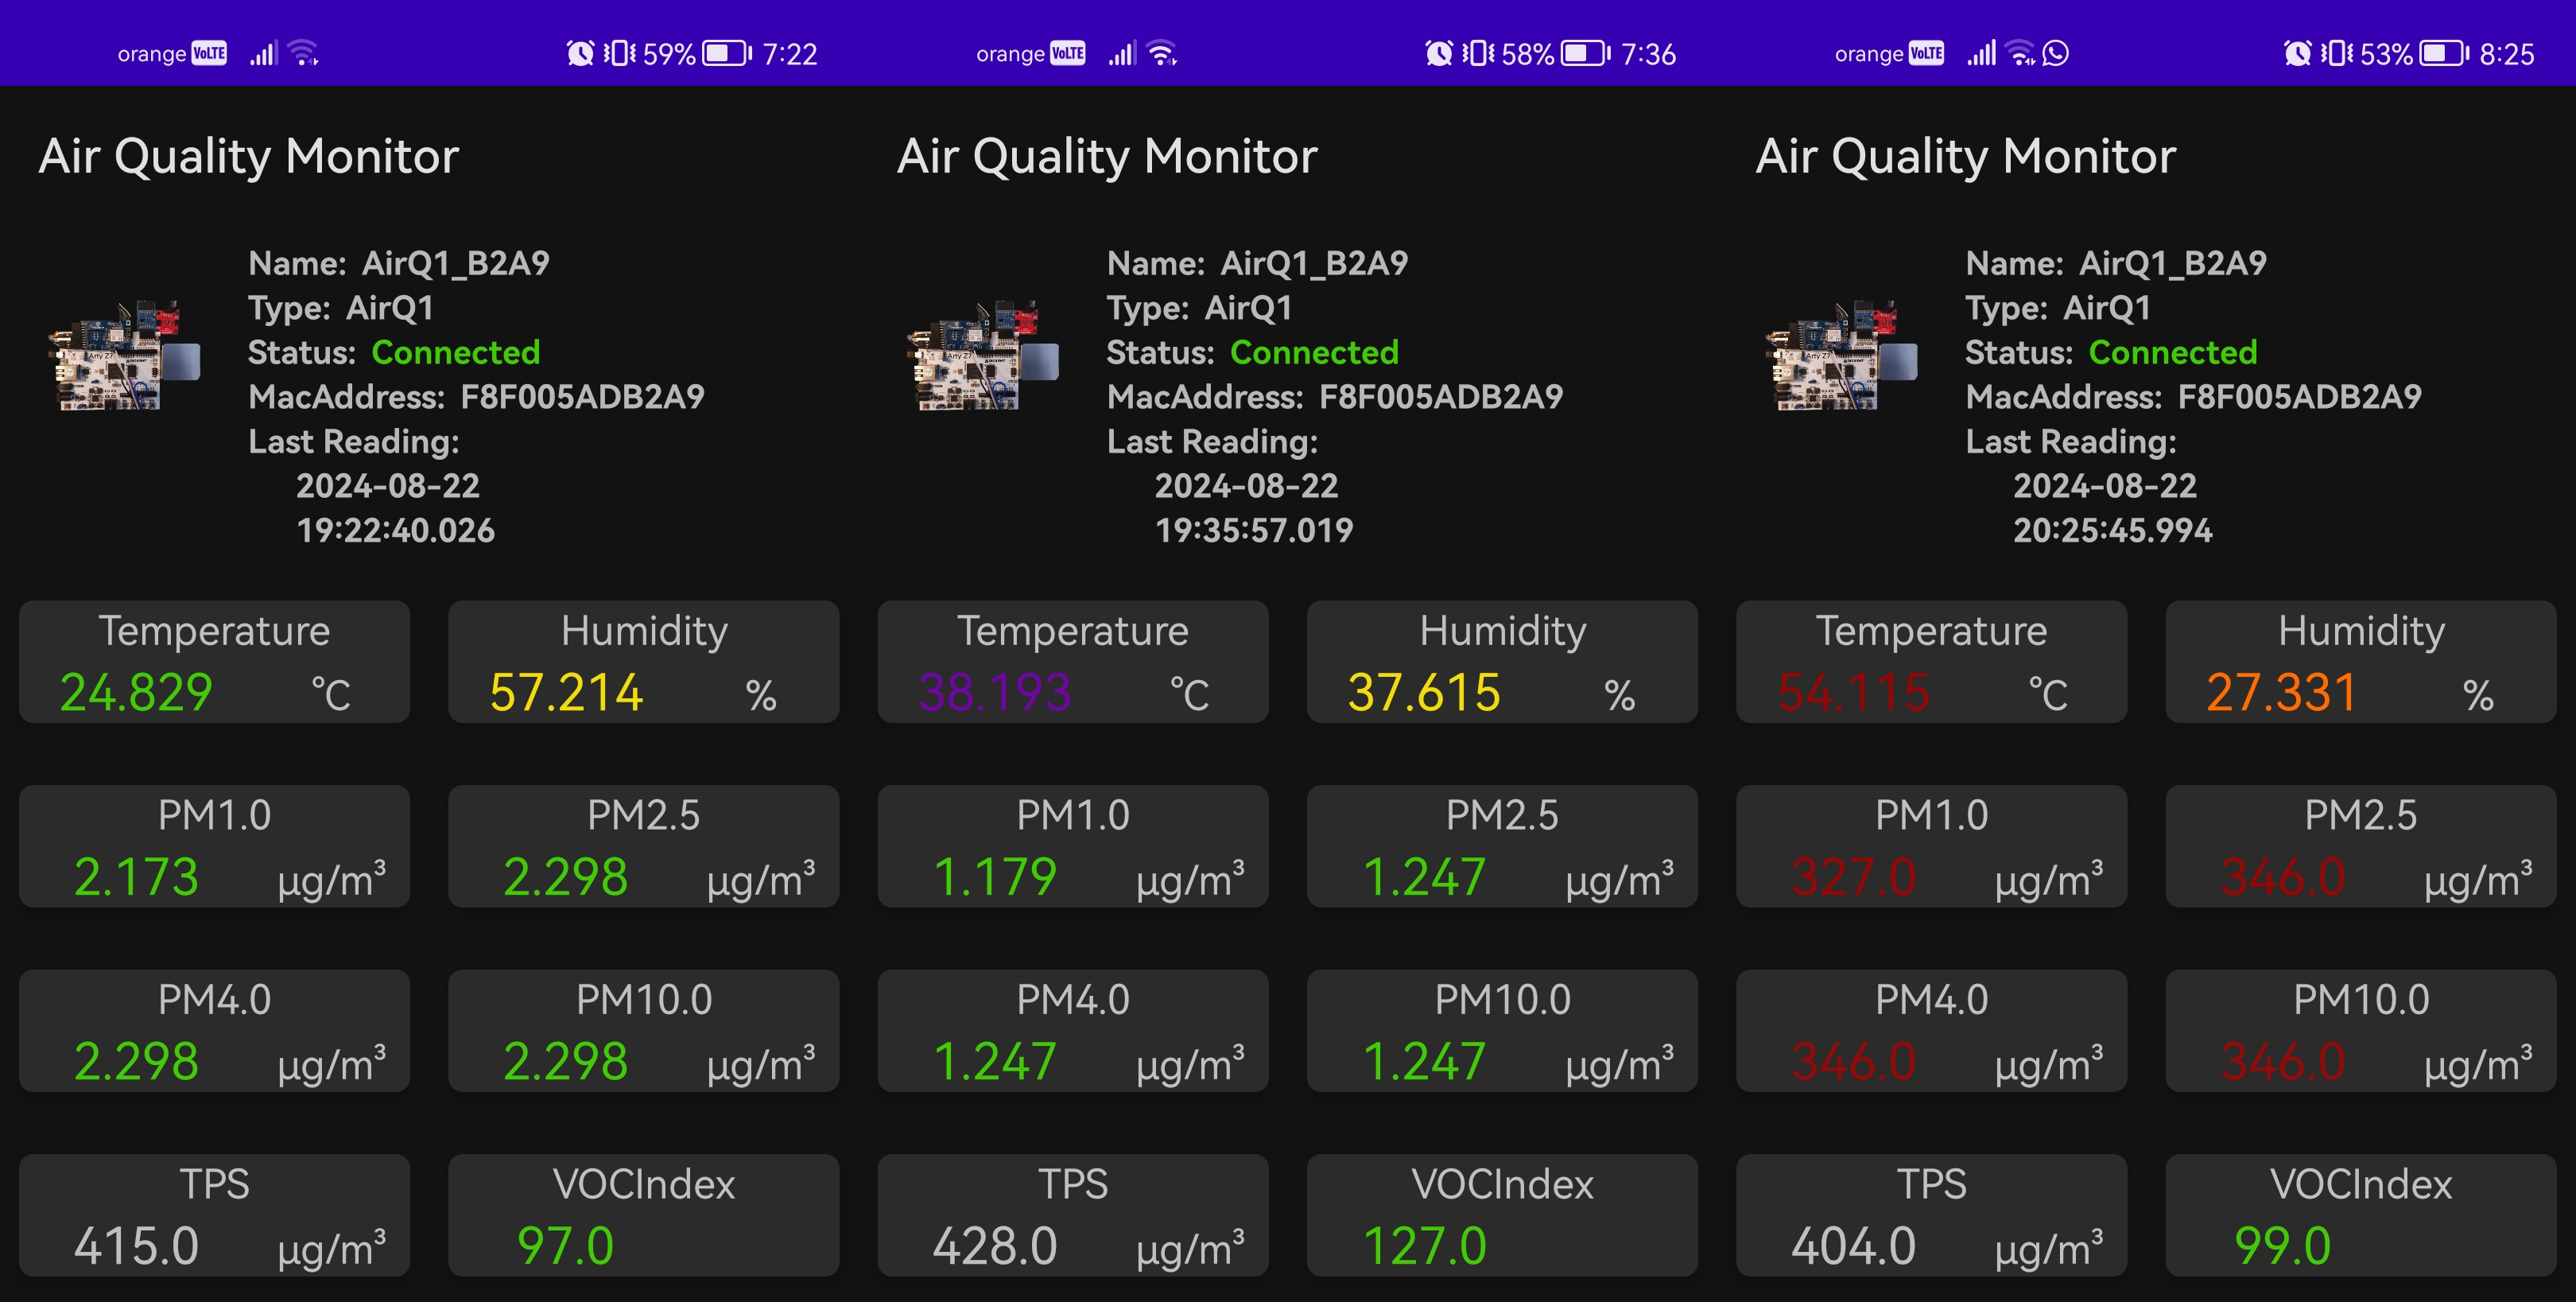
\includegraphics[scale=0.16]{figs/tv_temp_var_sensor_view.png}
    \caption{Valorile indicilor de calitate a aerului in punctele cheie ale testului}
    \label{fig:tv_temp_var_sensor_view}
\end{figure}

Figura \ref{fig:tv_temp_var_chart_view} prezinta 3 capturi de ecran care contin reprezentarea grafica a fiecarui indice de calitate a aerului pe 
intreaga durata a testului.
\begin{figure}[H]
    \centering
    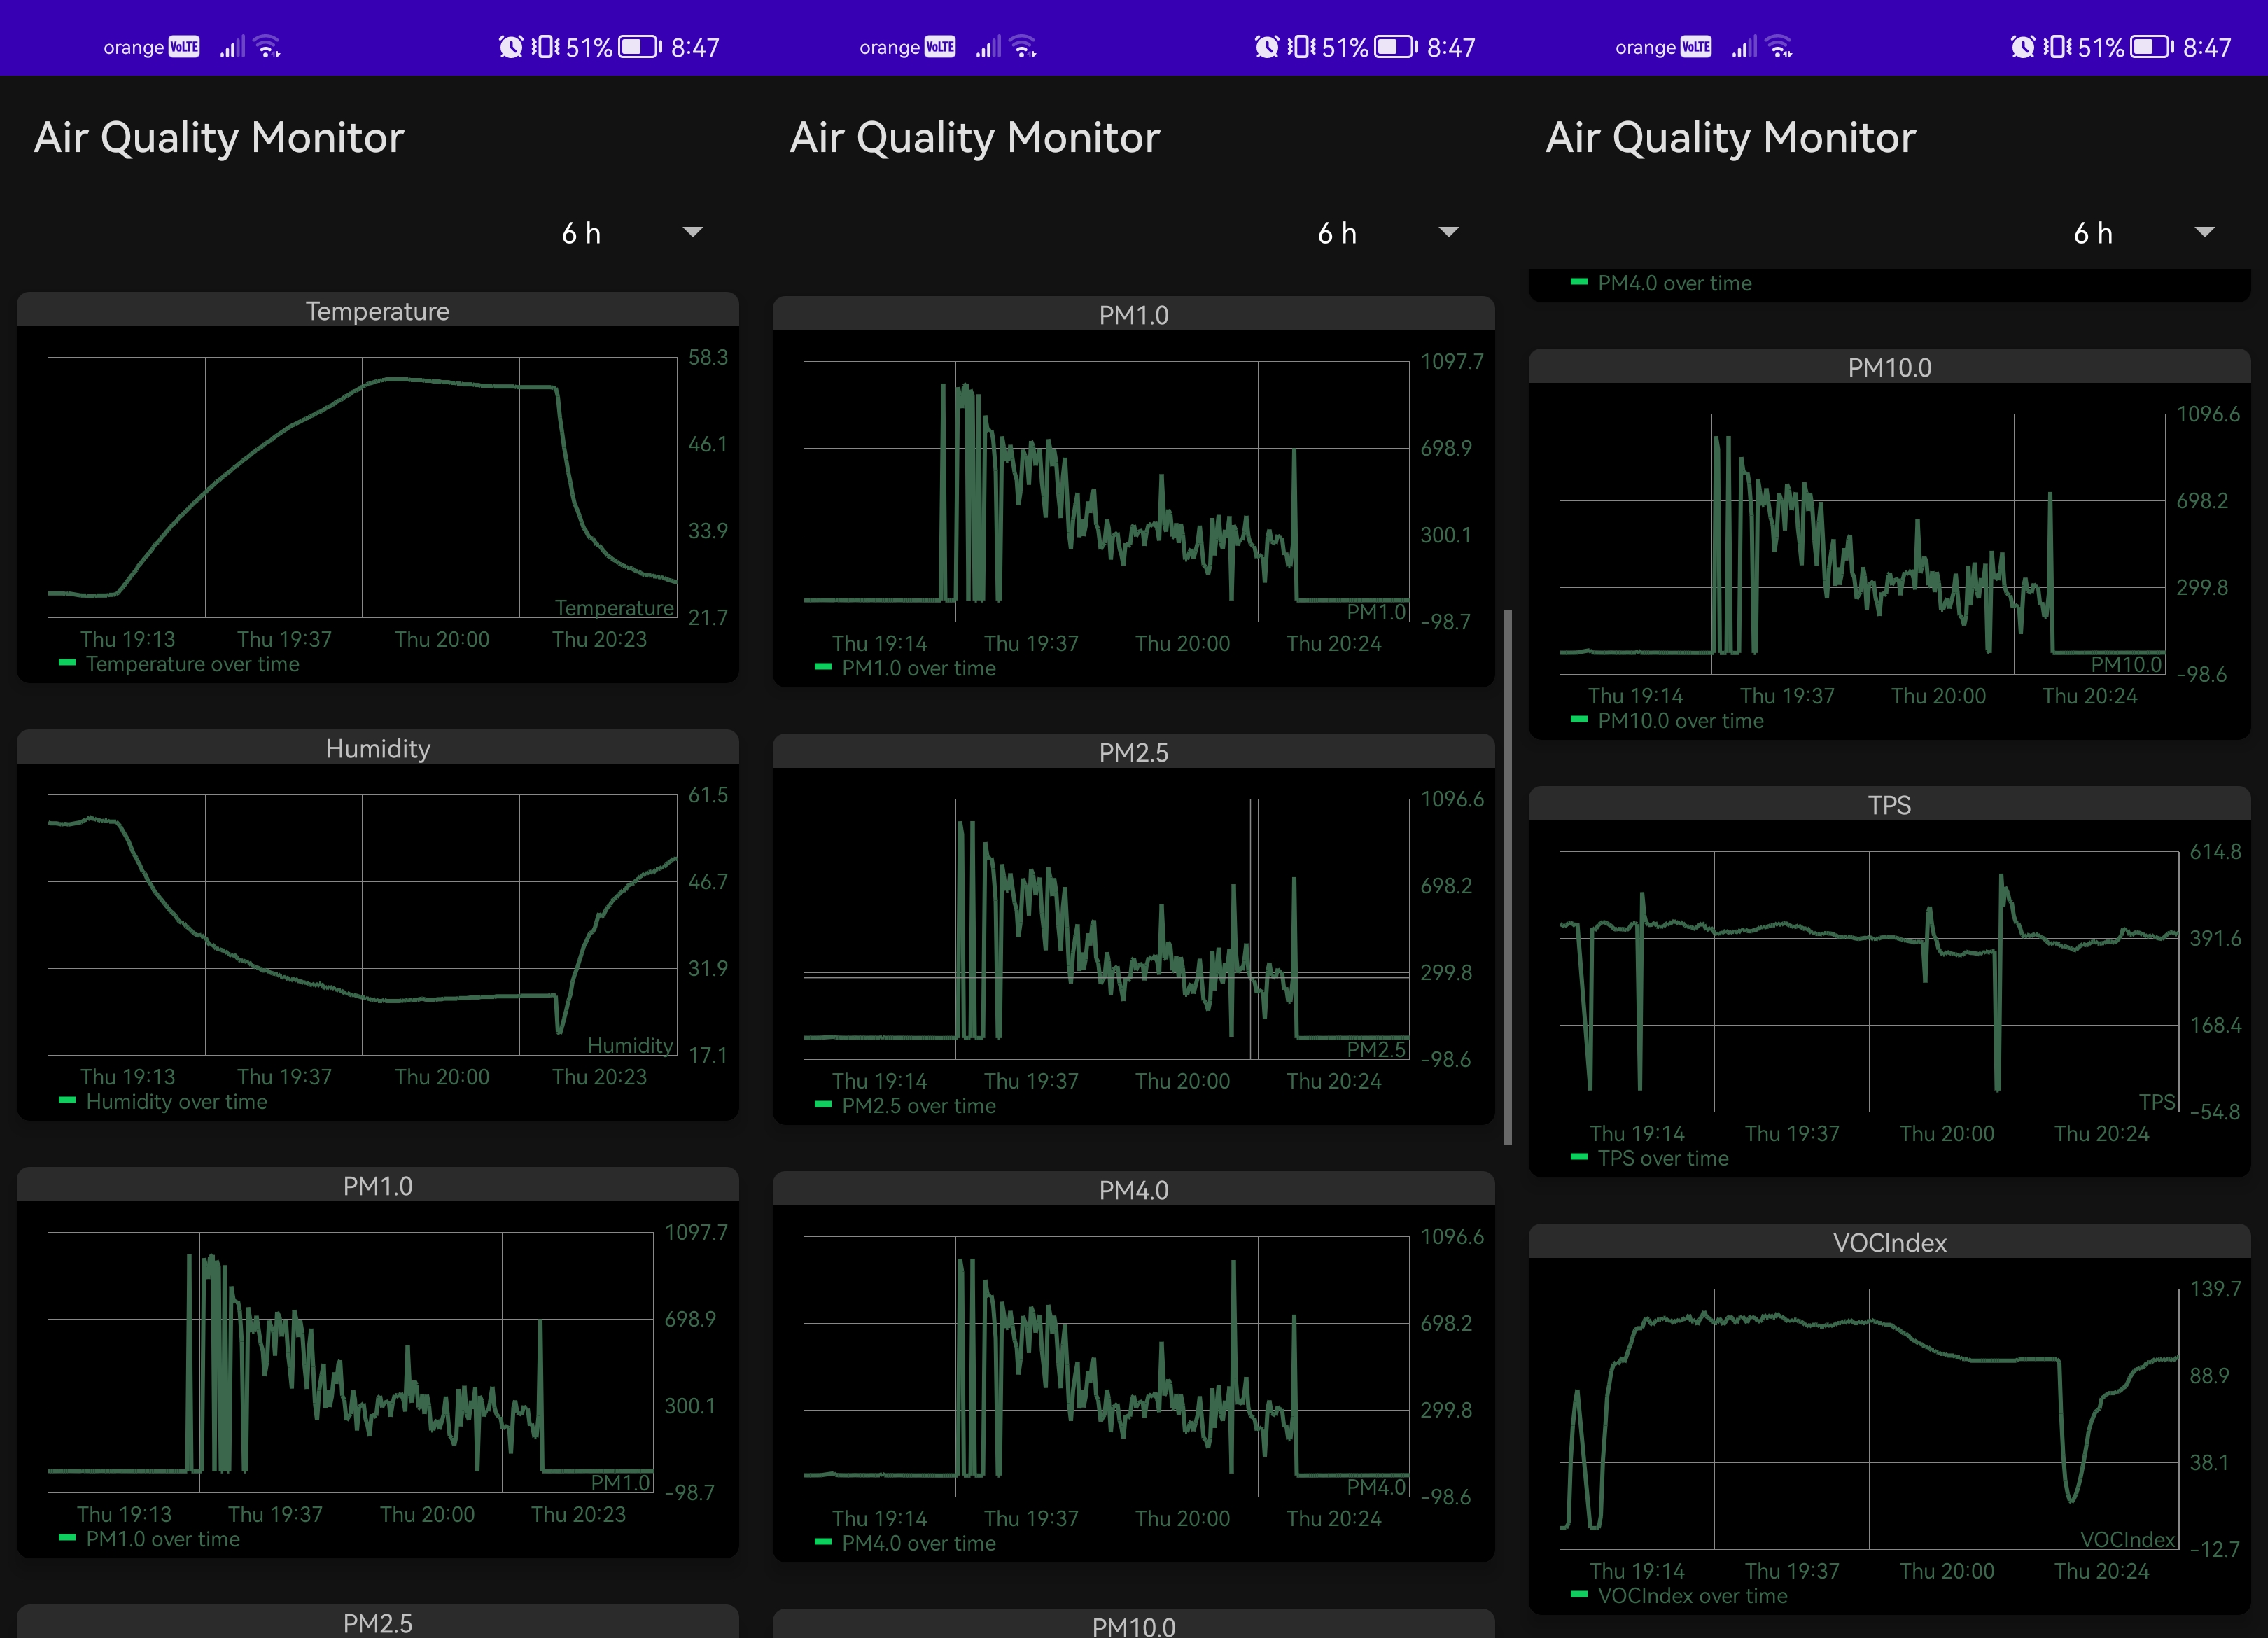
\includegraphics[scale=0.18]{figs/tv_temp_var_chart_view.png}
    \caption{Graficele indicilor de calitate a aerului}
    \label{fig:tv_temp_var_chart_view}
\end{figure}

Figura \ref{fig:tv_temp_var_chart_view} prezinta graficul generat de senzorul camerei termice.
\begin{figure}[H]
    \centering
    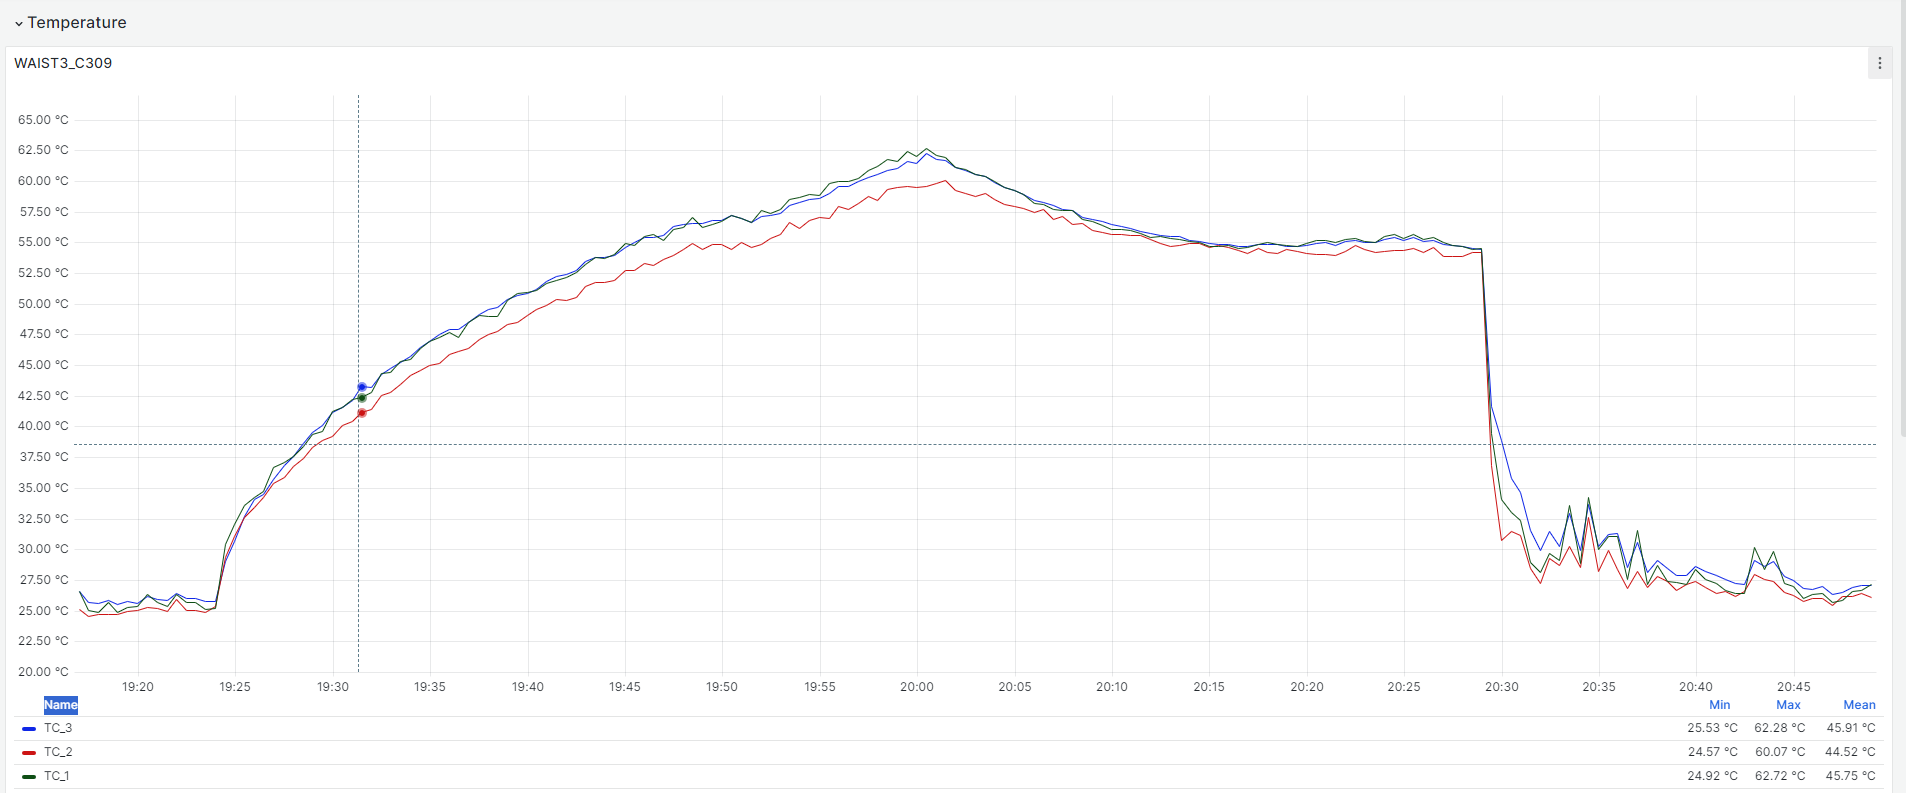
\includegraphics[scale=0.3]{figs/tv_temp_var_waist_chart.png}
    \caption{Graficul senzorului etalon}
    \label{fig:tv_temp_var_waist_chart}
\end{figure}

\subsection{Variatia particulelor in suspensie din aer}
Pentru realizarea acestui test senzorul de calitate a aerului a fost amplasat intr-o cutie de carton pentru a limita dimensiunea mediului la care acesta este expus. 
Printr-o gaura in partea superioara a cutiei a fost introdus in mod treptat fum.

In graficele PM1.0, PM2.5, PM4.0 si PM10.0 din figura \ref{fig:tv_pm_var_chart_view} se observa curbele de crestere si scadere a cantitatii particulelor in suspensie 
pe metru cub. Curba de crestere este destul de brusca, desi s-a incercat introducerea de fum in cantitati foarte mici, ceea ce arata sensibilitatea senzorului SPS30. 
Curba de scadere este foarte abrupta si semnifica momentul deschiderii cutiei si automat aerisirea acesteia. In graficul TPS, care reprezinta cantitatea generala a 
partiulelor in suspensie din aer, a crescut pana la valoarea de 700 micrograme pe metru cub, apoi a intrat in saturatie si a raportat valori sub 2 micrograme pe metru 
cub pana cand cutia a fost deschisa si s-a revenit la valori normale. Graficul de temperatura prezinta o crestere pana la 28.6 grade celsius, iar graficul de umiditate 
prezinta o scadere pe durata testului, ceea ce e normal din moment ce in cutie a fost introdus fum cald.    

Figura \ref{fig:tv_pm_var_chart_view} prezinta 3 capturi de ecran care contin reprezentarea grafica a fiecarui indice de calitate a aerului pe 
intreaga durata a testului.
\begin{figure}[H]
    \centering
    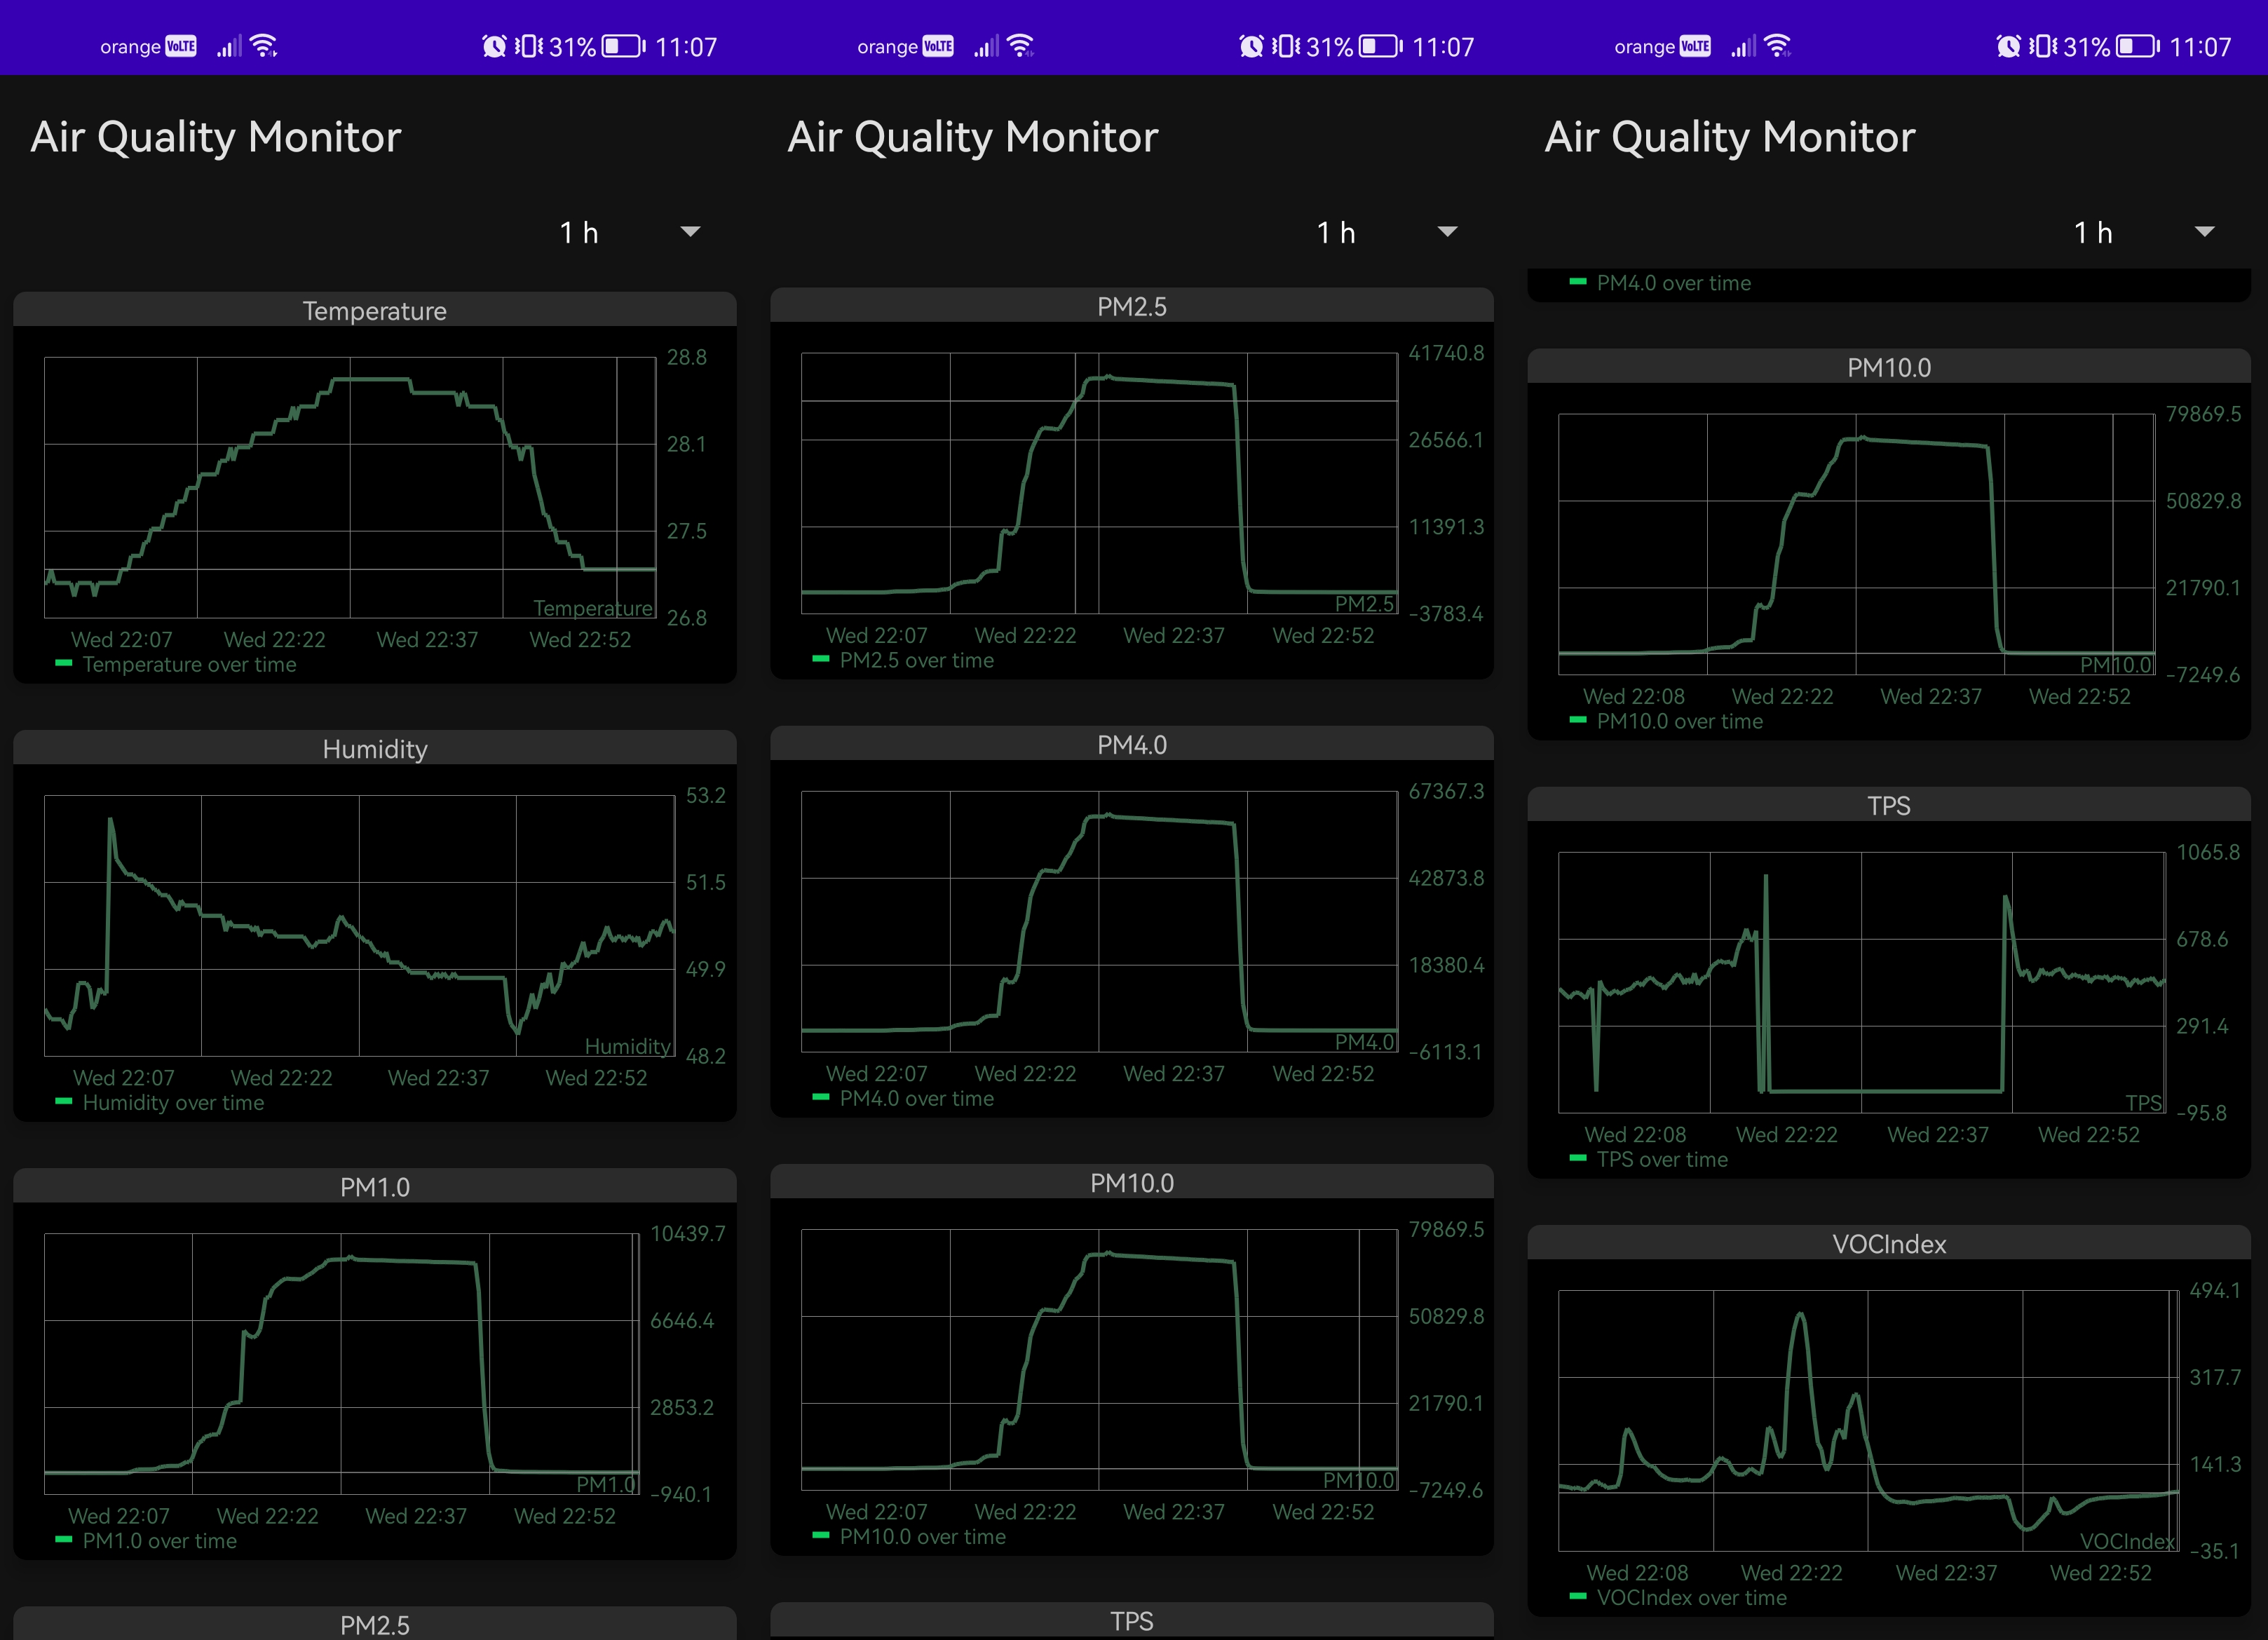
\includegraphics[scale=0.16]{figs/tv_pm_var_chart_view.png}
    \caption{Graficele indicilor de calitate a aerului}
    \label{fig:tv_pm_var_chart_view}
\end{figure}

\section{Test de consum de putere}\label{sec:tv_pwrcons}
Pentru realizarea acestui test s-a utilizat un ampermetru legat in serie cu placa de dezvoltare Arty Z7 si o sursa de curent continuu pentru alimentare. Placa de dezvoltare 
poate fi alimentata la 7-15 V prin conectorul J7 pinii VIN si GND si prin amplasarea unui conector jumper in modul REG de pe setul de pini JP5. Astfel, sursa a fost setata 
pe 12 V, firul rosu de iesire din sursa a fost conectat la intrarea ampermetrului, iesirea ampermetrului conectata la pinul VIN de alimentare a senzorului, iar pinul GND 
al senzorului la firul GND al sursei. Acest test ofera punctul de plecare in imbunatatirea consumului senzorului in viitoare versiuni ale acestuia.

Testul a fost efectuat pe o perioada de 30 de minute in care ampermetrul a esantionat valori ale consumului de putere si a facut o medie a acestora, consumul de putere 
rezultat fiind de 151.11 mA/h.

Figura \ref{fig:tv_pwr_cons} prezinta o captura a ecranului ampermetrului unde sunt afisate sub forma grafica valorile esantionate in ultimele 60 de secunde. Perioada 
de esantionare a fost setata pe 0.02 secunde si limitarea de curent la 1 A. In figura se pot observa cateva varfuri in amplitudinea semnalului, acestea reprezinta 
transmisiile radioului. De asemenea, in figura sunt afisate media (151.11 mA/h), maximul (218.9 mA/h) si minimul (139.0 mA/h) consumului de putere detectate in cele 
30 de minute de functionare.
\begin{figure}[H]
    \centering
    \includegraphics[scale=0.09]{figs/tv_pwr_cons.png}
    \caption{Captura ecran ampermetru digital}
    \label{fig:tv_pwr_cons}
\end{figure}

\section{Scalabilitatea sistemului}\label{sec:tv_scalability}
Acest test are scopul de a demonstra capabilitatea sistemului de monitorizare a calitatii aerului de a gestiona mai multi senzori.

Pentru realizarea testului au fost simulati 20 de senzori utilizand mai multe instante ale unui script scris in limbajul de programare Python. Acest script utilizeaza 
biblioteca Paho MQTT oferita de compania Eclipse sub licenta libera pentru a se conecta la broker-ul MQTT si pentru a publica date cu o periodicitate de 20 de secunde. 
Datele publicate sunt generate prin incrementarea unei variabile inainte de publicarea fiecarui mesaj. Senzorii simulati sunt diferiti de senzorul prezentat in lucrare 
prin faptul ca publica doar date de temperatura si umiditate. S-a ales publicarea acestui set de date pentru a testa capacitatea sistemului de a gestiona un set de date 
diferit si de a valida modificarile care trebuie efectuate cand se doreste utilizarea unui tip de senzor diferit. Pentru crearea mai multor instante a acestui script s-a 
creat un fisier de tip Batch care executa scriptul intr-o bucla care se repeta de 20 de ori. In partea aplicatiei Android, acesti senzori au fost scrisi in memorie ca si 
cum ar fi fost intalati in prealabil. Tipul acestor senzori este "AirQ2", iar tipul senzorului prezentat in lucrare este "AirQ1", acestu lucru se poate observa in prima 
captura de ecran din figura \ref{fig:tv_scalability_welcome_view}. Senzorii simulati au adrese MAC prin care sunt identificati unic incepand de la "000000000001" si pana 
la "000000000020".

In figura \ref{fig:tv_scalability_welcome_view} se poate observa denumirea fiecarui senzor alcatuita din tipul acestuia si ultimele 4 caractere din adresa MAC. Statusul 
conexiunii cu baza de date si cu broker-ul MQTT apare in dreapta fiecarui senzor "Connected". Imaginea senzorilor difera in functie de tipul acestora. 

Testul a fost executat pe o perioada de o ora in care s-a verificat periodic statusul conectivitatii cu baza de date si cu broker-ul MQTT. La finalul testului 
s-a verificat valoarea pe care senzorii o raporteaza. Aceeasi valoare raportata de fiecare senzor inseamna ca nici un pachet nu a fost pierdut. In figura 
\ref{fig:tv_scalability_sensor_chart_view} se poate observa graficul generat pe intreaga perioada de testare.

Figura \ref{fig:tv_scalability_welcome_view} prezinta 3 capturi de ecran reprezentand inceputul, mijlocul si finalul listei senzorilor.
\begin{figure}[H]
    \centering
    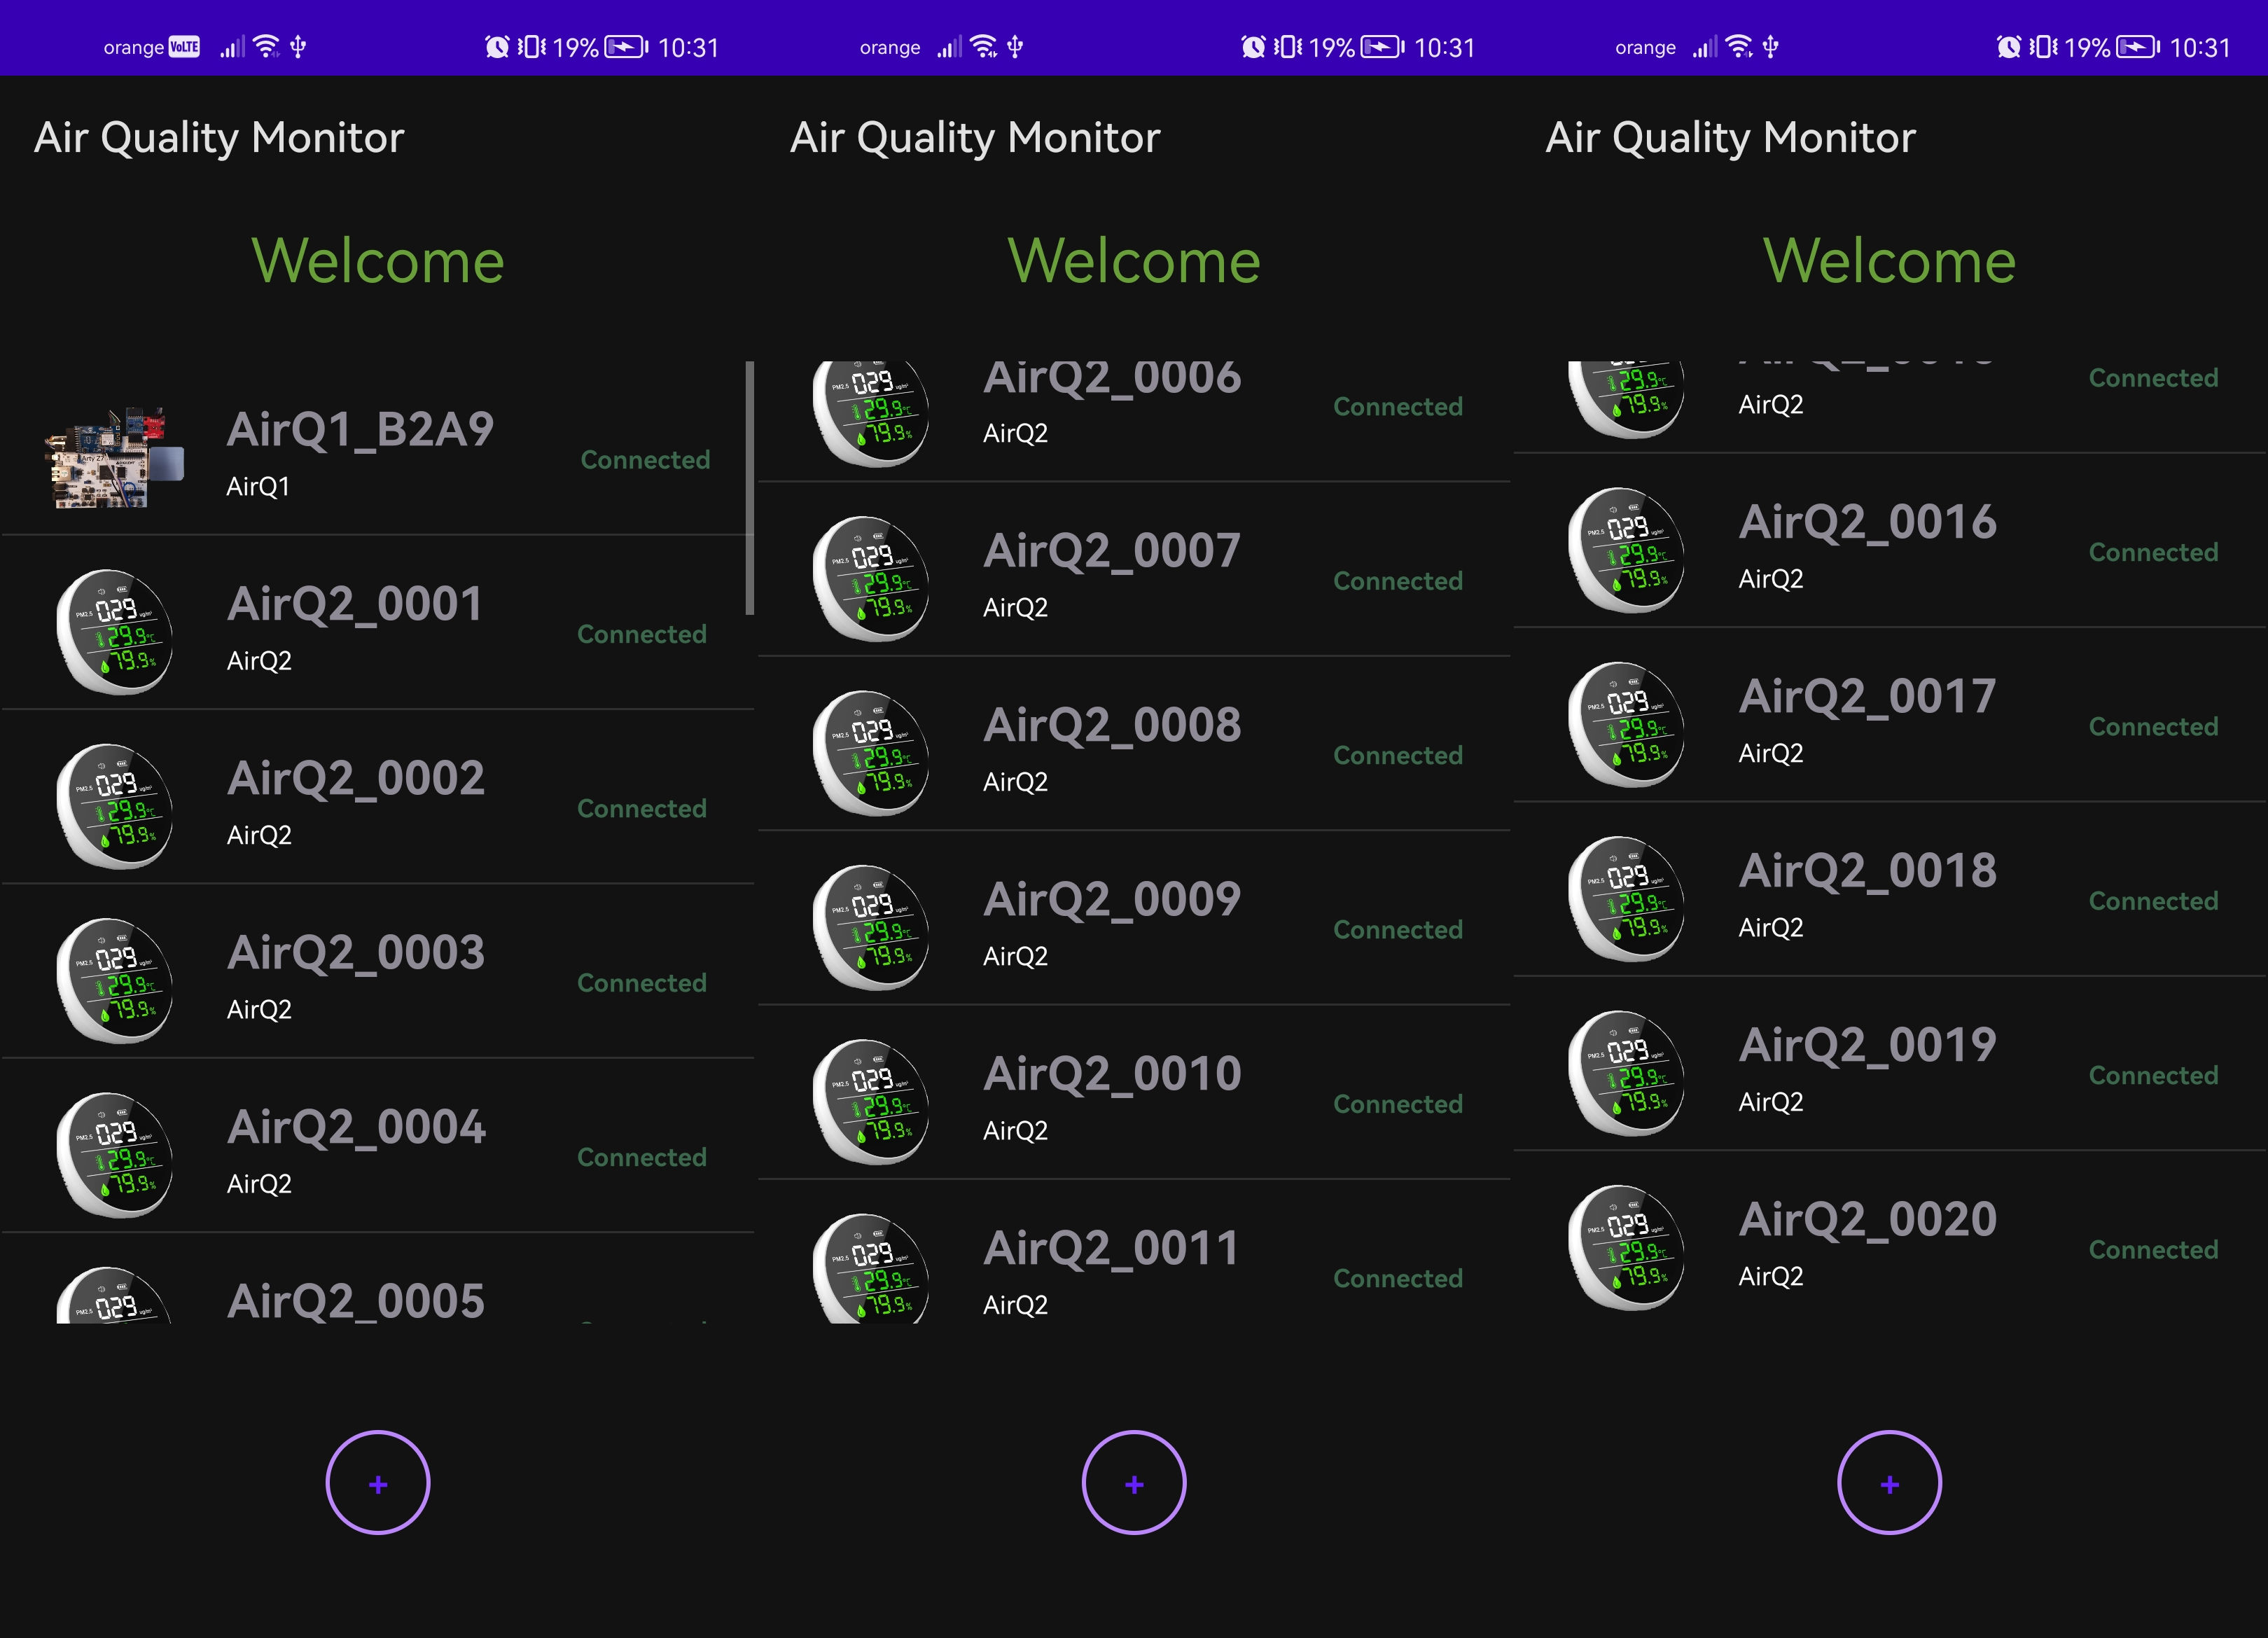
\includegraphics[scale=0.16]{figs/tv_scalability_welcome_view.png}
    \caption{Lista senzorilor din aplicatia Android}
    \label{fig:tv_scalability_welcome_view}
\end{figure}

Figura \ref{fig:tv_scalability_sensor_chart_view} prezinta 2 capturi de ecran reprezentand informatiile unuia dintre senzorii simulati, ultimele valori de temperatura 
si umiditate raportate de acestia si graficele pe intreaga durata a testului.
\begin{figure}[H]
    \centering
    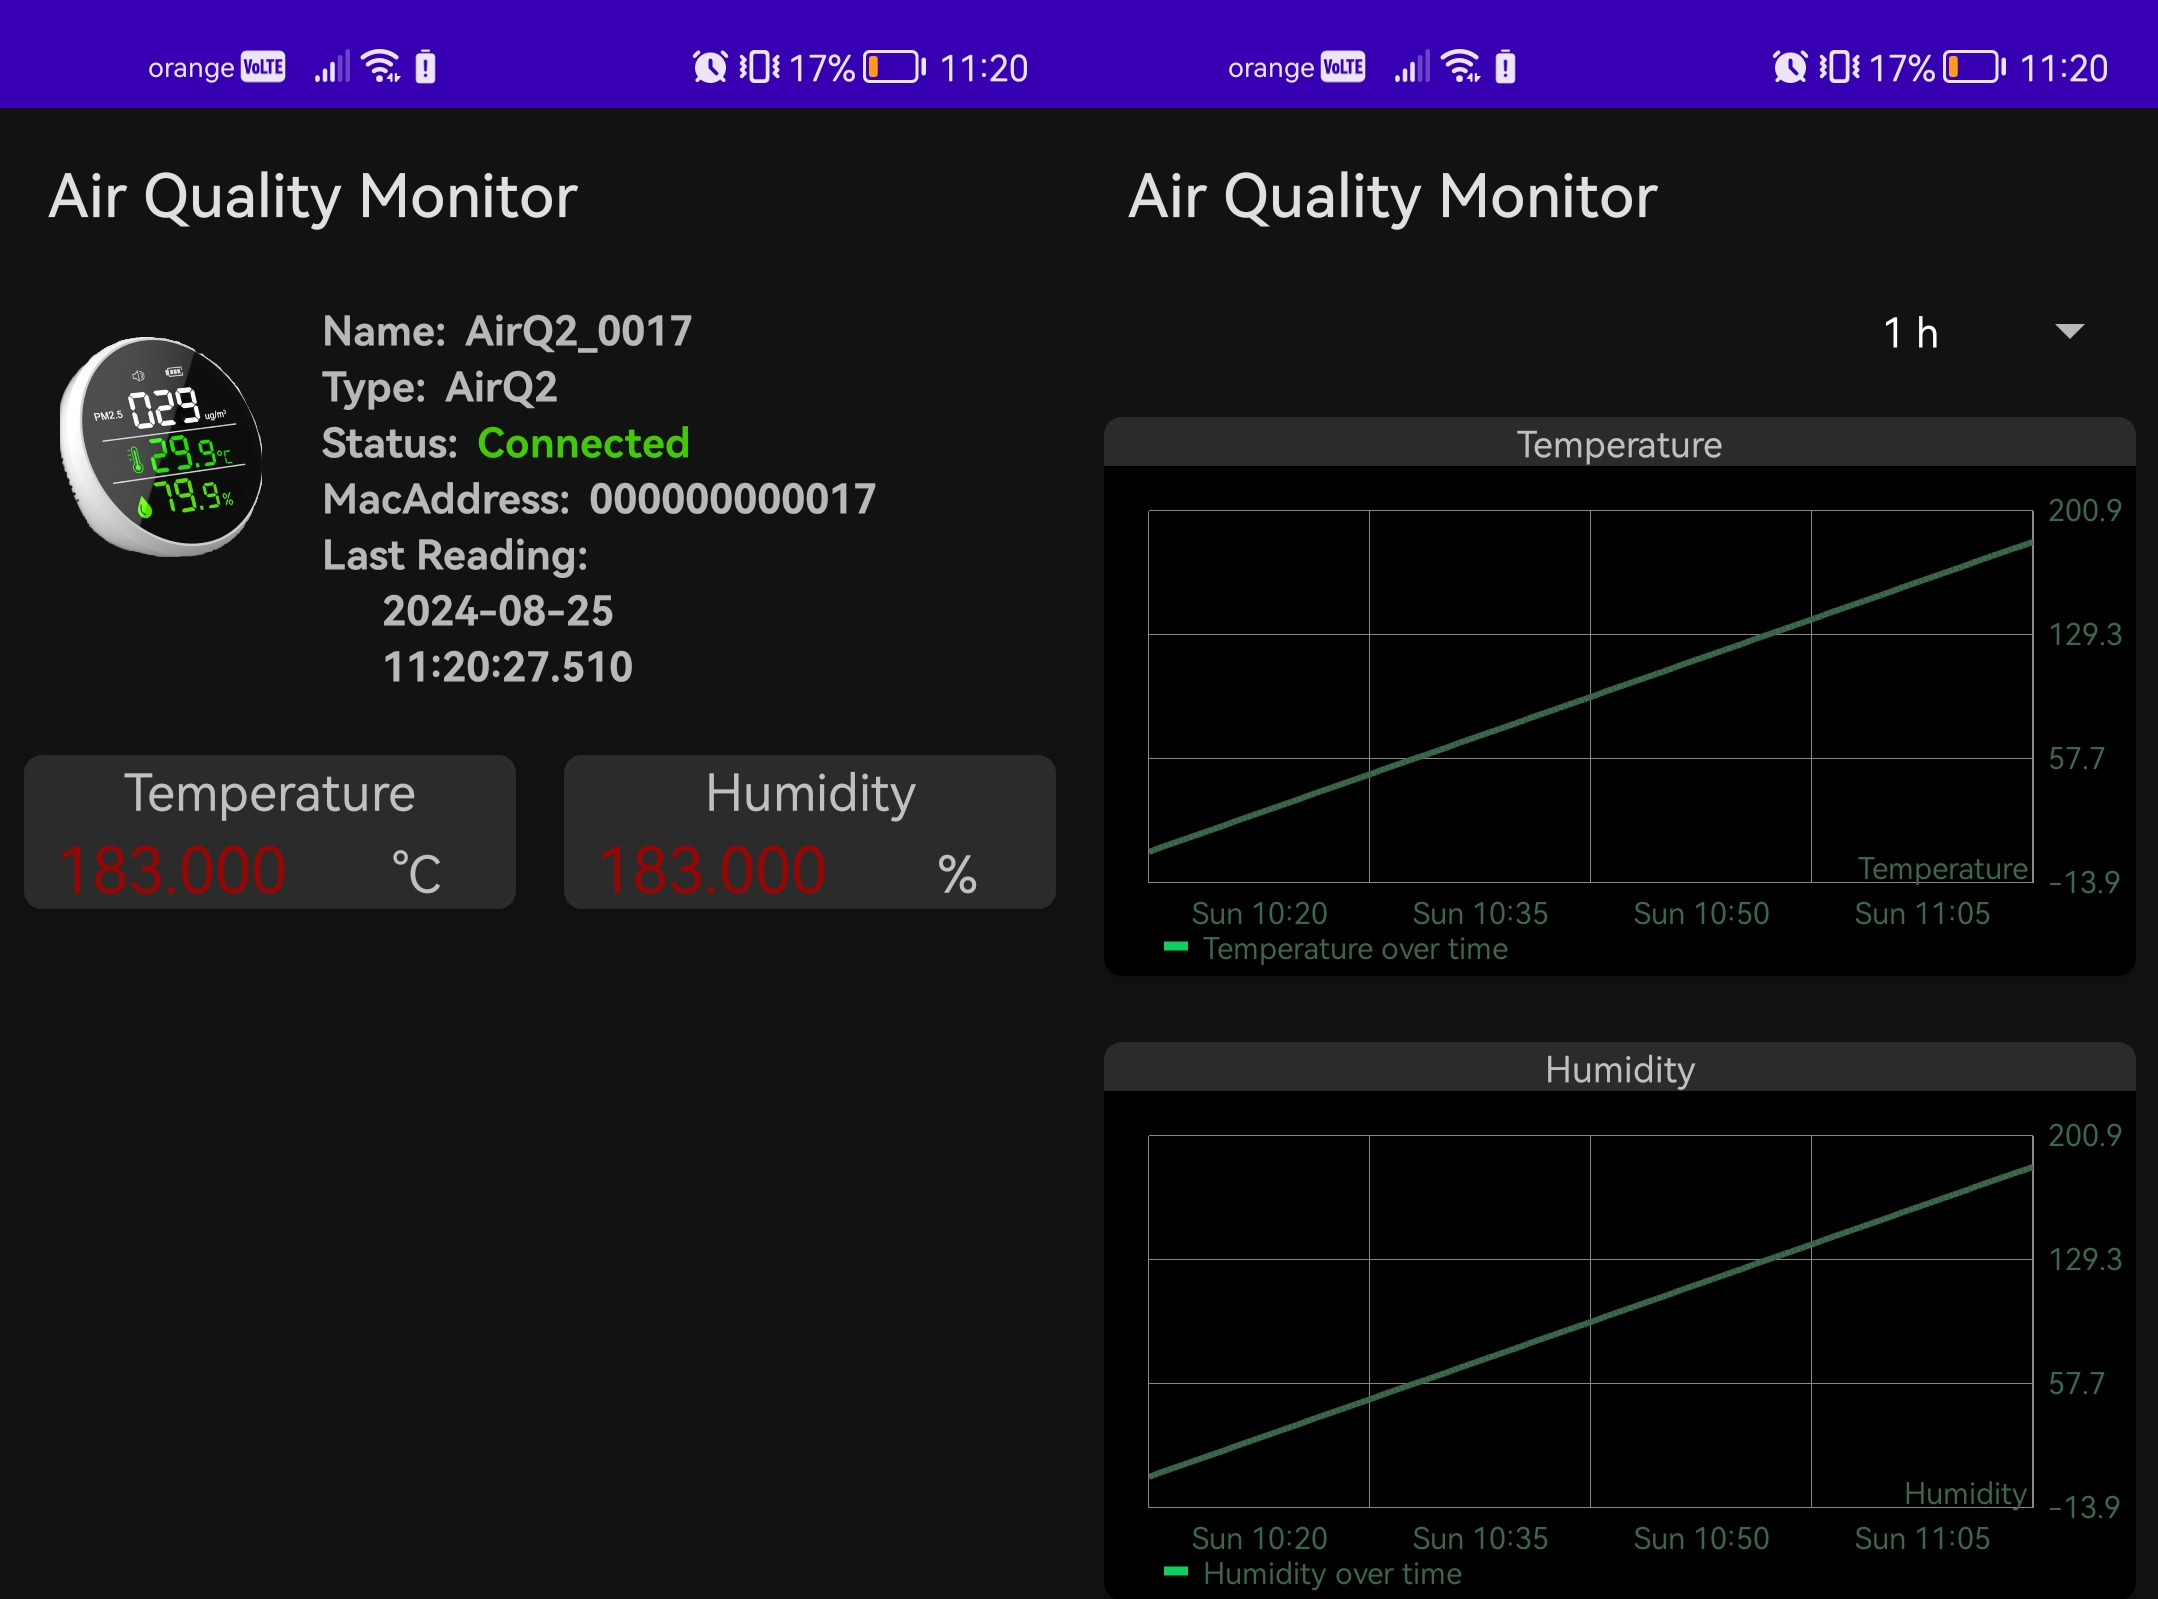
\includegraphics[scale=0.18]{figs/tv_scalability_sensor_chart_view.png}
    \caption{Valorile si graficele de temperatura si umiditate la finalul testului}
    \label{fig:tv_scalability_sensor_chart_view}
\end{figure}

\section{Latenta sistemului}\label{sec:tv_latecy}
Acest test are scopul de a calcula cat dureaza ca datele sa ajunga in diferite module ale sistemului de monitorizare a calitatii aerului. Pentru realizarea testului au 
fost adaugate in codul sursa linii de cod care afiseaza timpul curent. In cazul senzorului s-a utilizat un terminal serial care afiseaza momentul de timp cand un mesaj a 
fost receptionat.

Latenta sistemului este impartita in 3 categorii, latenta in cazul datelor in timp real notata T\_real, latenta in cazul datelor istorice notata T\_istoric si 
latenta in cazul salvarii in baza de date notata T\_db.

T\_real este impartita in mai multe puncte si reprezinta durata de timp din momentul inceperii esantionarii datelor si pana la afisareaa acestora pe ecran:
\begin{itemize}
	\item T\_senzor - durata timpului din momentul inceperii achizitiei si pana la transmisia datelor catre aplicatie.
	\item T\_senzor\_app - durata timpului din momentul in care datele au fost transmise catre aplicatie si pana in momentul in care ele au ajuns in aplicatie.
	\item T\_app\_screen - durata timpului din momentul in care datele au intrat in aplicatia Android si pana la aparitia acestora pe ecran.
\end{itemize}

Ecuatia finala este: T\_real = T\_senzor + T\_senzor\_app + T\_app\_screen care este egala cu T\_real = 279ms + 1276ms + 69ms rezultand T\_real = 1.624 secunde 
din momentul inceperii achizitiei si pana la afisareaa datelor pe ecran.

T\_istoric reprezinta durata de timp din momentul in care s-a inceput interogarea bazei de date si pana in momentul in care datele sunt afisate in grafic. Acesta 
poate fi de mai multe feluri in functie de perioada pe care se face interogarea:
\begin{itemize}
	\item T\_istoric\_10m - cazul in care sunt interogate datele din ultimele 10 minute (134 milisecunde).
	\item T\_istoric\_30m - cazul in care sunt interogate datele din ultimele 30 de minute (150 milisecunde).
	\item T\_istoric\_1h - cazul in care sunt interogate datele din ultima ora (176 milisecunde).
	\item T\_istoric\_6h - cazul in care sunt interogate datele din ultimele 6 ore (634 milisecunde).
	\item T\_istoric\_1d - cazul in care sunt interogate datele din ultimele 24 de ore (1.556 secunde).
\end{itemize}

T\_db reprezinta durata de timp din momentul inceperii esantionarii de date si pana in momentul in care datele sunt salvate in baza de date. Acesta este impartit 
in mai multe puncte:
\begin{itemize}
    \item T\_senzor - durata timpului din momentul inceperii achizitiei si pana la transmisia datelor catre aplicatie.
	\item T\_api - durata timpului din momentul in care senzorul a trimis datele si pana in momentul in care datele au fost receptionate de interfata bazei de date.
	\item T\_saved - durata timpului din momentul in care interfata bazei de date a primit cererea HTTP si pana in momentul in care datele au fost salvate in baza 
    de date.
\end{itemize}

Ecuatia finala este: T\_db = T\_senzor + T\_api + T\_saved care este egala cu T\_db = 279ms + 1097ms + 3ms rezultand T\_db = 1.379 secunde 
din momentul inceperii achizitiei si pana la afisareaa datelor pe ecran.

Pe intreaga perioada de testare au fost functionali cei 20 de senzori simulati pentru testul din capitolul \ref{sec:tv_scalability}, deci intervalele de timp 
prezentate in acest capitol au fost esantionate pe o retea de 21 de senzori. % \chapter{Testare și Validare}

\chapter{Manual de instalare și utilizare}
\pagestyle{fancy}

În secțiunea de Instalare trebuie să detaliați resursele software și hardware necesare pentru instalarea și rularea aplicației, precum și o descriere pas cu pas a procesului de instalare.

Instalarea aplicației trebuie să fie posibilă pe baza a ceea ce se scrie aici.

În acest capitol trebuie să descrieți cum se utilizează aplicația din punct de vedere al utilizatorului, fără a menționa aspecte tehnice interne.

Folosiți capturi ale ecranului și explicații pas cu pas ale interacțiunii.

Folosind acest manual, o persoană ar trebui să poată utiliza produsul vostru.

{\noindent\color{blue} Între 1 și 5 pagini.\\} % \chapter{Manual de Instalare și Utilizare}

\chapter{Concluzii}
\pagestyle{fancy}

Acest capitol va fi prezentat in 3 sectiuni, contributiile personale aduse domeniului monitorizarii calitatii aerului, analiza rezultatelor obtinute in urma 
dezvoltarii lucrarii de fata si posibile dezvoltari ulterioare.

\section{Contributii personale}\label{c_contributii}
Integrarea protocolului MQTT cu procesorul Zynq 7000 si imbunatatirea performantei driver-ului Paho MQTT oferit de Eclipse care este executat pe senzor prin 
inlocuirea portiunilor de cod unde se utiliza blocarea buclei sistemului in asteptarea unui eveniment cu o semaforizare bazata pe module Timer.

Integrarea controller-ului de retea ATWINC1500 cu procesorul Zynq 7000 ofera posibilitatea de a concentra puterea de procesare a cipului pe achizitia datelor de 
la senzorii de calitate a aerului si, intr-o dezvoltare ulterioara, de a executa algoritmi constisitori pentru procesarea acestor date, gestiunea 
retelei fiind integrata in controlerul de retea.

Structurarea datelor raportate de senzori conform cu cerintele bazei de date de tip serii in timp pentru a beneficia de toate avantajele acesteia, performante 
foarte bune la scriere si interogare, capacitate de stocare mare si un grad inalt de scalabilitate.

Raportarea parametrilor de calitate a aerului PM4.0 (particule in suspensie cu diametru mai mic de 4 micrometri) si TPS (media diametrului particulelor detectate) 
care nu se regasesc in standardele existente de calitate a aerului sau in sistemele de calitate a aerului uzuale, dar care ofera informatii utile despre sursa si 
tipul particulelor detectate.

\section{Analiza rezultatelor}\label{c_analiza_rezultate}
In urma testelor efectuate pe sistem s-a constatat ca vizualizarea si interactiunea cu graficele pe un ecran atat de mic cum este cel al unui telefon este dificila. La 
afisarea datelor istorice pe o perioada mai lunga, cum ar fi o saptamana sau mai mult, se pierd multe informatii din cauza afisarii acestora intr-un grafic restrans 
ca dimensiune. 

Utilizarea sistemului pe o perioada indelungata din punctul de vedere al unui utilizator care a achizitionat acest sistem a demonstrat utilitatea acestuia si necesitatea 
de a fi integrat in spatiile inchise. Observarea in a aplicatie a unor valori care prezinta o calitate a aerului slaba a generat cautarea si inlaturarea sursei problemei. 
De exemplu, necesitatea aerisirii incaperii dupa cateva ore de gatit, deoarece indexul compusilor oranici volatili a depasit pragul unei bune calitati a aerului.

\section{Dezvoltari ulterioare}\label{c_dezvoltari_ulterioare}
Imbunatatirea consumului de putere pentru adaptarea sistemului la functionarea pe baterii. In sectiunea \ref{sec:tv_pwrcons} a fost prezentat consumul senzorului de 
calitate a aerului de 150 mA/h. Scaderea acestui consum implica limitarea utilizarii led-urilor strict la procesul de instalare, activarea perifericelor de comunicatie 
I2C si SPI doar atunci cand sunt utilizate pentru o achizitie de date, implementarea modului de consum de putere redus (Low Power Mode) pe Zynq 7000, activarea modului 
de consum redus pe senzori si pe controllerul de retea atunci cand nu sunt utilizati, etc. Consumul de putere ar trebui sa ajunga la o valoare care sa permita utilizarea 
senzorului in mod continuu timp de minim un an.

Integrarea senzorului intr-un sistem comun de monitorizare a calitatii aerului. Asa cum a fost prezentat in capitolul \ref{ch:studiubib} exista mai multe sisteme care pun 
la dispozitia populatiei harta lumii impanzita de senzori de calitate a aerului a caror date pot fi vizualizate in timp real.

 % \chapter{Concluzii}

\bibliographystyle{IEEEtran}
\bibliography{licenta}%same file name as for .bib

\appendix
\chapter{Secțiuni relevante din cod}
\pagestyle{fancy}

\begin{verbatim}
 /** Maps are easy to use in Scala. */
object Maps {
  val colors = Map("red" -> 0xFF0000,
                   "turquoise" -> 0x00FFFF,
                   "black" -> 0x000000,
                   "orange" -> 0xFF8040,
                   "brown" -> 0x804000)
  def main(args: Array[String]) {
    for (name <- args) println(
      colors.get(name) match {
        case Some(code) =>
          name + " has code: " + code
        case None =>
          "Unknown color: " + name
      }
    )
  }
}
\end{verbatim}

\chapter{Alte informații relevante (demonstrații etc.)}

{\color{blue}Se va elimina dacă nu există}

\chapter{Lucrări publicate (dacă există)}

{\color{blue}Se va elimina dacă nu există}

\end{document}
